%   thesis.tex - UAH Master's Thesis Main TeX file
%
%   This is the main file for my thesis. It loads all content via
%   \include statments

%%% Making the DVI and PDF output the correct size %%%
%   Important - the default pagesize for DVI and PDF output in most LaTeX
%   distributions is a4 (210x297cm, or about 8.27�11.69 in), which won't work
%   for the UAH format.  So, you have to change the DVI and PDF output in your
%   LaTeX distribution.  In most distros, you need to change the following files:

%   (1.)  C:\texmf\dvipdfm\config\dvipdfmx.cfg
%   (2.)  C:\texmf\dvipdfm\config\config
%   (3.)  C:\texmf\pdftex\config\pdftex.cfg

%   For numbers (1.) and (2.), you will change where the files say "p a4" to
%   "p letter" (there should be some explanation in the files themselves, too).
%   For number (3.), you will change two lines of that file to read:

%   page_height 11 true in
%   page_width 8.5 true in

%   There are "local" versions of all the above files in this complete rar
%   package which 'should' override the a4 defaults - but these do not work in
%   some distributions, so editing the above files is usually necessary.
%   For more info, search google for "pdftex.cfg" and "dvipdfmx.cfg"
%%% (End DVI and PDF changes) %%%

%   Define the document class. The proper class is "book." The normal options
%   are "12pt" and "onesided". When printing out copies for purposes other than
%   submission to the Graduate School, the option "twoside" can be used to
%   format the output in a manner which looks good when printed duplex.

\documentclass[12pt,oneside,letterpaper]{book}

%   Load the packages necessary for the thesis. The only required packages are
%   "uahdis", which loads the UAH Dissertation Style, and "chngpage" which is
%   used by "uahdis". The other packages are optional, and should be loaded only
%   if you have a need for the functionality they provide. Documentation on each is
%   available at CTAN.org. The basic purpose of each are described below:
%   units---provides a convenient mechanism for writing quantities with units.
%   bm---provides a convenient mechanism for producing bold symbols in math mode
%   hhline---improved lines and borders in tables
%   rotating---allows landscape oriented pages in a portrait oriented document
%   verbatim---prints text files verbatim. useful for computer code
%   amsfonts---provides additional typefaces
%   amssymb---provides additional mathematical symbols
%   xspace---properly adjusts space after \newcommands which expand to text
%   booktabs---creates traditional scientific tables - no vertical lines, very
%   few horizontal lines, with varying thickness (not meant to be used with hline)

%   Excellent descriptions of all LaTeX packages can be found here:
%   http://www.tug.org/tex-archive/help/Catalogue/index.html

\usepackage[]{uahdis,chngpage,units,bm,hhline,rotating,verbatim,amsfonts,amssymb,xspace}
\usepackage[]{indentfirst,layouts, booktabs, enumerate, gensymb}
\usepackage[]{typedref}
\usepackage[final]{graphicx}
\usepackage{tikz}
\usepackage{mathtools}
\usepackage{mathrsfs}
\usepackage{pdfpages}
\usetikzlibrary{shapes,arrows}
\usetikzlibrary{automata,positioning}
%\usepackage[section]{placeins}
%   Load the tex file which contains all local \newcommands and \newenvironments

%%%
%%% Environments
%%%

\newsavebox{\speaker}
\newenvironment{chapterquote}[1]
    {\begin{flushright}\begin{minipage}{3 in}\sbox{\speaker}{#1}\itshape\singlespace}
    {\begin{flushright}---\usebox{\speaker}\end{flushright}\end{minipage}\end{flushright}}

% Note: chapterquote works (and looks) best when the chapter begins with a \section{} ...
% If you hadn't planned on beginning the chapter with a \section, try \section{Overview} :-)
% otherwise, some \vspace{} might be necessary, but that won't be consistent throughout the thesis

%%%
%%%  Functions---Commands that take parameters
%%%
\newcommand{\cfig}[3]{\centering\includegraphics[keepaspectratio=true,width=#3in]{./CH#1/EPSFDocs/#2}}
\newcommand{\acro}[1]{\textsc{#1}}
\newcommand{\sci}[2]{\ensuremath{#1 \!  \times \!  10^{#2}}}
\newcommand{\vect}[1]{\boldsymbol{\mathbf{#1}}}
\newcommand{\unitvec}[1]{\vect{\hat{#1}}}
\newcommand{\threebythree}[9]{\renewcommand{\arraystretch}{0.75}\begin{vmatrix}#1&#2&#3\\#4&#5&#6\\#7&#8&#9\end{vmatrix}\renewcommand{\arraystretch}{1.0}}
\newcommand{\mysci}[2]{\ensuremath{#1 \!  \times \!  10^{#2}}}
\newcommand{\myprop}[5]{g(#1,#2;#3,#4;#5)}
\newcommand{\myint}[3]{\int_{#1}^{#2}#3}
\newcommand{\myintinfinf}[1]{\myint{-\infty}{\infty}{#1}}


%%%
%%%  New Math Operators
%%%

\DeclareMathOperator{\polylog}{Li}


%%%
%%%  Symbols---Commands that are shorthand
%%%
\newcommand{\rf}{\acro{rf}\xspace}
\newcommand{\dc}{\acro{dc}\xspace}
\newcommand{\ac}{\acro{ac}\xspace}
\newcommand{\ccd}{\acro{ccd}\xspace}
\newcommand{\mach}{\acro{mach2}\xspace}
\newcommand{\mgmhd}{\acro{mgmhd}\xspace}
\newcommand{\cea}{\acro{cea}\xspace}
\newcommand{\half}{\nicefrac{1}{2}\,}
\newcommand{\xx}{\ensuremath{\unitvec{x}}\xspace}
\newcommand{\yy}{\ensuremath{\unitvec{y}}\xspace}
\newcommand{\zz}{\ensuremath{\unitvec{z}}\xspace}
\newcommand{\ttl}{\acro{ttl}\xspace}
\newcommand{\pmt}{\acro{pmt}\xspace}
\newcommand{\eg}{\textit{e.g.}\xspace}
\newcommand{\ie}{\textit{i.e.}\xspace}
\newcommand{\qmn}{\ensuremath{q^{mn}}\xspace}
\newcommand{\isp}{\ensuremath{I_{sp}}\xspace}



%%%
%%%  Other stuff I've found - Evaluate for usefulness
%%%

%\newcommand{\quan}[2][]{\mbox{$#1\,\mathrm{#2}$}}
%\newcommand{\vv}[1]{\ensuremath{\boldsymbol{#1}}}
%\newcommand{\tempc}[1]{\quan[#1]{^{\circ}C}}
%\DeclareMathOperator{\sinc}{sinc}
%\newcommand{\comment}[1]{\marginpar{\Large \hfill \ddag}\textsf{#1}}
%\newcommand{\comment}[1]{}


%   The next line requires the leading "%". It is only useful if you are using
%   WinEdt as your text editor. It allows WinEdt to collect bibliographic entries into
%   a pop-up table that you can summon when you are \cite-ing a source.

%GATHER{Bibliography.bib}

%   Define my name
\author{Joshua A. Fowler}

%   Define the title of my thesis (user upper and lower case)
\title{High Order Roe-WENO Schemes Based on Higher-Order Central Differencing and Reconstruction}

%   Define the year
\date{2021}

%   Define my department
\uahdepartment{Mechanical and Aerospace Engineering}

%   Define my advisor (no title - i.e., no "Dr.")
\uahadvisor{Sarma Rani}

%   Define my committee members (no titles)
\uahmema{Kader Frendi}

\uahmemb{Chang-kwon Kang}

% MWT - UAH Thesis - only three committee members
% if more than three, uncomment lines below
% and appropriate lines in uahdis.sty

%\uahmemc{Fourth Committee Member}

%\uahmemd{Fifth Committee Member}

%MWT

%   Define my Department Chair (no title)
\uahdeptchair{Keith Hollingsworth}

%   Define my College (do not write "College of")
\uahcollege{Engineering}

%   Define my College Dean (no title)
%   the tex for Dean Aunon is:  Jorge I. Au\~n\a'on
\uahcolldean{Shankar Mahalingam}

%   Define my Degree (i.e., Master of Science, Doctor of Philosophy)
\uahdegree{Master of Science in Engineering}

%   Define my Program name
\uahprogram{Mechanical Engineering}

%   Shortened name for degree
%   type "master's" or "doctoral" (without quotes)
\uahdegreeshort{master's}

%   Define my Document Type
\uahdoctype{thesis}

%   Define my Graduate Dean
\uahgraddean{Sean Lane}


%   Let's get started (Finally!)
\begin{document}

%   To view a layout of the margins of this document,
%   uncomment the below line (requires "layouts" package):
%\layout
%\tocdiagram\tocdesign

%   Here comes the stuff that goes before the main content
\frontmatter

\pagestyle{plain}

\maketitle

%\copyrightpage
\includepdf{../Paperwork/Fowler_Submission_Signature}
%MWT - UAH Approval Form
%\approvalpage
\includepdf[pages=1-3]{../Paperwork/Sarma's student paper signed - CK}

%\makeabstract % Now issued in ./FRONT/abstract.tex

%   Include my abstract
%\chapter*{Abstract}
% the \makeabstract command creates the top portion of the abstract
% page ... must be issued before the abstract content
\makeabstract

%%%%%%%%%%% Your Abstract Text Goes after Here %%%%%%%%%%%%%%%%%%%%%%%
Solving partial differential equations (PDE) using the Finite Volume Method (FVM) requires calculating the cell face fluxes using the cell-centered variables. To calculate the fluxes, distinct left and right states at a cell face are reconstructed from the cell-centered variables and their gradients. The discontinuity in the left and right states at a cell face is a well-known problem when numerically solving PDEs using the FVM. The solution of hyperbolic PDEs allow for discontinuities and high-gradient regions, and numerical schemes for solving hyperbolic PDEs must capture these when they arise. Riemann solvers are a class of methods used to capture discontinuities by solving the Riemann problem comprising the left and right states. Widely used Riemann solvers include the spatially first-order Roe's approximate Riemann solver and the Roe-MUSCL scheme, which is a second-order extension of Roe's approximate Riemann solver.  This thesis aims to develop and investigate higher order shock-capturing schemes by combining Roe's approximate Riemann solver with weighted essentially non-oscillatory (WENO) schemes.

Roe's flux at a cell face encompasses two flux terms --- an average flux that may be interpreted as the central differencing of fluxes and a diffusive flux that enables the scheme to be total variation diminishing (TVD). This study considered two approaches to achieve a higher order form of Roe's scheme. The first approach involved increasing the order of the reconstruction by using higher order WENO methods to reconstruct the left and right states, which are then used both in the average and diffusive fluxes. The second approach involved using a higher order central differencing based on cell-centered for the average flux and higher order reconstructed variables to calculate the diffusive flux. The unsteady, one-dimensional Euler equations were solved using the two approaches in four configurations of Riemann problems. The results indicate that the second approach results in unstable schemes with large oscillations in high-gradient regions for most test cases, while the first approach provides much less diffusion leading to better capturing of these high-gradient regions.


%This is my Abstract.  This page is tough to make in \LaTeX, and will
%require some ``tweaking'' by the user (that's you).  You'll have to
%go into \verb|uahdis.sty| and manually edit the Abstract Page to
%properly reflect your title and School/Department.  Sorry, there was
%really no way around it.

%%%%%%%%%%%%% Your Abstract Text should be before Here %%%%%%%%%%%%%%

% the abstractsig command creates the signature spaces after the
% abstract, and therefore, must be issued after the abstract.
\abstractsig


% Abstract signatures:
%\abstractsig % command now issued in abstract.tex

%   Include my acknowledgements
%\chapter*{Acknowledgments}

I still need to be written.



%   Make a Table of Contents
\tableofcontents

%   Make a List of Figures
\listoffigures

%   Make a List of Tables
\listoftables

%   Make a List of Symbols (Comment out if unwanted)
%% List of Symbols
\listofsymbols

\symboldefinition{$\rho$}{Density}

\symboldefinition{$x$}{Spatial variable}

\symboldefinition{$u$}{Velocity in the $x$-direction}

\symboldefinition{$\tilde{u}$}{Roe-Averaged Velocity in the $x$-direction}

\symboldefinition{$p$}{Pressure}

\symboldefinition{$e$}{Internal Energy}

\symboldefinition{$E$}{Total Energy}

\symboldefinition{$H$}{Enthalpy}

\symboldefinition{$\tilde{H}$}{Roe-Averaged Enthalpy}

\symboldefinition{$a$}{Speed of Sound}

\symboldefinition{$\tilde{a}$}{Roe-Averaged Speed of Sound}

\symboldefinition{$t$}{Time}

\symboldefinition{$\gamma$}{Ratio of Specific Heats}

\symboldefinition{$\boldsymbol{U}$}{Vector of Conservative Variables}

\symboldefinition{$\boldsymbol{W}$}{Vector of Primitive Variables}

\symboldefinition{$\boldsymbol{F}$}{Flux Vector}

\symboldefinition{$\boldsymbol{F}_{CD}$}{Centrally Differenced Flux Vector}

\symboldefinition{$\boldsymbol{F}_{DF}$}{Diffusive Flux Vector}

\symboldefinition{$\boldsymbol{A}$}{Jacobian Matrix}

\symboldefinition{$\tilde{\boldsymbol{A}}$}{Roe Matrix}

\symboldefinition{$\tilde{\alpha}$}{Wave Strengths}

\symboldefinition{$\tilde{\lambda}$}{Eigenvalues of the Roe Matrix}

\symboldefinition{$\boldsymbol{K}$}{Eigenvectors of the Jacobian Matrix}

\symboldefinition{$\tilde{\boldsymbol{K}}$}{Eigenvectors of the Roe Matrix}

\symboldefinition{$\phi$}{Flux Limiter Function in the MUSCL Reconstruction}

\symboldefinition{$r$}{Ratio of Forward and Backward Gradients in the MUSCL Reconstruction}

\symboldefinition{$\epsilon$}{Smoothness Factor in the MUSCL and WENO Reconstruction}

\symboldefinition{$IS$}{Smoothness Indicator in the WENO Reconstruction}

\symboldefinition{$\alpha_k$}{$\alpha$-Weights in the WENO Reconstruction}

\symboldefinition{$C_k$}{Optimal Weights in the WENO Reconstruction}

\symboldefinition{$\omega_k$}{$\omega$-Weights in the WENO Reconstruction}

\symboldefinition{$q_k$}{Stencils in the WENO Reconstruction}






% you need the following \clearpage command at the end of the
% list of symbols:
\clearpage


%   Make a "Chapter" header in TOC, per UAH style
%   issue command after last frontmatter TOC entry
%   cannot come directly before first chapter \include
\addchapheadtotoc


%   Set my dedication (optional - comment out if unwanted)
%\dedication{This is a dedication}

%   Make Epigraph Page (Optional - comment out if unwanted)
%\epigraphpage{Socrates}{I drank what?}

\clearpage

\pagestyle{myheadings} \markright{}

%   Here comes the main content
\mainmatter

%   Include my chapters
%   LaTeX will look for your chapter files in the appropriate folders,
%   as addressed below.  LaTeX will look for a .tex file with the
%   same name as the name you give it below - i.e., for the CH1 folder,
%   LaTeX will look for introduction.tex (which is where you will type
%   all your chapter 1 stuff).  You can name your chapters/files whatever
%   you want - just make sure the names below match the names in the
%   folders.  Also, you can add or subtract chapters as you like -
%   just make sure that the address and filenames below match your
%   file structure.

\chapter{Introduction}
\label{ch:intro}
\section{Shock-Capturing Schemes}

Hyperbolic partial differential equations (PDE) allow for both smooth and discontinuous solutions. A system of hyperbolic PDEs that are of particular interest in computational fluid dynamics of compressible flows are the Euler equations. The Euler equations are a simplification of the Navier-Stokes equations and govern the physics of inviscid fluid flow. The solutions of one-dimensional Euler equations allow for three types of waves --- rarefactions, contact discontinuities, and shock waves. The latter two waves contain strong discontinuities and regions of high gradients that pose a problem for the classical Finite Volume Method (FVM). In computational fluid dynamics (CFD), two approaches exist to increase the accuracy at regions with high gradients. Shock-fitting schemes employ a moving grid or shock-tracking to increase the order of accuracy. In either case, the shock-fitting schemes require prior knowledge of the discontinuity to increase the order of accuracy. Shock-capturing schemes employ several techniques to increase the solution's accuracy near high gradients that do not require prior knowledge of the discontinuity. The majority of shock-capturing methods are first-order and give rise to spurious oscillations near discontinuities. Many shock-capturing methods attempt to preserve monotonicity by the addition of numerical diffusion near discontinuities. In this study, an alternative approach to increasing the order of the Roe approximate Riemann solver is investigated using higher-order reconstruction or the modification of the average flux term in Roe's formulation for the cell-face fluxes.

Well-known shock-capturing methods include the MacCormack scheme \cite{MACCORMACK2003405}, higher-order finite-difference total variation diminishing (TVD) methods introduced by Harten \cite{HARTEN1983357}, the van Leer scheme \cite{VANLEER1997}, and Riemann solvers. The MacCormack scheme is a two-step extension of the Lax-Wendroff \cite{LAXWENDROFF1960132} scheme. The MacCormack and Lax-Wendroff schemes are both second-order finite difference methods; however, the MacCormack scheme uses a predictor and a corrector step, in which one step is a forward difference and the other is a backward difference. The TVD schemes of Harten ensure monotonicity by the addition of numerical viscosity to the solution by way of a viscosity function. The van Leer scheme was a correction to the Steger-Warming \cite{STEGER1981263} flux-splitting scheme in which the flux is split into two subvectors consisting of those associated with the positive eigenvalues and the negative eigenvalues of the Jacobian matrix. The van Leer scheme addresses the issues that arise in transonic regions in the Steger-Warming scheme by taking the flux's value as the summation of the split fluxes in transonic and subsonic regions. Riemann solvers take advantage of the fact that the discontinuity between the left and right states is similar to the Riemann problem and solve the Riemann problem for the intercell flux.

Godunov \cite{godunov:hal-01620642} is credited with the first exact Riemann solver. Godunov proposed a scheme that computed the solution to the Riemann problem at the cell interface. Godunov used a constant piecewise, cell-centered extrapolation of the data to represent the Riemann problem at the cell face. Godunov's method then solves the initial value problem (IVP) for the conservation laws using the data's constant piecewise representation. Solving the IVP leads to local Riemann problems at the intercell face positions. Godunov's method then solves the local Riemann problem exactly. However, the exact solution for pressure in the local Riemann problem requires an iterative method to solve the pressure function. Solving the Riemann problem approximately can avoid this iterative method to find the pressure.

Approximate Riemann solvers are a class of shock-capturing schemes that approximate the analytic solution to the Riemann problem.  Many approximate Riemann solvers have been developed.  The Harten-Lax-van Leer (HLL) \cite{HARTENLAXVANLEER1983251} solver uses a two-wave approach that assumes the solution consists of two waves separating three regions of constant data. This assumption is only correct for hyperbolic systems containing two equations, such as the shallow water equations. The Harten-Lax-van Leer-Contact (HLLC) solver of Toro, Spruce, and Speares \cite{TOROSPRUCESPEARES199441} extends the HLL solver to three-wave systems such as the Euler equations by restoring the contact surface. Roe \cite{ROE1997250} proposed an approximate Riemann solver based on the linearized Jacobian that uses a Roe-averaged matrix that is then solved exactly to compute the interface flux. Roe's method uses the eigenvalues and eigenvectors of the linearized Jacobian to directly solve for the wave strengths. The Roe flux consists of two terms --- an average flux and a diffusive flux. The diffusive flux uses the wave strengths, eigenvalues, and eigenvectors, while the average flux consists of the simple average of the left and right fluxes. Most methods to increase Roe's solver's order involve higher-order reconstruction of the left and right states. This study considers two approaches to increase the order of Roe's solver. The first approach uses higher order reconstruction of the left and right states at an interface, which are then used both in the average and diffusive fluxes. The second approach retains the higher order reconstruction of the first approach for the diffusive flux but employs higher order central differencing based on the conserved variables at the cell centers for the average flux.

There have been many improvements to Roe's approximate Riemann solver. Roe and Pike \cite{ROEPIKE1985} introduced a refinement to the method that does not require calculating the Roe-averaged matrix. Roe and Pike introduced a Roe-Pike-averaged vector of primitive variables, which can be used to evaluate the wave strengths directly. Glaister \cite{GLAISTER1988382,GLAISTER1988361} used the Roe-Pike method to extend Roe's solver to the time-dependent Euler equations and the three-dimensional Euler equations. Roe \cite{ROE1992132} introduced a sonic fix in which the numerical flux is modified at the sonic point and both the neighboring cell faces. Einfeldt, Munz, Roe, and Sjögreen \cite{EINFELDT1991273} introduced corrections to avoid the vacuum problem near low densities. This correction consisted of splitting the signal speeds and adding an anti-diffusion coefficient that guaranteed positive densities and pressures. 

Shocks and contact waves are discontinuous, and the Riemann problem provides a good approximation for these types of waves. Rarefactions, however, involve a continuous change in variables, and the linearized approximation across data jumps can be misrepresented and lead to unphysical, entropy violating, rarefaction shocks.  Dubois and Mehlman \cite{DUBOISMEHLMAN1993311} and Harten and Hyman \cite{HARTEN1983235} introduced corrections to avoid the appearance of rarefaction shocks. Dubois and Mehlman modified the flux function to include a unique Hermite polynomial that gives Roe's flux at non-sonic points but corrects the data's misrepresentation at sonic points. This thesis makes use of Harten and Hyman's approach to the entropy fix. The Harten-Hyman entropy fix calculates new wave speeds in the cases of transonic rarefactions using the velocity and speed of sound in the regions between the left and right states and uses these newly corrected wave speeds in the calculation of the flux.

van Leer \cite{VANLEER1979101} produced the first high-order TVD scheme by replacing Godunov's piecewise constant approximation with a piecewise linear approximation. The Monotonic Upwind Scheme for Conservation Laws (MUSCL) achieved second-order accuracy by reconstructing the left and right states and limiting their gradients. The flux limiter function ensures that the reconstruction is first-order in regions of high gradients and second-order in smooth regions. In this study, the second-order MUSCL reconstruction is used as a comparison against the third and fifth-order WENO reconstructions. The effects of higher-order central differencing on the average flux along with MUSCL reconstruction of the diffusive flux are also investigated.

Harten and Osher \cite{HARTENOSHER1987279} refined the idea of replacing the piecewise constant approximation with the introduction of Essentially Non-Oscillatory (ENO) schemes. Harten, Engquist, Osher, and Chakravarthy \cite{HARTEN19973} completed the ENO schemes and the stencil selection process. ENO schemes compare reconstruction polynomials and choose the smoothest of the polynomials so that a piecewise linear reconstruction is recovered that omits cells from the stencil that include discontinuities. The stencil selection process for the ENO scheme involves many conditional statements that are cumbersome for computations. Liu, Osher, and Chan \cite{LIU1994200} developed new Weighted ENO (WENO) schemes that avoid the stencil selection process by adaptively excluding the discontinuous cell. The WENO schemes choose a convex combination of all the stencils and assign nonlinear weights such that the stencil containing the discontinuous cell is assigned a zero or almost zero weight. Jiang and Shu \cite{1996JCoPh.126..202J} then proposed new smoothness measurements that were more accurate at critical points than the WENO schemes of Liu, Ohser, and Chan. Jiang and Shu's smoothness measurements made use of the sum of the $L^2$ norms of the derivatives of the interpolating polynomial, rather than the total variation $L^1$ based smoothness measurement. This development led to smoother, more accurate stencils. In the higher-order reconstruction approach and the higher-order reconstruction with higher-order central differencing approach, this thesis uses a third and fifth-order WENO reconstruction with Jiang and Shu's improved smoothness indicators to extend Roe's scheme to higher-order.

\section{Approach}

%\tikzstyle{decision} = [diamond, draw, fill=blue!50, 
%text width=4.5em, text badly centered, node distance=3cm, inner sep=0pt]
%\tikzstyle{block} = [rectangle, draw, fill=blue!20, 
%text width=5em, text centered, rounded corners, minimum height=4em]
%\tikzstyle{line} = [draw, -latex']
%\tikzstyle{cloud} = [draw, ellipse,fill=red!20, node distance=3cm,
%minimum height=2em]

\tikzstyle{reconstruction} = [rectangle, minimum width=0.5cm, minimum height=0.5cm, text centered, draw=black, fill=green!30]
\tikzstyle{RoeFlux} = [rectangle, minimum width=0.5cm, minimum height=0.5cm, text centered, draw=black, fill=orange!30]
\tikzstyle{Flux} = [rectangle, minimum width=0.5cm, minimum height=0.5cm, text centered, draw=black, fill=blue!30]
\tikzstyle{CDFlux} = [rectangle, minimum width=0.5cm, minimum height=0.5cm, text centered, draw=black, fill=red!30]
\tikzstyle{HORCD} = [rectangle, minimum width=0.5cm, minimum height=0.5cm, text centered, draw=black, fill=black!30]
\tikzstyle{line} = [draw, thick]

%\begin{figure}
%	\centering
%	\begin{tikzpicture}[node distance=2cm]
%		\node[align=center] (roeflux) [RoeFlux] {Roe Flux \\ $\boldsymbol{F}_{i+\frac{1}{2}} = \frac{1}{2} \left( \boldsymbol{F}_L + \boldsymbol{F}_R \right)- \frac{1}{2}\sum_{i = 1}^{m} \tilde{\alpha}_i  |\tilde{\lambda}_i |  \tilde{\boldsymbol{K}}^{\left(i\right)}$};
%		\node[align=center] (AvgFlux) [Flux, below of=roeflux, xshift=-7em] {Average Flux \\ $\frac{1}{2} \left( \boldsymbol{F}_L + \boldsymbol{F}_R \right)$};
%		\node[align=center] (DiffFlux) [Flux, below of=roeflux, xshift=7em] {Diffusive Flux \\ $\frac{1}{2}\sum_{i = 1}^{m} \tilde{\alpha}_i  |\tilde{\lambda}_i |  \tilde{\boldsymbol{K}}^{\left(i\right)}$};
%		\node[align=center] (Interface) [CDFlux, below of=AvgFlux, xshift=-4em] {Cell Interface \\ $\frac{1}{2} \left( \boldsymbol{F}_L + \boldsymbol{F}_R \right)$};
%		\node[align=center] (CellCenter) [CDFlux, below of=AvgFlux, xshift=5.5em] {Cell Center \\ $\frac{1}{2} \left( \boldsymbol{F}_{i} + \boldsymbol{F}_{i+1} \right)$};
%		\node[align=center] (Roe1) [reconstruction, below of=Interface,xshift=-3.89em,yshift=1em] {\tiny Roe};
%		\node[align=center] (MUSCL1) [reconstruction, below of=Interface,xshift=-1.5em,yshift=1em] {\tiny MUSCL};
%		\node[align=center] (WENO31) [reconstruction, below of=Interface,xshift=1.5em,yshift=1em] {\tiny WENO3};
%		\node[align=center] (WENO51) [reconstruction, below of=Interface,xshift=4.54em,yshift=1em] {\tiny WENO5};
%		\node[align=center] (Roe2) [reconstruction, below of=DiffFlux, xshift=-3.89em,yshift=1em] {\tiny Roe};
%		\node[align=center] (MUSCL2) [reconstruction, below of=DiffFlux, xshift=-1.5em,yshift=1em] {\tiny MUSCL};
%		\node[align=center] (WENO32) [reconstruction, below of=DiffFlux, xshift=1.5em,yshift=1em] {\tiny WENO3};
%		\node[align=center] (WENO52) [reconstruction, below of=DiffFlux, xshift=4.54em,yshift=1em] {\tiny WENO5};
%		\node[align=center] (CD2) [HORCD, below of=CellCenter, xshift=-2em,yshift=1em] {\tiny CD2};
%		\node[align=center] (CD4) [HORCD, below of=CellCenter,yshift=1em] {\tiny CD4};
%		\node[align=center] (CD6) [HORCD, below of=CellCenter, xshift=2em,yshift=1em] {\tiny CD6};
%		
%		\path[line] (roeflux.south) -- + (0,-1em) -| (AvgFlux);
%		\path[line] (roeflux.south) -- + (0,-1em) -| (DiffFlux);
%		\path[line] (AvgFlux.south) -- + (0,-1em) -| (Interface);
%		\path[line] (AvgFlux.south) -- + (0,-1em) -| (CellCenter);
%		\path[line] (DiffFlux.south) -- + (0,-1em) -| (Roe2);
%		\path[line] (DiffFlux.south) -- + (0,-1em) -| (MUSCL2);
%		\path[line] (DiffFlux.south) -- + (0,-1em) -| (WENO32);
%		\path[line] (DiffFlux.south) -- + (0,-1em) -| (WENO52);
%		\path[line] (Interface.south) -- + (0,-1em) -| (Roe1);
%		\path[line] (Interface.south) -- + (0,-1em) -| (MUSCL1);
%		\path[line] (Interface.south) -- + (0,-1em) -| (WENO31);
%		\path[line] (Interface.south) -- + (0,-1em) -| (WENO51);
%		\path[line] (CellCenter.south) -- + (0,-1em) -| (CD2);
%		\path[line] (CellCenter.south) -- + (0,-1em) -| (CD4);
%		\path[line] (CellCenter.south) -- + (0,-1em) -| (CD6);
%	\end{tikzpicture}
%	\caption[Roe Flux Calculation Outline]{Roe Flux Calculation Outline}
%	\label{fig:RoeFluxFlowChart}
%\end{figure}

\begin{figure}
	\centering
	\begin{tikzpicture}[node distance=2cm]
		\node[align=center] (roeflux) [RoeFlux] {Roe Flux \\ $\boldsymbol{\tilde{F}}_{i+\frac{1}{2}} = \frac{1}{2}\left(\boldsymbol{F}_L + \boldsymbol{F}_R\right) - \frac{1}{2} |\boldsymbol{\tilde{A}}| \left(\boldsymbol{U}_R - \boldsymbol{U}_L\right)$};
		\node[align=center] (AvgFlux) [Flux, below of=roeflux, xshift=-7em] {Average Flux \\ $\frac{1}{2} \left( \boldsymbol{F}_L + \boldsymbol{F}_R \right)$};
		\node[align=center] (DiffFlux) [Flux, below of=roeflux, xshift=7em] {Diffusive Flux \\ $\frac{1}{2} |\boldsymbol{\tilde{A}}| \left(\boldsymbol{U}_R - \boldsymbol{U}_L\right)$};
		\node[align=center] (Interface) [CDFlux, below of=AvgFlux, xshift=-4em] {Cell Interface \\ $\frac{1}{2} \left( \boldsymbol{F}_L + \boldsymbol{F}_R \right)$};
		\node[align=center] (CellCenter) [CDFlux, below of=AvgFlux, xshift=5.5em] {Cell Center \\ $\frac{1}{2} \left( \boldsymbol{F}_{i} + \boldsymbol{F}_{i+1} \right)$};
		\node[align=center] (Roe1) [reconstruction, below of=Interface,xshift=-3.89em,yshift=1em] {\tiny Roe};
		\node[align=center] (MUSCL1) [reconstruction, below of=Interface,xshift=-1.5em,yshift=1em] {\tiny MUSCL};
		\node[align=center] (WENO31) [reconstruction, below of=Interface,xshift=1.5em,yshift=1em] {\tiny WENO3};
		\node[align=center] (WENO51) [reconstruction, below of=Interface,xshift=4.54em,yshift=1em] {\tiny WENO5};
		\node[align=center] (Roe2) [reconstruction, below of=DiffFlux, xshift=-3.89em,yshift=1em] {\tiny Roe};
		\node[align=center] (MUSCL2) [reconstruction, below of=DiffFlux, xshift=-1.5em,yshift=1em] {\tiny MUSCL};
		\node[align=center] (WENO32) [reconstruction, below of=DiffFlux, xshift=1.5em,yshift=1em] {\tiny WENO3};
		\node[align=center] (WENO52) [reconstruction, below of=DiffFlux, xshift=4.54em,yshift=1em] {\tiny WENO5};
		\node[align=center] (CD2) [HORCD, below of=CellCenter, xshift=-2em,yshift=1em] {\tiny CD2};
		\node[align=center] (CD4) [HORCD, below of=CellCenter,yshift=1em] {\tiny CD4};
		\node[align=center] (CD6) [HORCD, below of=CellCenter, xshift=2em,yshift=1em] {\tiny CD6};
		
		\path[line] (roeflux.south) -- + (0,-1em) -| (AvgFlux);
		\path[line] (roeflux.south) -- + (0,-1em) -| (DiffFlux);
		\path[line] (AvgFlux.south) -- + (0,-1em) -| (Interface);
		\path[line] (AvgFlux.south) -- + (0,-1em) -| (CellCenter);
		\path[line] (DiffFlux.south) -- + (0,-1em) -| (Roe2);
		\path[line] (DiffFlux.south) -- + (0,-1em) -| (MUSCL2);
		\path[line] (DiffFlux.south) -- + (0,-1em) -| (WENO32);
		\path[line] (DiffFlux.south) -- + (0,-1em) -| (WENO52);
		\path[line] (Interface.south) -- + (0,-1em) -| (Roe1);
		\path[line] (Interface.south) -- + (0,-1em) -| (MUSCL1);
		\path[line] (Interface.south) -- + (0,-1em) -| (WENO31);
		\path[line] (Interface.south) -- + (0,-1em) -| (WENO51);
		\path[line] (CellCenter.south) -- + (0,-1em) -| (CD2);
		\path[line] (CellCenter.south) -- + (0,-1em) -| (CD4);
		\path[line] (CellCenter.south) -- + (0,-1em) -| (CD6);
	\end{tikzpicture}
	\caption[Roe Flux Calculation Outline]{Roe Flux Calculation Outline}
	\label{fig:RoeFluxFlowChart}
\end{figure}

%\begin{figure}
%	\centering
%	\begin{tikzpicture}[scale=0.45]
%		\draw[thick,-] (-10,10) -- (10,10) -- (10,5) -- (-10,5) -- (-10,10);
%		\node at (0,9){Roe Flux};
%		\node at (0,7){$\boldsymbol{F}_{i+\frac{1}{2}} = \frac{1}{2} \left( \boldsymbol{F}_L + \boldsymbol{F}_R \right)- \frac{1}{2}\sum_{i = 1}^{m} \tilde{\alpha}_i  |\tilde{\lambda}_i |  \tilde{\boldsymbol{K}}^{\left(i\right)}$};
%		\draw[thick,-] (0,5) -- (0,3);
%		\draw[thick,->] (0,3) -- (-10,3) -- (-10,2);
%		\draw[thick,->] (0,3) -- (10,3) -- (10,2);
%		\draw[thick,-] (-14.5,2) -- (-5.5,2) -- (-5.5,-2) -- (-14.5,-2) -- (-14.5,2);
%		\draw[thick,-] (14.5,2) -- (5.5,2) -- (5.5,-2) -- (14.5,-2) -- (14.5,2);
%		\node at (-10,1){Average Flux};
%		\node at (-10,-1){$\frac{1}{2} \left( \boldsymbol{F}_L + \boldsymbol{F}_R \right)$};
%		\node at (10,1){Diffusive Flux};
%		\node at (10,-1){$\frac{1}{2}\sum_{i = 1}^{m} \tilde{\alpha}_i  |\tilde{\lambda}_i |  \tilde{\boldsymbol{K}}^{\left(i\right)}$};
%		\draw[thick,-] (10,-2) -- (10,-3);
%		\draw[thick,-] (14.5,-3) -- (5.5,-3);
%		\draw[thick,-] (-10,-2) -- (-10,-3);
%		\draw[thick,-] (-10,-3) -- (-0.5,-3);
%		
%		\draw[thick,->] (-10,-3) -- (-10,-3.5);
%		\draw[thick,-] (-14.5,-3.5) -- (-5.5,-3.5) -- (-5.5,-7.5) -- (-14.5,-7.5) -- (-14.5,-3.5);
%		\node at (-10,-4.5){Cell Interface};
%		\node at (-10,-6.5){$\frac{1}{2} \left( \boldsymbol{F}_L + \boldsymbol{F}_R \right)$};
%		\draw[thick,-] (10-20,-2-5.5) -- (10-20,-3-5.5);
%		\draw[thick,-] (14.5-20,-3-5.5) -- (5.5-20,-3-5.5);
%		\draw[thick,-] (5.5-20,-3-5.5) -- (5.5-20,-3.5-5.5);
%		\draw[thick,-] (4.375-20,-3.5-5.5) -- (6.625-20,-3.5-5.5) -- (6.625-20,-4.5-5.5) -- (4.375-20,-4.5-5.5) -- (4.375-20,-3.5-5.5);
%		\node at (5.5-20,-4-5.5){\tiny Roe};
%		\draw[thick,-] (8.5-20,-3-5.5) -- (8.5-20,-3.5-5.5);
%		\draw[thick,-] (7.375-20,-3.5-5.5) -- (9.625-20,-3.5-5.5) -- (9.625-20,-4.5-5.5) -- (7.375-20,-4.5-5.5) -- (7.375-20,-3.5-5.5);
%		\node at (8.5-20,-4-5.5){\tiny MUSCL};
%		\draw[thick,-] (11.5-20,-3-5.5) -- (11.5-20,-3.5-5.5);
%		\draw[thick,-] (10.375-20,-3.5-5.5) -- (12.625-20,-3.5-5.5) -- (12.625-20,-4.5-5.5) -- (10.375-20,-4.5-5.5) -- (10.375-20,-3.5-5.5);
%		\node at (11.5-20,-4-5.5){\tiny WENO3};
%		\draw[thick,-] (14.5-20,-3-5.5) -- (14.5-20,-3.5-5.5);
%		\draw[thick,-] (13.375-20,-3.5-5.5) -- (15.625-20,-3.5-5.5) -- (15.625-20,-4.5-5.5) -- (13.375-20,-4.5-5.5) -- (13.375-20,-3.5-5.5);
%		\node at (14.5-20,-4-5.5){\tiny WENO5};
%		
%		\draw[thick,->] (-0.5,-3) -- (-0.5,-3.5);
%		\draw[thick,-] (-5,-3.5) -- (4,-3.5) -- (4,-7.5) -- (-5,-7.5) -- (-5,-3.5);
%		\node at (-0.5,-4.5){Cell Center};
%		\node at (-0.5,-6.5){$\frac{1}{2} \left( \boldsymbol{F}_{i} + \boldsymbol{F}_{i+1} \right)$};
%		\draw[thick,-] (10-20+9.5,-2-5.5) -- (10-20+9.5,-3-5.5);
%		\draw[thick,-] (14.5-20+9.5,-3-5.5) -- (8.5-20+9.5,-3-5.5);
%		\draw[thick,-] (8.5-20+9.5,-3-5.5) -- (8.5-20+9.5,-3.5-5.5);
%		\draw[thick,-] (7.375-20+9.5,-3.5-5.5) -- (9.625-20+9.5,-3.5-5.5) -- (9.625-20+9.5,-4.5-5.5) -- (7.375-20+9.5,-4.5-5.5) -- (7.375-20+9.5,-3.5-5.5);
%		\node at (8.5-20+9.5,-4-5.5){\tiny CD2};
%		\draw[thick,-] (11.5-20+9.5,-3-5.5) -- (11.5-20+9.5,-3.5-5.5);
%		\draw[thick,-] (10.375-20+9.5,-3.5-5.5) -- (12.625-20+9.5,-3.5-5.5) -- (12.625-20+9.5,-4.5-5.5) -- (10.375-20+9.5,-4.5-5.5) -- (10.375-20+9.5,-3.5-5.5);
%		\node at (11.5-20+9.5,-4-5.5){\tiny CD4};
%		\draw[thick,-] (14.5-20+9.5,-3-5.5) -- (14.5-20+9.5,-3.5-5.5);
%		\draw[thick,-] (13.375-20+9.5,-3.5-5.5) -- (15.625-20+9.5,-3.5-5.5) -- (15.625-20+9.5,-4.5-5.5) -- (13.375-20+9.5,-4.5-5.5) -- (13.375-20+9.5,-3.5-5.5);
%		\node at (14.5-20+9.5,-4-5.5){\tiny CD6};
%		
%		\draw[thick,-] (5.5,-3) -- (5.5,-3.5);
%		\draw[thick,-] (4.375,-3.5) -- (6.625,-3.5) -- (6.625,-4.5) -- (4.375,-4.5) -- (4.375,-3.5);
%		\node at (5.5,-4){\tiny Roe};
%		\draw[thick,-] (8.5,-3) -- (8.5,-3.5);
%		\draw[thick,-] (7.375,-3.5) -- (9.625,-3.5) -- (9.625,-4.5) -- (7.375,-4.5) -- (7.375,-3.5);
%		\node at (8.5,-4){\tiny MUSCL};
%		\draw[thick,-] (11.5,-3) -- (11.5,-3.5);
%		\draw[thick,-] (10.375,-3.5) -- (12.625,-3.5) -- (12.625,-4.5) -- (10.375,-4.5) -- (10.375,-3.5);
%		\node at (11.5,-4){\tiny WENO3};
%		\draw[thick,-] (14.5,-3) -- (14.5,-3.5);
%		\draw[thick,-] (13.375,-3.5) -- (15.625,-3.5) -- (15.625,-4.5) -- (13.375,-4.5) -- (13.375,-3.5);
%		\node at (14.5,-4){\tiny WENO5};
%%		\draw[thin,-] (-5,10) -- (5,10) -- (5,7) -- (-5,7) -- (-5,10);
%%		\node at (-3,8.5){$Q = \frac{p_{max}}{p_{min}} \,\, ;$};
%%		\node at (3,8.5){$p_* = p_{pvrs}$};
%%		\draw[thin,->] (0,7) -- (0,6);
%%		\draw[thin,-] (0,6) -- (5,4) -- (0,2) -- (-5,4) -- (0,6);
%%		\node at (0,4.75) {$Q < Q_{user}$};
%%		\node at (0,3.75) {$p_{min} < p_* < p_{max}$};
%%		\draw[thin,->] (-5,4) -- (-10,4) -- (-10,-2);
%%		\draw[thin,->] (5,4) -- (7.5,4) -- (7.5, 2);
%%		\draw[thin,-] (7.5,2) -- (10,0.5) -- (7.5,-1) -- (5,0.5) -- (7.5,2);
%%		\node at (7.5,0.5){$p_* < p_{min}$};
%%		\draw[thin,->] (10,0.5) -- (12,0.5) -- (12,-2);
%%		\draw[thin,->] (5,0.5) -- (3,0.5) -- (3,-2);
%%		\draw[thin,-] (-12,-2) -- (-12,-4) -- (-8,-4) -- (-8,-2) -- (-12,-2);
%%		\node at (-10,-3) {PVRS};
%%		\draw[thin,-] (14,-2) -- (14,-4) -- (10,-4) -- (10,-2) -- (14,-2);
%%		\node at (12,-3) {TSRS};
%%		\draw[thin,-] (1,-2) -- (1,-4) -- (5,-4) -- (5,-2) -- (1,-2);
%%		\node at (3,-3) {TRRS};
%%		\draw[thin,->] (-10,-4) -- (-10,-6) -- (-2,-6);
%%		\draw[thin,->] (12,-4) -- (12,-6) -- (2,-6);
%%		\draw[thin,->] (1,-3) -- (0,-3) -- (0,-5);
%%		\draw[thin,-] (0,-5) -- (-2,-5) -- (-2,-7) -- (2,-7) -- (2,-5) -- (0,-5);
%%		\node at (0,-6) {IRS};
%	\end{tikzpicture}
%	\caption[Roe Flux Calculation Outline]{Roe Flux Calculation Outline}
%	\label{fig:RoeFluxFlowChart}
%\end{figure}


%\begin{figure}
%	\centering
%\begin{tikzpicture}[node distance = 2cm, auto]
%	% Place nodes
%	\node [block] (init) {initialize model};
%	\node [cloud, left of=init] (expert) {expert};
%	\node [cloud, right of=init] (system) {system};
%	\node [block, below of=init] (identify) {identify candidate models};
%	\node [block, below of=identify] (evaluate) {evaluate candidate models};
%	\node [block, left of=evaluate, node distance=3cm] (update) {update model};
%	\node [decision, below of=evaluate] (decide) {is best candidate better?};
%	\node [block, below of=decide, node distance=3cm] (stop) {stop};
%	% Draw edges
%	\path [line] (init) -- (identify);
%	\path [line] (identify) -- (evaluate);
%	\path [line] (evaluate) -- (decide);
%	\path [line] (decide) -| node [near start] {yes} (update);
%	\path [line] (update) |- (identify);
%	\path [line] (decide) -- node {no}(stop);
%	\path [line,dashed] (expert) -- (init);
%	\path [line,dashed] (system) -- (init);
%	\path [line,dashed] (system) |- (evaluate);
%\end{tikzpicture}
%	\caption[Program Flowchart]{Program Flowchart}
%	\label{fig:ProgramFlowChart}
%\end{figure}

\tikzstyle{startstop} = [rectangle, rounded corners, minimum width=3cm, minimum height=1cm,text centered, draw=black, fill=red!30]
\tikzstyle{io} = [trapezium, trapezium left angle=70, trapezium right angle=110, minimum width=0.5cm, minimum height=0.5cm, text centered, draw=black, fill=blue!30]
\tikzstyle{process} = [rectangle, minimum width=2cm, minimum height=1cm, text centered, draw=black, fill=orange!30]
\tikzstyle{decision} = [diamond, aspect=3, minimum width=1cm, minimum height=0.5cm, text centered, draw=black, fill=green!30]
\tikzstyle{arrow} = [draw, -stealth, thick]
\tikzstyle{dashline} = [draw, dashed,thick]

\begin{figure}
	\centering
	\begin{tikzpicture}[node distance=1.5cm]
		\node[align=center] (start) [startstop]{Start};
		\node[align=center] (testparam) [io, below of=start]{Choose Test Parameters};
		\node[align=center] (init) [process, below of=testparam]{Set up $\boldsymbol{U}$ and Grid};
		\node[align=center] (time1) [process, below of=init]{Start SSPRK Time Integration};
		\node[align=center] (time2) [process, below of=time1]{End SSPRK Time Integration};
		\node[align=center] (timestep) [process, right of=time1,xshift=9em,yshift=6em]{Calculate \\ Time \\ Step};
		\node[align=center] (rec) [process, below of=timestep,yshift=-1.5em]{Reconstruct \\ Face \\ Variables};
		%		\node[align=center] (None) [reconstruction, right of=rec,xshift=2em,yshift=2.25em]{\tiny None};
		%		\node[align=center] (MUSCL) [reconstruction, below of=None,yshift=2.25em]{\tiny MUSCL};
		%		\node[align=center] (WENO3) [reconstruction, below of=MUSCL,yshift=2.25em]{\tiny WENO3};
		%		\node[align=center] (WENO5) [reconstruction, below of=WENO3,yshift=2.25em]{\tiny WENO5};
		\node[align=center] (Roe) [process, below of=rec,yshift=-1.5em]{Calculate \\ Flux with \\ Roe Solver};
		%		\node[align=center] (roe) [HORCD, right of=Roe,xshift=2em,yshift=1.5em]{\tiny Roe};
		%		\node[align=center] (cd2) [HORCD, below of=roe,yshift=2.25em]{\tiny CD2};
		%		\node[align=center] (cd4) [HORCD, below of=cd2,yshift=2.25em]{\tiny CD4};
		%		\node[align=center] (cd6) [HORCD, below of=cd4,yshift=2.25em]{\tiny CD6};
		\node[align=center] (newU) [process, below of=Roe,yshift=-0.5em]{Update $\boldsymbol{U}$};
		\node[align=center] (timeend) [decision, below of=time2]{$t \ge t_f$};
		\node[align=center] (BCs) [process, left of=timeend,xshift=-9em]{Apply \\ Boundary \\ Conditions};
		\node[align=center] (end) [startstop, below of=timeend]{End};
		
		\path[arrow] (start) -- (testparam);
		\path[arrow] (testparam) -- (init);
		\path[arrow] (init) -- (time1);
		\path[arrow] (rec) -- (Roe);
		\path[arrow] (Roe) -- (newU);
		\path[arrow] (time1.east) -- +(1.5em,0) |- (timestep);
		\path[arrow] (timestep) -- (rec);
		\path[arrow] (newU.west) -- +(-1.5em,0) |- (time2);
		\path[arrow] (time2) -- (timeend);
		\path[arrow] (timeend) -- node[anchor=west]{\tiny True} (end);
		\path[arrow] (timeend) -- node[anchor=north]{\tiny False} (BCs);
		\path[arrow] (BCs) |- (time1);
		%		\path[dashline] (rec) -- (None);
		%		\path[dashline] (rec) -- (MUSCL);
		%		\path[dashline] (rec) -- (WENO3);
		%		\path[dashline] (rec) -- (WENO5);
		%		\path[dashline] (Roe) -- (roe);
		%		\path[dashline] (Roe) -- (cd2);
		%		\path[dashline] (Roe) -- (cd4);
		%		\path[dashline] (Roe) -- (cd6);
	\end{tikzpicture}
	\caption[Process Flowchart]{Process Flowchart}
	\label{fig:ProcessFlowChart}
\end{figure}
Roe's flux encompasses two flux terms --- an average flux and a diffusive flux. The diffusive flux adds numerical diffusion to the solution near high-gradient regions to keep Roe's scheme stable. This study attempts to increase the order of accuracy of the Roe scheme by two approaches. The first approach is a higher-order WENO reconstruction of the left and right states. These reconstructed states are used to extend Roe's scheme to third and fifth-order. The second approach involves modifying the Roe scheme to use a higher-order central differencing of the cell centered variables for the average flux and the MUSCL and higher-order WENO reconstructed variables for the diffusive flux. A second, fourth, and sixth-order central differencing of the cell centered variables is used to extend Roe's scheme to a higher-order. \figureref{fig:RoeFluxFlowChart} shows an outline of the methods used to compute the Roe flux. A fifth-order six-stage Strong Stability Preserving Runge-Kutta (SSPRK) method is used for time integration to keep the solution TVD in time. \figureref{fig:ProcessFlowChart} provides an overview of the scheme.

The two approaches are applied to four test cases to investigate the behavior of these schemes. The first test case is a modified version of Sod's \cite{SOD19781} shock tube problem in which the location of the initial discontinuity has been shifted from $x=0.5$ to $x=0.3$ . This test case is used to assess the entropy satisfaction properties of numerical methods. The second test case is a blast wave problem made of the left half of Woodward and Colella's \cite{WOODWARD1984115} blast wave problem used to assess the robustness of numerical methods. The third test is a severe test consisting of a shock collision between the left and right halves of Woodward and Colella's blast wave problem. The last test case from Toro \cite{toro2013riemann} consists of a stationary contact wave used to assess numerical methods' ability to capture slowly-moving and stationary contact waves.

\section{Outline}
Chapter 2 introduces the governing equations. The Euler equations are presented in their conservative form. The process of linearization of the Euler equations is also detailed in this section. The Riemann problem is then introduced along with possible wave system configurations. The approximate Riemann problem, along with the concept of the numerical flux, is then presented.

Chapter 3 presents the Riemann solvers. The FVM is introduced as a motivation for finding the numerical flux. The Roe solver is then introduced, and the process of calculating the Roe-averaged states and wave strengths is detailed. The Harten-Hyman entropy fix for Roe's Riemann solver is then presented. The two cases where the entropy fix is needed are detailed, and the calculation of the entropy-adjusted flux is presented. The Adaptive Riemann solver used to solve for the wave strengths in the entropy fix is then introduced along with the three possible Riemann solvers for each case. The modification to Roe's scheme involving the centrally differenced fluxes is then discussed.

Chapter 4 presents the reconstruction schemes. The MUSCL scheme is introduced in the form of van Leer's \cite{VANLEER1977263} $\kappa$-scheme. The calculation of the gradients and concept of a flux limiter is detailed here. The WENO3 and WENO5 schemes are then presented, and the calculation of the smoothness indicators, weights, and stencils are detailed.

Chapter 5 presents the time discretization used in the scheme. SSPRK methods are discussed, and a method for constructing them is detailed. A six-stage fifth-order SSPRK method is then presented along with the stability conditions and time step calculation.

Chapter 6 presents the results for the higher-order reconstruction schemes. The results for Tests 1, 2, 3, and 4 for the MUSCL, WENO3, and WENO5 reconstruction schemes are detailed here.

Chapter 7 presents the results for the higher-order reconstruction with higher-order central differencing schemes. The results for Tests 1, 2, 3, and 4 are detailed for the CD2, CD4, and CD6 schemes with MUSCL, WENO3, and WENO5 reconstruction.

Chapter 8 summarizes the findings from the results of the two approaches. The results and findings for the higher-order reconstruction schemes are discussed and compared. The results and findings for the higher-order reconstruction with higher-order central differencing are then discussed and compared. The conclusions drawn from the numerical tests are then presented.
\chapter{Governing Equations}\label{ch:GovEq}
\section{The Euler Equations}
The Euler equations are a system of time dependent non-linear hyperbolic partial differential equations that govern the dynamics of inviscid fluid flow. The five governing equations are the conservation of mass, $x$-momentum, $y$-momentum, $z$-momentum, and energy.
\begin{equation}
	\rho_t  + \left(\rho u\right)_x  + \left(\rho v\right)_y  + \left(\rho w\right)_z = 0
\end{equation}
\begin{equation}
	\left(\rho u\right)_t + \left(\rho u^2 + p\right)_x + \left(\rho u v\right)_y + \left(\rho u w\right)_z = 0
\end{equation}
\begin{equation}
	\left(\rho v\right)_t + \left(\rho u v + p\right)_x + \left(\rho v^2 + p\right)_y + \left(\rho v w\right)_z = 0
\end{equation}
\begin{equation}
	\left(\rho w\right)_t + \left(\rho u w + p\right)_x + \left(\rho v w\right)_y + \left(\rho w^2 + p\right)_z = 0
\end{equation}
\begin{equation}
	E_t + \left[u\left(E + p\right)\right]_x + \left[v\left(E + p\right)\right]_y + \left[w\left(E + p\right)\right]_z = 0
\end{equation}
This system of PDEs can be represented more compactly using the vector definitions for the quantities
\begin{equation}
	\boldsymbol{U} =
	\begin{bmatrix}
		\rho\\
		\rho u\\
		\rho v\\
		\rho w\\
		E
	\end{bmatrix},\,\,
	\boldsymbol{F} =
	\begin{bmatrix}
		\rho u\\
		\rho u^2 + p\\
		\rho u v\\
		\rho u w\\
		u\left(E + p\right)
	\end{bmatrix},\,\,
	\boldsymbol{G} =
	\begin{bmatrix}
		\rho u\\
		\rho u v\\
		\rho v^2 + p\\
		\rho v w\\
		v\left(E + p\right)
	\end{bmatrix},\,\,
	\boldsymbol{H} =
	\begin{bmatrix}
		\rho u\\
		\rho u w\\
		\rho v w\\
		\rho w^2 + p\\
		w\left(E + p\right)
	\end{bmatrix}
\end{equation}
Where $E$ is the total energy per unit volume and is defined as
\begin{equation}
	E = \frac{1}{2} \rho \boldsymbol{V}^2 + pe
\end{equation}
and $\boldsymbol{V}^2$ is
\begin{equation}
	\boldsymbol{V}^2 = u^2 + v^2 + w^2
\end{equation}
and the specific internal energy, $e$, for an ideal gas is
\begin{equation}\label{eqn:idealgasEOS}
	e = \frac{p}{\left(\gamma - 1\right) \rho}
\end{equation}
So that the system of PDEs can take the more compact vector form
\begin{equation}\label{eqn:EulerVector}
	\boldsymbol{U}_t + \boldsymbol{F}\left(\boldsymbol{U}\right)_x + \boldsymbol{G}\left(\boldsymbol{U}\right)_y + \boldsymbol{H}\left(\boldsymbol{U}\right)_z = \boldsymbol{0}
\end{equation}
The integral form of the conservation laws are
\begin{equation}\label{eq:IntegralForm}
	\frac{d}{dt} \int \int \int_{V} \boldsymbol{U} d V + \int \int_A \mathcal{H} \boldsymbol{\cdot} \boldsymbol{n} d A = \boldsymbol{0}
\end{equation}
where $\mathcal{H} = \left(\boldsymbol{F},\boldsymbol{G},\boldsymbol{H}\right)$ is the tensor of fluxes. In the one-dimensional case, the Euler equations take the form
\begin{equation}\label{eqn:EulerVector1d}
	\boldsymbol{U}_t + \boldsymbol{F}\left(\boldsymbol{U}\right)_x = \boldsymbol{0}
\end{equation}
Where the one-dimensional form of $\boldsymbol{U}$ and $\boldsymbol{F}$ are
\begin{equation}
	\boldsymbol{U} =
	\begin{bmatrix}
		\rho\\
		\rho u\\
		E
	\end{bmatrix},\,\,
	\boldsymbol{F} =
	\begin{bmatrix}
		\rho u\\
		\rho u^2 + p\\
		u\left(E + p\right)
	\end{bmatrix}
\end{equation}
The Euler equations can be linearized, so that the equations can be represented in the following form
\begin{equation}\label{eqn:LinEuler}
	\boldsymbol{U}_t + \boldsymbol{A} \boldsymbol{U}_x = \boldsymbol{0}
\end{equation}
by finding a matrix, $\boldsymbol{A}$, where
\begin{equation}\label{eq:LinEquiv}
	\boldsymbol{F} = \boldsymbol{A}\boldsymbol{U}
\end{equation}
The matrix, $\boldsymbol{A}$, is the Jacobian matrix given by
\begin{equation}\label{eqn:JacobDef}
	\boldsymbol{A} = \frac{\partial \boldsymbol{F}}{\partial \boldsymbol{U}}
\end{equation}
To find $\frac{\partial \boldsymbol{F}}{\partial \boldsymbol{U}}$the components of $\boldsymbol{F}$ must be represented by the components of $\boldsymbol{U}$.
\begin{equation}
	\rho = u_1
\end{equation}
\begin{equation}
	\rho u = u_2
\end{equation}
\begin{equation}
	E = u_3
\end{equation}
Then $u$ and $a$ can be represented as
\begin{equation}
	u = \frac{u_2}{u_1}
\end{equation}
\begin{equation}
	a = \sqrt{\left(\frac{u_3}{u_1} - \frac{1}{2} \left(\frac{u_2}{u_1}\right)^2\right)\left(\gamma\left(\gamma - 1\right)\right)}
\end{equation}
so that $\boldsymbol{F}$ becomes
\begin{equation}
	\boldsymbol{F} =
	\begin{bmatrix}
		u_2\\
		\frac{u_2^2}{2 u_1} \left(3 - \gamma\right) + u_3 \left(\gamma - 1\right)\\
		\gamma \frac{u_2}{u_1} u_3 - \frac{u_2^3}{2 u_1^2} \left(\gamma - 1\right)
	\end{bmatrix}
\end{equation}
The Jacobian matrix can be evaluated according to \equationref{eqn:JacobDef}, given in full by
\begin{equation}
	\boldsymbol{A} = 
	\begin{bmatrix}
		\frac{\partial f_1}{\partial u_1} & \frac{\partial f_1}{\partial u_2} & \frac{\partial f_1}{\partial u_3}\\
		\frac{\partial f_2}{\partial u_1} & \frac{\partial f_2}{\partial u_2} & \frac{\partial f_2}{\partial u_3}\\
		\frac{\partial f_3}{\partial u_1} & \frac{\partial f_3}{\partial u_2} & \frac{\partial f_3}{\partial u_3}
	\end{bmatrix}
\end{equation}
Evaluating the derivatives of the components of $\boldsymbol{F}$ with respect to the components of $\boldsymbol{U}$, gives the following Jacobian matrix for the one-dimensional Euler equations
\begin{equation}
	\boldsymbol{A} = 
	\begin{bmatrix}
		0 & 1 & 0\\
		\frac{u^2}{2}\left(\gamma - 3\right)& u(3 - \gamma) & \gamma - 1\\
		\frac{u^3}{2} \left(\gamma - 2\right) - \frac{a^2 u}{\gamma - 1}& \frac{3 - 2 \gamma}{2} u^2 + \frac{a^2}{\gamma - 1}  & \gamma u
	\end{bmatrix}
\end{equation}
where $a$ is the speed of sound and is given by
\begin{equation}
	a = \sqrt{\frac{\gamma p}{\rho}}
\end{equation}
Allowing the system of PDEs to be represented in the form of \equationref{eqn:LinEuler}.
\section{The Riemann Problem}
The Riemann problem for the one dimensional Euler equations, \equationref{eqn:EulerVector1d}, is an Initial Value Problem with the initial conditions of
\begin{equation}\label{eqn:RiemannProblem}
	\boldsymbol{U}\left(x,0\right) = \begin{cases}
		\boldsymbol{U}_L\,\,\,\, \textrm{ if } \,\,x < 0,\\
		\boldsymbol{U}_R\,\,\,\, \textrm{ if } \,\,x > 0,
	\end{cases}
\end{equation}
This is a generalization of the shock-tube problem for the Euler equations, where two stationary gases ($u_L=u_R=0$), are separated by a membrane, that when removed creates a wave system \cite{courant1999supersonic}. In the Riemann problem, however, the particle velocities, $u_L$ and $u_R$, are allowed to be non-zero \cite{toro2013riemann}.
When defining a Riemann problem, it is sometimes more convenient to refer to  the vector of primitive variables, $\boldsymbol{W}$
\begin{equation}
	\boldsymbol{W} = \begin{bmatrix}
		\rho\\ u\\ p
	\end{bmatrix}
\end{equation}\begin{figure}
	\centering
	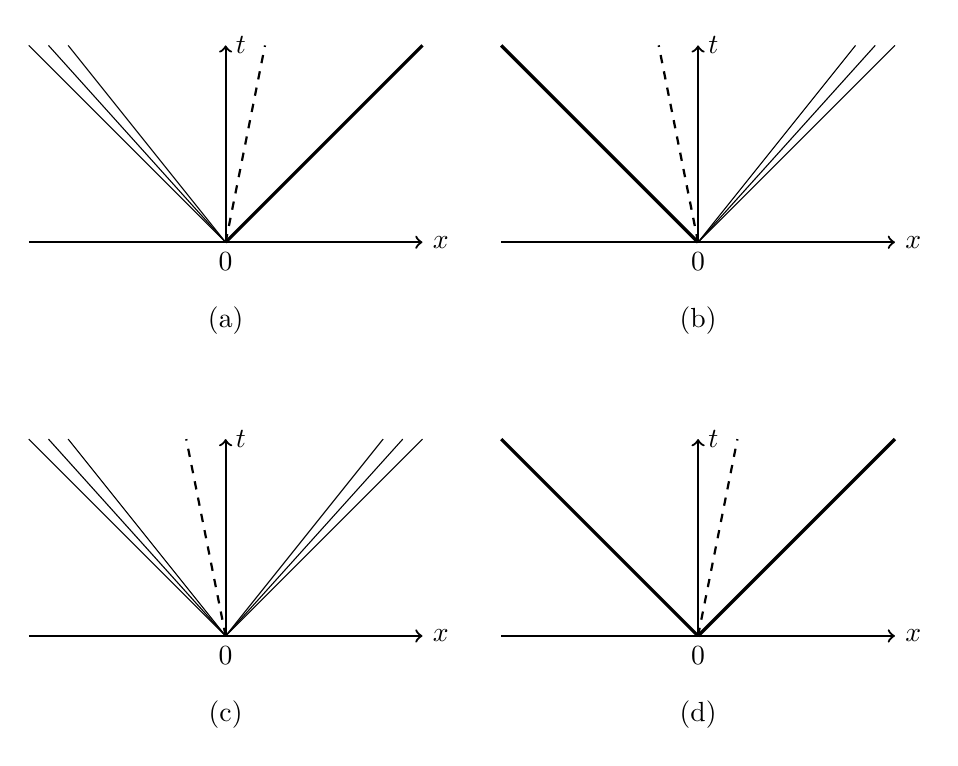
\begin{tikzpicture}[scale=0.25]
		%first
		\draw[thick,->] (-10,0) -- (10,0) node[anchor=west]{$x$};
		\draw[thick,->] (0,0) node[anchor=north]{$0$} -- (0,7) -- (0,9) -- (0,10) node[anchor=west]{$t$};
		\draw[thin,-] (0,0) -- (-10,10);
		\draw[thin,-] (0,0) -- (-9,10);
		\draw[thin,-] (0,0) -- (-8,10);
		\draw[thick,dashed] (0,0) -- (2,10);
		\draw[very thick,-] (0,0) -- (10,10);
		\node at (0,-4) {(a)};
		%second
		\draw[thick,->] (14,0) -- (34,0) node[anchor=west]{$x$};
		\draw[thick,->] (24,0) node[anchor=north]{$0$} -- (24,7) -- (24,9) -- (24,10) node[anchor=west]{$t$};
		\draw[thin,-] (24,0) -- (34,10);
		\draw[thin,-] (24,0) -- (33,10);
		\draw[thin,-] (24,0) -- (32,10);
		\draw[thick,dashed] (24,0) -- (22,10);
		\draw[very thick,-] (24,0) -- (14,10);
		\node at (24,-4) {(b)};
		%third
		\draw[thick,->] (-10,-20) -- (10,-20) node[anchor=west]{$x$};
		\draw[thick,->] (0,-20) node[anchor=north]{$0$} -- (0,-13) -- (0,-11) -- (0,-10) node[anchor=west]{$t$};
		\draw[thin,-] (0,-20) -- (-10,-10);
		\draw[thin,-] (0,-20) -- (-9,-10);
		\draw[thin,-] (0,-20) -- (-8,-10);
		\draw[thick,dashed] (0,-20) -- (-2,-10);
		\draw[thin,-] (0,-20) -- (10,-10);
		\draw[thin,-] (0,-20) -- (9,-10);
		\draw[thin,-] (0,-20) -- (8,-10);
		\node at (0,-24) {(c)};
		%fourth
		\draw[thick,->] (14,-20) -- (34,-20) node[anchor=west]{$x$};
		\draw[thick,->] (24,-20) node[anchor=north]{$0$} -- (24,-13) -- (24,-11) -- (24,-10) node[anchor=west]{$t$};
		\draw[very thick,-] (24,-20) -- (34,-10);
		\draw[thick,dashed] (24,-20) -- (26,-10);
		\draw[very thick,-] (24,-20) -- (14,-10);
		\node at (24,-24) {(d)};
	\end{tikzpicture}
	\caption[Configuration of the wave system: (a) Left rarefaction, contact, right shock. (b) Left shock, contact, right rarefaction. (c) Left rarefaction, contact, right rarefaction. (d) Left shock, contact, right shock.]{Configuration of the wave system: (a) Left rarefaction, contact, right shock. (b) Left shock, contact, right rarefaction. (c) Left rarefaction, contact, right rarefaction. (d) Left shock, contact, right shock.}
	\label{fig:WaveConfig}
\end{figure}
Where, as in the case of \equationref{eqn:RiemannProblem}, the left and right states, $\boldsymbol{W}_L$ and $\boldsymbol{W}_R$, are separated by a discontinuity at $x = 0$. For an ideal gas that obeys the caloric equation of state in \equationref{eqn:idealgasEOS}, the wave system created by the removal of the membrane has four possible configurations of waves seen in \figureref{fig:WaveConfig}. The wave system can consist of left and right rarefaction waves, left and right shock waves or a combination of the two \cite{toro2013riemann}. As can be viewed in \figureref{fig:SolutionStructure}, the left and right waves are separated by a contact discontinuity. The unknown regions between the left and right states are referred to as the star region, which contains the left and right star states, $\boldsymbol{W}_{*L}$ and $\boldsymbol{W}_{*L}$. An iterative solver for the Riemann problem is presented in \sectionref{sect:AdaptiveRiemannSolver}.
\begin{figure}
	\centering
	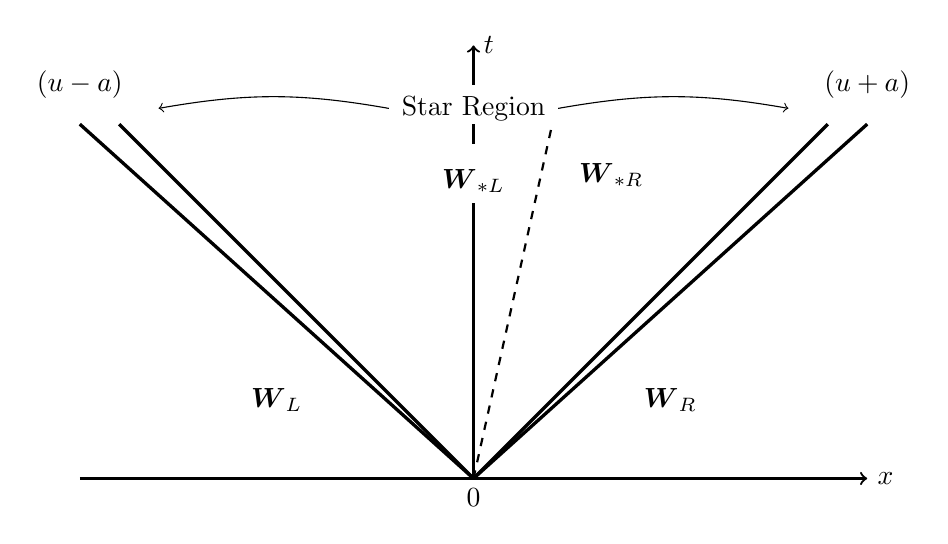
\begin{tikzpicture}[scale=0.5]
		\draw[thick,->] (-10,0) -- (10,0) node[anchor=west]{$x$};
		\draw[thick,-] (0,0)node[anchor=north]{$0$} -- (0,7)node[anchor=south]{$\boldsymbol{W}_{*L}$};
		\draw[thick,-] (0,8.5) -- (0,9);
		\draw[thick,->] (0,10) -- (0,11) node[anchor=west]{$t$};
		\node at (3.5,7.7){$\boldsymbol{W}_{*R}$};
		\draw[very thick,-] (0,0) -- (10,9);
		\draw[very thick,-] (0,0) -- (9,9);
		\draw[thick,dashed] (0,0) -- (2,9);
		\draw[very thick,-] (0,0) -- (-9,9);
		\draw[very thick,-] (0,0) -- (-10,9);
		\node at (-10,10){$\left(u-a\right)$};
		\node at (10,10){$\left(u+a\right)$};
		\node at (-5,2){$\boldsymbol{W}_{L}$};
		\node at (5,2){$\boldsymbol{W}_{R}$};
		\draw[thin,->] (-2.15,9.4) to [out=170,in=10] (-8,9.4);
		\draw[thin,->] (2.15,9.4) to [out=10,in=170] (8,9.4);
		\node at (0,9.4){Star Region};
	\end{tikzpicture}
	\caption[Solution structure of the Riemann problem on the $x$-$t$ plane for the time-dependent Euler equations.]{Solution structure of the Riemann problem on the $x$-$t$ plane for the time-dependent Euler equations.}
	\label{fig:SolutionStructure}
\end{figure}
%\begin{figure}
%\begin{tikzpicture}[scale=0.2]
%\end{tikzpicture}
%\caption[Wave Configuration 2: Left shock wave, centered contact discontinuity, and a right rarefaction wave.]{Wave Configuration 2: Left shock wave, centered contact discontinuity, and a right rarefaction wave.}
%\label{fig:RightTransonicRarefaction}
%\end{figure}
%\begin{figure}
%\begin{tikzpicture}[scale=0.2]
%	\draw[thick,->] (-10,0) -- (10,0) node[anchor=west]{$x$};
%	\draw[thick,->] (0,0) node[anchor=north]{$0$} -- (0,7) -- (0,9) -- (0,10) node[anchor=west]{$t$};
%	\draw[thin,-] (0,0) -- (-10,10);
%	\draw[thin,-] (0,0) -- (-9,10);
%	\draw[thin,-] (0,0) -- (-8,10);
%	\draw[thick,dashed] (0,0) -- (2,10);
%	\draw[thin,-] (0,0) -- (10,10);
%	\draw[thin,-] (0,0) -- (9,10);
%	\draw[thin,-] (0,0) -- (8,10);
%\end{tikzpicture}
%\caption[Wave Configuration 3: Left rarefaction wave, centered contact discontinuity, and a right rarefaction wave.]{Wave Configuration 3: Left rarefaction wave, centered contact discontinuity, and a right rarefaction wave.}
%\label{fig:TwoRarefaction}
%\end{figure}
%\begin{figure}
%\begin{tikzpicture}[scale=0.2]
%	\draw[thick,->] (-10,0) -- (10,0) node[anchor=west]{$x$};
%	\draw[thick,->] (0,0) node[anchor=north]{$0$} -- (0,7) -- (0,9) -- (0,10) node[anchor=west]{$t$};
%	\draw[very thick,-] (0,0) -- (10,10);
%	\draw[thick,dashed] (0,0) -- (-2,10);
%	\draw[very thick,-] (0,0) -- (-10,10);
%\end{tikzpicture}
%\caption[Wave Configuration 4: Left shock wave, centered contact discontinuity, and a right shock wave.]{Wave Configuration 4: Left shock wave, centered contact discontinuity, and a right shock wave.}
%\label{fig:TwoShock}
%\end{figure}
\section{The Approximate Riemann Problem}
For a linear hyperbolic system with constant coefficients, the difference in the conservative variables can be written as
\begin{equation}
	\Delta \boldsymbol{U} = \boldsymbol{U}_R - \boldsymbol{U}_L
\end{equation}
Which when projected onto the right eigenvectors of the Jacobian Matrix, $\tilde{\boldsymbol{A}}$, becomes
\begin{equation}\label{eqn:datadifference}
	\Delta \boldsymbol{U} = \boldsymbol{U}_R - \boldsymbol{U}_L = \sum_{i=1}^m \tilde{\alpha}_i \tilde{\boldsymbol{K}}^{\left(i\right)}
\end{equation}
Where $\tilde{\alpha}_i$ are the associated wave strengths. The values of $\boldsymbol{U}_{i+\frac{1}{2}}$ are evaluated using the equations
\begin{equation}\label{eqn:Usum1}
	\boldsymbol{U}_{i+\frac{1}{2}}\left(0\right) = \boldsymbol{U}_L + \sum_{\tilde{\lambda}_i \le 0} \tilde{\alpha}_i \tilde{\boldsymbol{K}}^{\left(i\right)}
\end{equation}
or from
\begin{equation}\label{eqn:Usum2}
	\boldsymbol{U}_{i+\frac{1}{2}}\left(0\right) = \boldsymbol{U}_R - \sum_{\tilde{\lambda}_i \ge 0} \tilde{\alpha}_i \tilde{\boldsymbol{K}}^{\left(i\right)}
\end{equation}
Replacing the original system of equations, \equationref{eqn:EulerVector1d}, with a modified linear system with constant coefficients, \equationref{eqn:LinEuler}, we have a modified system
\begin{equation}
	\tilde{\boldsymbol{U}}_t + \tilde{\boldsymbol{F}}\left(\tilde{\boldsymbol{U}}\right)_x = \boldsymbol{0}
\end{equation}
with a flux function
\begin{equation}\label{eqn:FluxDef}
	\tilde{\boldsymbol{F}}\left(\tilde{\boldsymbol{U}}\right) = \tilde{\boldsymbol{A}}\tilde{\boldsymbol{U}}
\end{equation}
The corresponding numerical flux, $\boldsymbol{F}$, is found from the following relations
\begin{equation}\label{eqn:flux1}
	\boldsymbol{F}_{0L} = \boldsymbol{F}_L - S_L \boldsymbol{U}_L - \frac{1}{T} \int_{TS_L}^{0} \boldsymbol{U}\left(x,T\right)\,dx
\end{equation}
\begin{equation}\label{eqn:flux2}
	\boldsymbol{F}_{0R} = \boldsymbol{F}_R - S_R \boldsymbol{U}_R + \frac{1}{T} \int_{0}^{TS_R} \boldsymbol{U}\left(x,T\right)\,dx
\end{equation}
Where $S_R$ and $S_L$ are the largest and smallest wave speeds in the exact solution of the Riemann problem that has the right and left states $\boldsymbol{U}_R$ and $\boldsymbol{U}_L$ and $T$ is some positive time. If $\boldsymbol{U}_{i+\frac{1}{2}} \left(x,t\right)$ is a solution of the Riemann problem for the system given in \equationref{eqn:EulerVector1d}, the integral relations in \equationref{eqn:flux1} and \equationref{eqn:flux2} become
\begin{equation}\label{eqn:flux12}
	\int_{TS_L}^{0} \tilde{\boldsymbol{U}}\left(x,T\right)\,dx = T\left[\tilde{\boldsymbol{F}}\left(\boldsymbol{U}_L\right) - \tilde{\boldsymbol{F}}\left(\tilde{\boldsymbol{U}}_{i+\frac{1}{2}}\right)\right] - T S_L \boldsymbol{U}_L
\end{equation}
\begin{equation}\label{eqn:flux22}
	\int_{0}^{TS_R} \tilde{\boldsymbol{U}}\left(x,T\right)\,dx = T\left[\tilde{\boldsymbol{F}}\left(\tilde{\boldsymbol{U}}_{i+\frac{1}{2}}\right) - \tilde{\boldsymbol{F}}\left(\boldsymbol{U}_R\right)\right] + T S_R \boldsymbol{U}_R
\end{equation}
Substituting \equationref{eqn:flux12} and \equationref{eqn:flux22} into \equationref{eqn:flux1} and \equationref{eqn:flux2} gives the following
\begin{equation}\label{eqn:flux13}
	\boldsymbol{F}_{0L} = \tilde{\boldsymbol{F}}\left(\tilde{\boldsymbol{U}}_{i+\frac{1}{2}}\left(0\right)\right) + \boldsymbol{F}\left(\boldsymbol{U}_L\right) - \tilde{\boldsymbol{F}}\left(\boldsymbol{U}_L\right)
\end{equation}
\begin{equation}\label{eqn:flux23}
	\boldsymbol{F}_{0R} = \tilde{\boldsymbol{F}}\left(\tilde{\boldsymbol{U}}_{i+\frac{1}{2}}\left(0\right)\right) + \boldsymbol{F}\left(\boldsymbol{U}_R\right) - \tilde{\boldsymbol{F}}\left(\boldsymbol{U}_R\right)
\end{equation}
Using $\tilde{\boldsymbol{U}}_{i+\frac{1}{2}}\left(0\right)$ from \equationref{eqn:Usum1} or from \equationref{eqn:Usum2} and using \equationref{eqn:FluxDef} the numerical flux is given by
\begin{equation}\label{eqn:Fsum1}
	\boldsymbol{F}_{i+\frac{1}{2}} = \boldsymbol{F}_L + \sum_{\tilde{\lambda}_i \le 0} \tilde{\alpha}_i  \tilde{\lambda}_i  \tilde{\boldsymbol{K}}^{\left(i\right)}
\end{equation}
or from
\begin{equation}\label{eqn:Fsum2}
	\boldsymbol{F}_{i+\frac{1}{2}} = \boldsymbol{F}_R - \sum_{\tilde{\lambda}_i \ge 0} \tilde{\alpha}_i  \tilde{\lambda}_i  \tilde{\boldsymbol{K}}^{\left(i\right)}
\end{equation}
The simple arithmetic average of the numerical flux definitions of \equationref{eqn:Fsum1} and \equationref{eqn:Fsum2} used in the computation is
\begin{equation}\label{eqn:NumericalFluxAverage}
	\boldsymbol{F}_{i+\frac{1}{2}} = \frac{1}{2} \left( \boldsymbol{F}_L + \boldsymbol{F}_R \right)- \frac{1}{2}\sum_{i = 1}^{m} \tilde{\alpha}_i  |\tilde{\lambda}_i |  \tilde{\boldsymbol{K}}^{\left(i\right)}
\end{equation}
\chapter{Riemann Solvers}\label{ch:NumericalMethods}
\section{Finite Volume Method}

The method used to discretize the one-dimensional Euler equations is the Finite Volume Method. The Finite Volume Method approximates the value at the cell centers by using the flux across the cell faces. Integrating \equationref{eqn:LinEuler} over space
\begin{equation}
	\int_V \boldsymbol{U}_t dV + \int_V \boldsymbol{F}_xdV = \boldsymbol{0}
\end{equation}
and using the Gauss-Divergence Theorem the Volume integral over the flux term can be converted to a surface integral.
\begin{equation}
	\int_V \left(\nabla \boldsymbol{\cdot} \boldsymbol{F}\right) dV = \int_S \boldsymbol{F} \boldsymbol{\cdot} d\hat{A}
\end{equation}
Converting the integral of the flux vector, $\boldsymbol{F}$, into a surface integral gives the following
\begin{equation}
	\int_V \boldsymbol{U}_t\,dV + \int_S  \boldsymbol{F} \boldsymbol{\cdot} \boldsymbol{\hat{n}}\,dS = \boldsymbol{0}
\end{equation}
The surface integral can then be represented as a sum over the surface area of the faces of a cell denoted as seen in \figureref{fig:CellSetUp}. In one dimension this reduces to
\begin{equation}\label{eqn:spatiallydiscretized}
	\boldsymbol{U}_t \Delta x + \left[\boldsymbol{F}_{i+\frac{1}{2}} - \boldsymbol{F}_{i-\frac{1}{2}}\right] = \boldsymbol{0}
\end{equation}
The spatially discretized equation can then be represented as
\begin{equation}\label{eqn:spatiallydiscretized2}
	\boldsymbol{U}_t = - \frac{1}{\Delta x} \left[\boldsymbol{F}_{i+\frac{1}{2}} - \boldsymbol{F}_{i-\frac{1}{2}}\right]
\end{equation}
\equationref{eqn:spatiallydiscretized2} can then be solved by finding the value of the numerical flux and an appropriate time discretization.
\begin{figure}
	\centering
	\begin{tikzpicture}[scale=1]
		\draw[thick,->] (-3,0) -- (8,0)node[anchor=west]{$x$};
		\draw[thin,dashed] (1,-1) -- (1,1);
		\draw[thin,dashed] (4,-1) -- (4,1);
		\draw[thin,dashed] (7,-1) -- (7,1);
		\draw[thin,dashed] (-2,-1) -- (-2,1);
		\node[circle,draw=black, fill=white, inner sep=0pt,minimum size=5pt] (b) at (2.5,0) {};
		\node[circle,draw=black, fill=white, inner sep=0pt,minimum size=5pt] (b) at (5.5,0) {};
		\node[circle,draw=black, fill=white, inner sep=0pt,minimum size=5pt] (b) at (-0.5,0) {};
		\node at (2.5,-0.5) {$i$};
		\node at (5.5,-0.5) {$i+1$};
		\node at (-0.5,-0.5) {$i-1$};
		\node at (4,-1.5) {$i+\frac{1}{2}$};
		\node at (1,-1.5) {$i-\frac{1}{2}$};
		\node at (-2,-1.5) {$i-\frac{3}{2}$};
		\node at (7,-1.5) {$i+\frac{3}{2}$};
		\draw[thick,->] (5,1.5) to [out=270,in=30] (4,1.1);
		\node at (5,1.75) {Cell Face};
		\node at (2.5,1.75) {Cell Center};
		\draw[thick,->] (2.5,1.5) to [out=270,in=90] (2.5,0.15);
	\end{tikzpicture}
	\caption[Cell Configuration for a one-dimensional grid.]{Cell Configuration for a one-dimensional grid.}
	\label{fig:CellSetUp}
\end{figure}
\section{Roe's Approximate Riemann Solver}

Roe \cite{ROE1997250} presented an approximate Riemann solver that uses an averaged Jacobian matrix, the Roe matrix $\tilde{\boldsymbol{A}}$, from which $\tilde{\lambda}_i$, $\tilde{\boldsymbol{K}}^{(i)}$, and $\tilde{\alpha}_i$ of \equationref{eqn:NumericalFluxAverage} can be found directly. This direct approximation to the flux function, $\boldsymbol{F}_{i+\frac{1}{2}}$, avoided the pressure iterations of Godunov's method, decreasing the computation time. Roe's breakthrough in constructing $\tilde{\boldsymbol{A}}$ was the introduction of a parameter vector, $\boldsymbol{Q}$, such that both $\boldsymbol{U}$ and $\boldsymbol{F}\left(\boldsymbol{U}\right)$ could be expressed in terms of $\boldsymbol{Q}$ \cite{toro2013riemann}. Roe starts by choosing the parameter vector, $\boldsymbol{Q}$ as
\begin{equation}
	\boldsymbol{Q} = \begin{bmatrix}
		q_1\\ q_2\\ q_3
	\end{bmatrix} = \sqrt{\rho} \begin{bmatrix}
		1\\ u\\ H
	\end{bmatrix}
\end{equation}
The differences in the data of $\boldsymbol{Q}$ are now expressed in terms of an averaged vector, $\tilde{\boldsymbol{Q}}$, which is found by a simple arithmetic average of the left and right states of $\boldsymbol{Q}$.
\begin{equation}
	\tilde{\boldsymbol{Q}} = \frac{1}{2} \left(\boldsymbol{Q}_L + \boldsymbol{Q}_R\right)
\end{equation}
Two Matrices are found, $\tilde{\boldsymbol{B}}$ and $\tilde{\boldsymbol{C}}$, so that the differences in the data, $\Delta \boldsymbol{U}$ and $\Delta \boldsymbol{F}$, can be expressed as
\begin{equation}
	\Delta \boldsymbol{U} = \tilde{\boldsymbol{B}} \Delta \boldsymbol{Q} ; \,\,\,\, \Delta \boldsymbol{F} = \tilde{\boldsymbol{C}} \Delta \boldsymbol{Q}
\end{equation}
$\tilde{\boldsymbol{B}}$ and $\tilde{\boldsymbol{C}}$ have the following form
\begin{equation}
	\tilde{\boldsymbol{B}} = \begin{bmatrix}
		2\tilde{q}_1 & 0 & 0\\
		\tilde{q}_2 & \tilde{q}_1 & 0\\
		\frac{\tilde{q}_3}{\gamma} & \frac{\gamma-1}{\gamma}\tilde{q}_2 & \frac{\tilde{q}_1}{\gamma}
	\end{bmatrix}
\end{equation}
\begin{equation}
	\tilde{\boldsymbol{C}} = \begin{bmatrix}
		\tilde{q}_2 & \tilde{q}_1 & 0\\
		\frac{\gamma-1}{\gamma}\tilde{q}_3 & \frac{\gamma-1}{\gamma}\tilde{q}_2 & \frac{\gamma-1}{\gamma}\tilde{q}_1\\
		0 & \tilde{q}_3 & \tilde{q}_2
	\end{bmatrix}
\end{equation}
The Roe matrix, $\tilde{\boldsymbol{A}}$, can then be expressed as
\begin{equation}
	\tilde{\boldsymbol{A}} = \tilde{\boldsymbol{B}} \tilde{\boldsymbol{C}}^{-1}
\end{equation}
Which has the eigenvalues
\begin{equation}
	\tilde{\lambda}_1 = \tilde{u} - \tilde{a},\,\,\,\,\tilde{\lambda}_2 = \tilde{u},\,\,\,\,\tilde{\lambda}_3 = \tilde{u} + \tilde{a}
\end{equation}
and the corresponding right eigenvectors
\begin{equation}\label{eq:eigenvectors}
	\tilde{\boldsymbol{K}}^{\left(1\right)} = \begin{bmatrix}
		1 \\ \tilde{u} - \tilde{a} \\ \tilde{H} - \tilde{u} \tilde{a}
	\end{bmatrix},\,\,\,\,
	\tilde{\boldsymbol{K}}^{\left(2\right)} = \begin{bmatrix}
		1 \\ \tilde{u} \\ \frac{1}{2} \tilde{u}^2
	\end{bmatrix},\,\,\,\,
	\tilde{\boldsymbol{K}}^{\left(3\right)} = \begin{bmatrix}
		1 \\ \tilde{u} + \tilde{a} \\ \tilde{H} + \tilde{u} \tilde{a}
	\end{bmatrix}
\end{equation}
The Roe averaged variables, $\tilde{u}$, $\tilde{H}$, and $\tilde{a}$, are calculated as follows
\begin{equation}
	\tilde{u} = \frac{\sqrt{\rho_L} u_L + \sqrt{\rho_R} u_R}{\sqrt{\rho_L} + \sqrt{\rho_R}}
\end{equation}
\begin{equation}
	\tilde{H} = \frac{\sqrt{\rho_L} H_L + \sqrt{\rho_R} H_R}{\sqrt{\rho_L} + \sqrt{\rho_R}}
\end{equation}
\begin{equation}
	\tilde{a} = \left[\left(\gamma - 1\right) \left(\tilde{H} - \frac{1}{2} \tilde{u}^2\right)\right]^{\frac{1}{2}}
\end{equation}
Using the definition of the data difference from \equationref{eqn:datadifference} a set of equations is obtained, that when solved allow the computation of the numerical flux.
\begin{equation}
	\tilde{\alpha}_1 + \tilde{\alpha}_2 + \tilde{\alpha}_3 = \Delta u_1
\end{equation}
\begin{equation}
	\tilde{\alpha}_1 \left(\tilde{u} - \tilde{a}\right) + \tilde{\alpha}_2 \tilde{u} + \tilde{\alpha}_3 \left(\tilde{u} + \tilde{a}\right) = \Delta u_2
\end{equation}
\begin{equation}
	\tilde{\alpha}_1 \left(\tilde{H} - \tilde{u}\tilde{a}\right) + \frac{1}{2} u^2 \tilde{\alpha}_2 + \tilde{\alpha}_3 \left(\tilde{H} + \tilde{u}\tilde{a}\right) = \Delta u_3
\end{equation}
Solving these equations for the wave strengths, it can be found that
\begin{equation}
	\tilde{\alpha}_2 = \frac{\gamma - 1}{\tilde{a}^2} \left[\Delta u_1 \left(\tilde{H} - \tilde{u}^2\right)  + \tilde{u} \Delta u_2 - \Delta u_3\right]
\end{equation}
\begin{equation}
	\tilde{\alpha}_1 = \frac{1}{2 \tilde{a}} \left[\Delta u_1\left(\tilde{u} + \tilde{a}\right) - \Delta u_2 - \tilde{a}\tilde{\alpha}_2\right]
\end{equation}
\begin{equation}\label{eq:wavestrength3}
	\tilde{\alpha}_3 = \Delta u_1 - \left(\tilde{\alpha}_1 + \tilde{\alpha}_2\right)
\end{equation}
So that the numerical flux may be calculated as described in \equationref{eqn:NumericalFluxAverage}.

The Roe numerical flux can also be expressed in terms of the Roe matrix $\boldsymbol{\tilde{A}}$. Letting $\boldsymbol{\tilde{\Lambda}}$ be the matrix of eigenvalues of the Roe matrix
\begin{equation}
	\boldsymbol{\tilde{\Lambda}} = \begin{bmatrix}
		\tilde{u} - \tilde{a} & 0 & 0 \\
		0 & \tilde{u} & 0 \\
		0 & 0 & \tilde{u} + \tilde{a}
	\end{bmatrix}
\end{equation}
and $\boldsymbol{\tilde{K}}$ be the matrix of right eigenvectors
\begin{equation}
	\boldsymbol{\tilde{K}} = \begin{bmatrix}
		1 & 1 & 1 \\
		\tilde{u}-\tilde{a} & \tilde{u} & \tilde{u}+\tilde{a} \\
		\tilde{H}-\tilde{u}\tilde{a} & \frac{1}{2} \tilde{u}^2 & \tilde{H}+\tilde{u}\tilde{a}
	\end{bmatrix}
\end{equation}
then the matrix $|\boldsymbol{\tilde{A}}|$ is given by
\begin{equation}
	|\boldsymbol{\tilde{A}}| = \boldsymbol{\tilde{K}} |\boldsymbol{\tilde{\Lambda}}| \boldsymbol{\tilde{K}}^{-1}
\end{equation}
then the Roe flux in matrix form is
\begin{equation}
	\boldsymbol{\tilde{F}}_{i+\frac{1}{2}} = \frac{1}{2}\left(\boldsymbol{F}_L + \boldsymbol{F}_R\right) - \frac{1}{2} |\boldsymbol{\tilde{A}}| \left(\boldsymbol{U}_R - \boldsymbol{U}_L\right)
\end{equation}
%\begin{equation}
%	\boldsymbol{\tilde{F}}_{i+\frac{1}{2}} = \frac{1}{2}\left(\boldsymbol{F}_L + \boldsymbol{F}_R\right)_{i+\frac{1}{2}} - \frac{1}{2} |\boldsymbol{\tilde{A}}|_{i+\frac{1}{2}} \left(\boldsymbol{U}_R - \boldsymbol{U}_L\right)_{i+\frac{1}{2}}
%\end{equation}
%\begin{equation}
%\boldsymbol{\tilde{F}}_{i-\frac{1}{2}} = \frac{1}{2}\left(\boldsymbol{F}_L + \boldsymbol{F}_R\right)_{i-\frac{1}{2}} - \frac{1}{2} |\boldsymbol{\tilde{A}}|_{i-\frac{1}{2}} \left(\boldsymbol{U}_R - \boldsymbol{U}_L\right)_{i-\frac{1}{2}}
%\end{equation}
%\begin{equation}\label{eq:eigenvectors}
%	\tilde{\boldsymbol{K}}^{\left(1\right)} = \begin{bmatrix}
%		1 \\ \tilde{u} - \tilde{a} \\ \tilde{H} - \tilde{u} \tilde{a}
%	\end{bmatrix},\,\,\,\,
%	\tilde{\boldsymbol{K}}^{\left(2\right)} = \begin{bmatrix}
%		1 \\ \tilde{u} \\ \frac{1}{2} \tilde{u}^2
%	\end{bmatrix},\,\,\,\,
%	\tilde{\boldsymbol{K}}^{\left(3\right)} = \begin{bmatrix}
%		1 \\ \tilde{u} + \tilde{a} \\ \tilde{H} + \tilde{u} \tilde{a}
%	\end{bmatrix}
%\end{equation}
Roe's scheme has two difficulties. Firstly, the scheme needs a correction to avoid the appearance of entropy violating shocks discussed in \sectionref{sect:EntropyFix}. Second, the scheme also fails near low-density flows. Roe's method fails near low densities because the wave speeds are underestimated and can lead to solutions that include negative pressures and densities. Einfeldt, Munz, Roe, and Sjögreen \cite{EINFELDT1991273} proved that this vacuum problem affects all linearized Riemann solvers.
\section{Harten-Hyman Entropy Fix}\label{sect:EntropyFix}
Roe's Approximate Riemann solver leads to the development of entropy violating shocks within rarefaction waves, sometimes called rarefaction shocks \cite{toro2013riemann}. These rarefaction shocks occur when the eigenvalues of the Jacobian matrix vanish in sonic regions \cite{Kermani}. In practical computations, the entropy violating discontinuous waves cause difficulties when the rarefaction wave is transonic \cite{toro2013riemann}. There are then have two cases where these unphysical shocks occur --- in left and right transonic rarefactions. Modifications to Roe's Riemann solver can be made to avoid these entropy violating shocks. Harten and Hyman \cite{HARTEN1983235} suggested an entropy fix that has gained widespread use. Toro's \cite{toro2013riemann} formulation of the Harten and Hyman entropy fix for the time-dependent Euler equations is discussed here.

\subsection{Left Transonic Rarefaction}

In the case of a left transonic rarefaction the wave speeds are calculated as follows
\begin{equation}
	\lambda_1^L = u_L - a_L ; \, \, \lambda_1^R = u_* - a_{*L}
\end{equation}
where $u_*$ and $a_*$ are calculated from $\boldsymbol{U}_{*L}$ and $\boldsymbol{U}_{*R}$ found in \sectionref{sect:AdaptiveRiemannSolver}. If
\begin{equation}
	\lambda_1^L < 0 < \lambda_1^R
\end{equation}
then the left wave is a transonic rarefaction wave and the entropy fix is enforced in the following way. The single jump
\begin{equation}\label{eqn:SingleJump1}
	\boldsymbol{U}_{*L} - \boldsymbol{U}_L = \tilde{\alpha}_1 \tilde{\boldsymbol{K}}^{(1)}
\end{equation}
is a wave traveling with a speed $\tilde{\lambda}_1$ and is split into two smaller data jumps $\boldsymbol{U}_{SL} - \boldsymbol{U}_L$ and $\boldsymbol{U}_{*L} - \boldsymbol{U}_{SL}$. The jumps are traveling at speeds $\lambda_1^L$ and $\lambda_1^R$ respectively and $\boldsymbol{U}_{SL}$ is a transonic state that is to be found. Using \equationref{eq:IntegralForm} the following is found
\begin{equation}\label{eq:IntegralEvaluated}
	\lambda_1^R \left(\boldsymbol{U}_{SL} - \boldsymbol{U}_{*L}\right) + \lambda_1^L \left(\boldsymbol{U}_{L} - \boldsymbol{U}_{SL}\right) = \tilde{\lambda}_1 \left(\boldsymbol{U}_{L} - \boldsymbol{U}_{*L}\right)
\end{equation}
$\boldsymbol{U}_{SL}$ can then be found by
\begin{equation}
	\boldsymbol{U}_{SL} = \frac{ \left( \tilde{\lambda}_1 - \lambda_1^L \right) \boldsymbol{U}_L + \left( \tilde{\lambda}_1 - \lambda_1^R \right) \boldsymbol{U}_{*L}}{\lambda_1^R - \lambda_1^L}
\end{equation}
Using the one-sided Roe flux from \equationref{eqn:Fsum1} and applying to \equationref{eq:IntegralEvaluated}, the data jump $\boldsymbol{U}_{SL} - \boldsymbol{U}_L$ can be expressed as
\begin{equation}
	\boldsymbol{U}_{SL} - \boldsymbol{U}_L = \frac{\left( \lambda_1^R - \tilde{\lambda}_1 \right)}{\left(\lambda_1^R - \lambda_1^L\right)} \left(\boldsymbol{U}_{*L} - \boldsymbol{U}_L\right)
\end{equation}
The Roe approximation from \equationref{eqn:SingleJump1} leads to the flux jump $\left(\Delta \boldsymbol{F}\right)_1^L$ across the wave of speed $\lambda_1^L$ to be
\begin{equation}
	\left(\Delta \boldsymbol{F}\right)_1^L = \lambda_1^L \left(\frac{\lambda_1^R - \tilde{\lambda}_1}{\lambda_1^R - \lambda_1^L}\right) \tilde{\alpha}_1 \tilde{\boldsymbol{K}}^{(1)}
\end{equation}
A new wave speed, $\bar{\lambda}_1$, can then be defined as
\begin{equation}
	\bar{\lambda}_1 = \lambda_1^L \left(\frac{\lambda_1^R - \tilde{\lambda}_1}{\lambda_1^R - \lambda_1^L}\right)
\end{equation}
so that the intercell flux from \equationref{eqn:Fsum1} is now
\begin{equation}\label{eq:Fsum1Entropy}
	\boldsymbol{F}_{i+\frac{1}{2}} = \boldsymbol{F}_L + \bar{\lambda}_1 \tilde{\alpha}_1 \tilde{\boldsymbol{K}}^{(1)}
\end{equation}
\subsection{Right Transonic Rarefaction}
In the case of a right transonic rarefaction we can define two new wave speeds in the same manner as the left case.
\begin{equation}
	\lambda_3^L = u_* + a_{*R} ; \, \, \lambda_3^R = u_R + a_R
\end{equation}
If
\begin{equation}
	\lambda_3^L < 0 < \lambda_3^R
\end{equation}
then the right wave is a transonic rarefaction wave and the transonic state $\boldsymbol{U}_{SR}$ between the waves of speeds $\lambda_3^L$ and $\lambda_3^R$ is given as
\begin{equation}
	\boldsymbol{U}_{SR} = \frac{ \left( \lambda_3^R - \tilde{\lambda_3} \right) \boldsymbol{U}_R + \left( \tilde{\lambda}_3 - \lambda_3^L \right) \boldsymbol{U}_{*R}}{\lambda_3^R - \lambda_3^L}
\end{equation}
A new wave speed, $\bar{\lambda}_3$, can then be defined as
\begin{equation}
	\bar{\lambda}_3 = \lambda_3^R \left(\frac{\tilde{\lambda}_3 - \lambda_3^R}{\lambda_3^R - \lambda_3^L}\right)
\end{equation}
Using the one-sided Roe flux from \equationref{eqn:Fsum2} and applying this new wave speed we have
\begin{equation}\label{eq:Fsum2Entropy}
	\boldsymbol{F}_{i+\frac{1}{2}} = \boldsymbol{F}_R - \bar{\lambda}_3 \tilde{\alpha}_1 \tilde{\boldsymbol{K}}^{(3)}
\end{equation}
Taking the simple average of \equationref{eq:Fsum1Entropy} and \equationref{eq:Fsum2Entropy} we again arrive at \equationref{eqn:NumericalFluxAverage} as the centered formula for the Roe flux.

\section{Adaptive Riemann Solver}\label{sect:AdaptiveRiemannSolver}

In order to find the speeds $u_*$, $a_{*L}$, and $a_{*R}$, $\boldsymbol{U}_{*R}$ and $\boldsymbol{U}_{*L}$ need to be found. Toro \cite{toro2013riemann} provides an adaptive Riemann solver outlined here that has been modified to include an iterative scheme to find the star states. The adaptive Riemann solver starts by defining a switching parameter $Q_{user}$ and a switching condition parameter $Q$ defined as
\begin{equation}
	Q = \frac{p_{max}}{p_{min}}
\end{equation}
and the $p_*$ state taken from the Primitive Variable Riemann Solver (PVRS) of \sectionref{sect:PVRS} as
\begin{equation}
	p_* = p_{pvrs}
\end{equation}
A choice of $Q_{user} = 2$ results in robust and efficient schemes that can handle most Riemann problems \cite{toro2013riemann}. If
\begin{equation}
	Q < Q_{user}
\end{equation}
and
\begin{equation}
	p_{min} < p_* < p_{max}
\end{equation}
then the PVRS is used for the star state calculations. If
\begin{equation}
	p_* < p_{min}
\end{equation}
then the Two Rarefaction Riemann Solver (TRRS) of \sectionref{sect:TRRS} is used. If none of the conditions is met then the Two Shock Riemann Solver (TSRS) of \sectionref{sect:TSRS} is used for the star state calculations. In all cases, the value of $p_*$ is an initial guess for the following Iterative Riemann Solver (IRS) using the Newton-Raphson method.

\begin{equation}
	f_k = \begin{cases}
		\left(p_* - p\right) \sqrt{\frac{A_k}{p_* + B_k}} \,\,\,\, \textrm{if} \,\,\,\, p_* > p \,\,\,\, \left(\textrm{shock}\right)\\
		\frac{2 a_k}{\gamma - 1} \left(\frac{p_*}{p}\right)^{\frac{\gamma - 1}{2 \gamma - 1}}\,\,\,\, \textrm{if} \,\,\,\, p_* \le p \,\,\,\, \left(\textrm{rarefaction}\right)
	\end{cases}
\end{equation}
\begin{equation}
	f^{\prime}_k = \begin{cases}
		\sqrt{\frac{A_k}{p_* + B_k}} \left[1 - \frac{p_* - p}{ 2 \left(B_k + p\right)}\right]  \,\,\,\, \textrm{if} \,\,\,\, p_* > p \,\,\,\, \left(\textrm{shock}\right)\\
		\frac{1}{\rho_k a_k} \left(\frac{p_*}{p}\right)^{-\frac{\gamma + 1}{2 \gamma}} \,\,\,\, \textrm{if} \,\,\,\, p_* \le p \,\,\,\, \left(\textrm{rarefaction}\right)
	\end{cases}
\end{equation}
Where $A_k$, $B_k$, and $a_k$ are
\begin{equation}
	A_k = \frac{2}{\rho_k \left(\gamma + 1\right)}
\end{equation}
\begin{equation}
	B_k = p \frac{\gamma - 1}{\gamma + 1}
\end{equation}
\begin{equation}
	a_k = \sqrt{\frac{\gamma p}{\rho_k}}
\end{equation}
then $f$ and $f^{\prime}$ are
\begin{equation}
	f = f_L + f_R \,\,\,\, ; f^{\prime} = f^{\prime}_L + f^{\prime}_R
\end{equation}
The Newton-Raphson scheme for an iteration $n$ is then
\begin{equation}
	p_{*,n+1} = p_{*,n-1} - \frac{f_n}{f^{\prime}_n}
\end{equation}
The wave speeds can then be calculated according to the PVRS, TRRS, or TSRS. In the case where the TRRS or TSRS is used, and the wave system is a two rarefaction or two shock system, respectively, the $p_*$ equations are exact and will result in only one iteration.

\tikzstyle{startstop} = [rectangle, rounded corners, minimum width=3cm, minimum height=1cm,text centered, draw=black, fill=red!30]
\tikzstyle{io} = [trapezium, trapezium left angle=70, trapezium right angle=110, minimum width=0.5cm, minimum height=0.5cm, text centered, draw=black, fill=blue!30]
\tikzstyle{process} = [rectangle, minimum width=2cm, minimum height=1cm, text centered, draw=black, fill=orange!30]
\tikzstyle{decision} = [diamond, aspect=3, minimum width=1cm, minimum height=0.5cm, text centered, draw=black, fill=green!30]
\tikzstyle{line} = [draw, -stealth, thick]


\begin{figure}
	\centering
	\begin{tikzpicture}[node distance=1.5cm]
		\node[align=center] (startblock) [startstop] {$Q = \frac{p_{max}}{p_{min}}$ \\ $p_* = p_{pvrs}$};
		\node[align=center] (quser) [decision, below of=startblock,yshift=-1em]{$Q < Q_{user}$ \\ $p_{min} < p_* < p_{max}$};
		\node[align=center] (PVRS) [process, below of=quser,xshift=-10em,yshift=-4.8em]{PVRS};
		\node[align=center] (pmin) [decision, below of=quser,xshift=10em]{$p_* < p_{min}$};
		\node[align=center] (TRRS) [process, below of=pmin,xshift=-5em]{TRRS};
		\node[align=center] (TSRS) [process, below of=pmin,xshift=5em]{TSRS};
		\node[align=center] (IRS) [process, below of=TRRS,xshift=-5em]{IRS};
		\node[align=center] (wave) [startstop,below of=IRS]{Calculate Wave Speed};
		
		\path[line] (startblock.south) -- (quser);
		\path[line] (quser.west) -| node[anchor=south]{\tiny True} (PVRS);
		\path[line] (quser.east) -| node[anchor=south]{\tiny False} (pmin);
		\path[line] (pmin.west) -| node[anchor=east]{\tiny True} (TRRS);
		\path[line] (pmin.east) -| node[anchor=west]{\tiny False} (TSRS);
		\path[line] (TRRS.west) -| (IRS);
		\path[line] (TSRS.south) |- (IRS);
		\path[line] (PVRS.south) |- (IRS);
		\path[line] (IRS.south) -- (wave);
%		\path[line] (roeflux.south) -- + (0,-1em) -| (AvgFlux);
%		\path[line] (roeflux.south) -- + (0,-1em) -| (DiffFlux);
%		\path[line] (AvgFlux.south) -- + (0,-1em) -| (Interface);
%		\path[line] (AvgFlux.south) -- + (0,-1em) -| (CellCenter);
%		\path[line] (DiffFlux.south) -- + (0,-1em) -| (Roe2);
%		\path[line] (DiffFlux.south) -- + (0,-1em) -| (MUSCL2);
%		\path[line] (DiffFlux.south) -- + (0,-1em) -| (WENO32);
%		\path[line] (DiffFlux.south) -- + (0,-1em) -| (WENO52);
%		\path[line] (Interface.south) -- + (0,-1em) -| (Roe1);
%		\path[line] (Interface.south) -- + (0,-1em) -| (MUSCL1);
%		\path[line] (Interface.south) -- + (0,-1em) -| (WENO31);
%		\path[line] (Interface.south) -- + (0,-1em) -| (WENO51);
%		\path[line] (CellCenter.south) -- + (0,-1em) -| (CD2);
%		\path[line] (CellCenter.south) -- + (0,-1em) -| (CD4);
%		\path[line] (CellCenter.south) -- + (0,-1em) -| (CD6);
	\end{tikzpicture}
	\caption[Flowchart for the Adaptive Riemann Solver.]{Flowchart for the Adaptive Riemann Solver.}
	\label{fig:ARSFlowChart}
\end{figure}

%\begin{figure}
%	\centering
%	\begin{tikzpicture}[scale=0.5]
%		\draw[thin,-] (-5,10) -- (5,10) -- (5,7) -- (-5,7) -- (-5,10);
%		\node at (-3,8.5){$Q = \frac{p_{max}}{p_{min}} \,\, ;$};
%		\node at (3,8.5){$p_* = p_{pvrs}$};
%		\draw[thin,->] (0,7) -- (0,6);
%		\draw[thin,-] (0,6) -- (5,4) -- (0,2) -- (-5,4) -- (0,6);
%		\node at (0,4.75) {$Q < Q_{user}$};
%		\node at (0,3.75) {$p_{min} < p_* < p_{max}$};
%		\draw[thin,->] (-5,4) -- (-10,4) -- (-10,-2);
%		\draw[thin,->] (5,4) -- (7.5,4) -- (7.5, 2);
%		\draw[thin,-] (7.5,2) -- (10,0.5) -- (7.5,-1) -- (5,0.5) -- (7.5,2);
%		\node at (7.5,0.5){$p_* < p_{min}$};
%		\draw[thin,->] (10,0.5) -- (12,0.5) -- (12,-2);
%		\draw[thin,->] (5,0.5) -- (3,0.5) -- (3,-2);
%		\draw[thin,-] (-12,-2) -- (-12,-4) -- (-8,-4) -- (-8,-2) -- (-12,-2);
%		\node at (-10,-3) {PVRS};
%		\draw[thin,-] (14,-2) -- (14,-4) -- (10,-4) -- (10,-2) -- (14,-2);
%		\node at (12,-3) {TSRS};
%		\draw[thin,-] (1,-2) -- (1,-4) -- (5,-4) -- (5,-2) -- (1,-2);
%		\node at (3,-3) {TRRS};
%		\draw[thin,->] (-10,-4) -- (-10,-6) -- (-2,-6);
%		\draw[thin,->] (12,-4) -- (12,-6) -- (2,-6);
%		\draw[thin,->] (1,-3) -- (0,-3) -- (0,-5);
%		\draw[thin,-] (0,-5) -- (-2,-5) -- (-2,-7) -- (2,-7) -- (2,-5) -- (0,-5);
%		\node at (0,-6) {IRS};
%	\end{tikzpicture}
%	\caption[Flow Chart for the Adaptive Riemann Solver.]{Flow Chart for the Adaptive Riemann Solver.}
%	\label{fig:ARSFlowChart}
%\end{figure}

\subsection{Primitive Variable Riemann Solver}\label{sect:PVRS}

To estimate the wave speeds using the PVRS, the following star states are calculated
\begin{equation}\label{eq:PVRS}
	\begin{rcases}
		p_* = \frac{1}{2} \left(p_L + p_R\right) + \frac{1}{2} \left(u_L - u_R\right) \bar{\rho} \bar{a}\\
		u_* = \frac{1}{2} \left(u_L + u_R\right) + \frac{1}{2} \left(p_L - p_R\right) / \left(\bar{\rho} \bar{a}\right)\\
		p_{*L} = \rho_L - \left(u_L - u_*\right)\bar{\rho} / \bar{a}\\
		p_{*R} = \rho_R - \left(u_* - u_R\right)\bar{\rho} / \bar{a}
	\end{rcases}
\end{equation}
where $\bar{\rho}$ and $\bar{a}$ are
\begin{equation}
	\bar{\rho} = \frac{1}{2} \left(\rho_L + \rho_R\right) \, , \,\,\,\, \bar{a} = \frac{1}{2} \left(a_L + a_R\right)
\end{equation}
the speeds of sound are calculated as
\begin{equation}
	a_{*L} = \sqrt{\frac{\gamma p_*}{\rho_{*L}}}
\end{equation}
\begin{equation}
	a_{*R} = \sqrt{\frac{\gamma p_*}{\rho_{*R}}}
\end{equation}
\subsection{Two Rarefaction Riemann Solver}\label{sect:TRRS}
To estimate the wave speeds using the TRRS, the initial guess for the pressure $p_*$ is calculated according to
\begin{equation}
	p_* = \left[\frac{a_L + a_R - \frac{\gamma - 1}{2} \left(u_R - u_L\right)}{a_L / p_L^z + a_R / p_R^z}\right]^{\frac{1}{z}}
\end{equation}
where $z$ is given by
\begin{equation}
	z = \frac{\gamma - 1}{2 \gamma}
\end{equation}
the speeds of sound and the particle velocities in the star region are given by
\begin{equation}
	a_{*L} = a_L \left(p_* / p_L\right)^z \, , \,\,\,\, u_* = u_L + \frac{2}{\gamma - 1} \left(a_L - a_{*L}\right)
\end{equation}
\begin{equation}
	a_{*R} = a_R \left(p_* / p_R\right)^z \, , \,\,\,\, u_* = u_R + \frac{2}{\gamma - 1} \left(a_R - a_{*R}\right)
\end{equation}
\subsection{Two Shock Riemann Solver}\label{sect:TSRS}
To estimate the speeds with the TSRS, a pressure function is defined as
\begin{equation}
	f\left(p\right) = \left(p - p_L\right) g_L\left(p\right) + \left(p - p_R\right) g_R\left(p\right) + u_R - u_L = 0
\end{equation}
where
\begin{equation}
	g_K\left(p\right) = \left[\frac{A_K}{p + B_K}\right]^{\frac{1}{2}}
\end{equation}
and $A_K$ and $B_K$ are given by
\begin{equation}
	A_K = \frac{2}{\left(\gamma + 1\right) \rho_K}
\end{equation}
\begin{equation}
	B_K = \left(\frac{\gamma - 1}{\gamma + 1}\right) \rho_K
\end{equation}
and $K=L,R$. Assuming an estimate $p_0$ for the solution
\begin{equation}
	p_0 = max\left(0,p_{pvrs}\right)
\end{equation}
where $p_{pvrs}$ is the $p_*$ value found according to \equationref{eq:PVRS}, then the following is obtained
\begin{equation}
	\left(p - p_L\right) g_L\left(p_0\right) + \left(p - p_R\right) g_R\left(p_0\right) + u_R - u_L = 0
\end{equation}
The solution of which is
\begin{equation}
	p_* = \frac{g_L\left(p_0\right) p_L + g_R\left(p_0\right) p_R - \left(u_R - u_L\right)}{g_L\left(p_0\right) + g_R\left(p_0\right)}
\end{equation}
A solution for $u_*$ can then be derived as
\begin{equation}
	u_* = \frac{1}{2} \left(u_L + u_R\right) + \frac{1}{2} \left[\left(p_* - p_R\right) g_R\left(p_0\right) - \left(p_* - p_L\right) g_L\left(p_0\right)\right]
\end{equation}
The solutions for $\rho_{*L}$ and $\rho_{*R}$ are then
\begin{equation}
	\rho_{*L} = \rho_L \left[\frac{\frac{p_*}{p_L} + \frac{\gamma - 1}{\gamma + 1}}{\frac{\gamma - 1}{\gamma + 1}\frac{p_*}{p_L} + 1}\right] \, , \,\,\,\, \rho_{*R} = \rho_R \left[\frac{\frac{p_*}{p_R} + \frac{\gamma - 1}{\gamma + 1}}{\frac{\gamma - 1}{\gamma + 1}\frac{p_*}{p_R} + 1}\right]
\end{equation}
\section{Modification to Roe's Approximate Riemann Solver}

Roe's method is only first-order. In order to extend Roe's scheme to higher-order, a modification is made. The modification to Roe's scheme involves replacing the average flux with a centrally differenced flux of a higher-order along with higher-order reconstruction. The method of replacing the average flux with a higher-order centrally differenced flux is discussed here.

It is from \equationref{eqn:NumericalFluxAverage} that the average flux can be defined as a centrally differenced flux.
\begin{equation}\label{eqn:CDFlux}
	\boldsymbol{F}_{CD} = \frac{1}{2} \left( \boldsymbol{F}_L + \boldsymbol{F}_R \right)
\end{equation}
The diffusive flux is
\begin{equation}\label{eqn:DiffFlux}
	\boldsymbol{F}_{DF} = \frac{1}{2}\sum_{i = 1}^{m} \tilde{\alpha}_i  |\tilde{\lambda}_i |  \tilde{\boldsymbol{K}}^{\left(i\right)}
\end{equation}
The intercell flux can then be defined as
\begin{equation}\label{eq:splitterm}
	\boldsymbol{F}_{i+\frac{1}{2}} = \boldsymbol{F}_{CD} - \boldsymbol{F}_{DF}
\end{equation}
The resulting modified Roe scheme uses a higher-order central differencing term along with higher-order reconstruction to extend Roe's scheme to a higher-order. Replacing $\boldsymbol{F}_{CD}$ in \equationref{eq:splitterm} with \equationref{eqn:CD2}, \equationref{eqn:CD4}, or \equationref{eqn:CD6} will recover these higher-order schemes.
\subsection{Second-Order Central Differencing}\label{sect:SecondOrderCD}
If $f$ is any of the components of $\boldsymbol{F}$ then the Taylor series expansion of the component is
\begin{equation}\label{eqn:fiexpansionCD2}
	f_{i} = f_{i+\frac{1}{2}} - \frac{\Delta x}{2} \frac{\partial f}{\partial x} + \mathcal{O}\left(\Delta x^2\right)
\end{equation}
\begin{equation}\label{eqn:fip1expansionCD2}
	f_{i+1} = f_{i+\frac{1}{2}} + \frac{\Delta x}{2} \frac{\partial f}{\partial x} + \mathcal{O}\left(\Delta x^2\right)
\end{equation}
and using \equationref{eqn:fiexpansionCD2} and \equationref{eqn:fip1expansionCD2} to solve for $f_{i+\frac{1}{2}}$
\begin{equation}
	f_{i+\frac{1}{2}} = \frac{1}{2} \left(f_{i} + f_{i+1}\right) + \mathcal{O}\left(\Delta x^2\right)
\end{equation}
applying the expansion to each of the components of $\boldsymbol{F}$ and dropping the higher-order terms the second-order central difference used in place of \equationref{eqn:CDFlux} is then
\begin{equation}\label{eqn:CD2}
	\boldsymbol{F}_{CD2} = \frac{1}{2} \left(\boldsymbol{F}_i + \boldsymbol{F}_{i+1}\right)
\end{equation}
\subsection{Fourth-Order Central Differencing}

As in the case of the second-order Taylor series expansion of \sectionref{sect:SecondOrderCD}, the series expansions of the component of $\boldsymbol{F}$ is
\begin{equation}\label{eqn:fim1CD4}
	f_{i-1} = f_{i+\frac{1}{2}} - \frac{3 \Delta x}{2} \frac{\partial f}{\partial x} + 9 \Delta x^2 \frac{\partial^2 f}{\partial x^2} - \frac{27 \Delta x^3}{48} \frac{\partial^3 f}{\partial x^3} + \mathcal{O}\left(\Delta x^4\right)
\end{equation}
\begin{equation}
	f_{i} = f_{i+\frac{1}{2}} - \frac{\Delta x}{2} \frac{\partial f}{\partial x} + \Delta x^2 \frac{\partial^2 f}{\partial x^2} - \frac{ \Delta x^3}{48} \frac{\partial^3 f}{\partial x^3} + \mathcal{O}\left(\Delta x^4\right)
\end{equation}
\begin{equation}
	f_{i+1} = f_{i+\frac{1}{2}} + \frac{\Delta x}{2} \frac{\partial f}{\partial x} + \frac{\Delta x^2}{8} \frac{\partial^2 f}{\partial x^2} + \frac{\Delta x^3}{48} \frac{\partial^3 f}{\partial x^3} + \mathcal{O}\left(\Delta x^4\right)
\end{equation}
\begin{equation}\label{eqn:fip2CD4}
	f_{i+2} = f_{i+\frac{1}{2}} + \frac{3 \Delta x}{2} \frac{\partial f}{\partial x} + \frac{9 \Delta x^2}{8} \frac{\partial^2 f}{\partial x^2} + \frac{27 \Delta x^3}{48} \frac{\partial^3 f}{\partial x^3} + \mathcal{O}\left(\Delta x^4\right)
\end{equation}
using \equationref{eqn:fim1CD4}-\equationref{eqn:fip2CD4} to solve for $f_{i+\frac{1}{2}}$ gives
\begin{equation}
	f_{i+\frac{1}{2}} = \frac{1}{16} \left(- f_{i-1} + 9 f_i + 9 f_{i+1} - f_{i+2}\right) + \mathcal{O}\left(\Delta x^4\right)
\end{equation}
applying the expansion to each of the components of $\boldsymbol{F}$ and dropping the higher-order terms, the fourth-order central difference used in place of \equationref{eqn:CDFlux} is then
\begin{equation}\label{eqn:CD4}
	\boldsymbol{F}_{CD4} = \frac{1}{16} \left(- \boldsymbol{F}_{i-1} + 9 \boldsymbol{F}_i + 9 \boldsymbol{F}_{i+1} - \boldsymbol{F}_{i+2}\right)
\end{equation}
\subsection{Sixth-Order Central Differencing}

As in the case of the second-order Taylor series expansion of \sectionref{sect:SecondOrderCD}, the series expansions of the component of $\boldsymbol{F}$ is
\begin{equation}\label{eqn:fim2CD6}
	\begin{split}
		f_{i-2} &= f_{i+\frac{1}{2}} - \frac{5 \Delta x}{2} \frac{\partial f}{\partial x} + 25 \Delta x^2 \frac{\partial^2 f}{\partial x^2} - \frac{125 \Delta x^3}{48} \frac{\partial^3 f}{\partial x^3}\\ &+ \frac{625 \Delta x^4}{384} \frac{\partial^4 f}{\partial x^4} - \frac{3125 \Delta x^5}{3840} \frac{\partial^5 f}{\partial x^5} + \mathcal{O}\left(\Delta x^6\right)
	\end{split}
\end{equation}
\begin{equation}
	\begin{split}
		f_{i-1} &= f_{i+\frac{1}{2}} - \frac{3 \Delta x}{2} \frac{\partial f}{\partial x} + 9 \Delta x^2 \frac{\partial^2 f}{\partial x^2} - \frac{27 \Delta x^3}{48} \frac{\partial^3 f}{\partial x^3}\\ &+ \frac{81 \Delta x^4}{384} \frac{\partial^4 f}{\partial x^4} - \frac{243 \Delta x^5}{3840} \frac{\partial^5 f}{\partial x^5} + \mathcal{O}\left(\Delta x^6\right)
	\end{split}
\end{equation}
\begin{equation}
	\begin{split}
		f_{i} &= f_{i+\frac{1}{2}} - \frac{\Delta x}{2} \frac{\partial f}{\partial x} + \Delta x^2 \frac{\partial^2 f}{\partial x^2} - \frac{\Delta x^3}{48} \frac{\partial^3 f}{\partial x^3}\\ &+ \frac{\Delta x^4}{384} \frac{\partial^4 f}{\partial x^4} - \frac{\Delta x^5}{3840} \frac{\partial^5 f}{\partial x^5} + \mathcal{O}\left(\Delta x^6\right)
	\end{split}
\end{equation}
\begin{equation}
	\begin{split}
		f_{i+1} &= f_{i+\frac{1}{2}} - \frac{5 \Delta x}{2} \frac{\partial f}{\partial x} + 25 \Delta x^2 \frac{\partial^2 f}{\partial x^2} - \frac{125 \Delta x^3}{48} \frac{\partial^3 f}{\partial x^3}\\ &+ \frac{625 \Delta x^4}{384} \frac{\partial^4 f}{\partial x^4} - \frac{3125 \Delta x^5}{3840} \frac{\partial^5 f}{\partial x^5} + \mathcal{O}\left(\Delta x^6\right)
	\end{split}
\end{equation}
\begin{equation}
	\begin{split}
		f_{i+2} &= f_{i+\frac{1}{2}} + \frac{\Delta x}{2} \frac{\partial f}{\partial x} + \frac{\Delta x^2}{8} \frac{\partial^2 f}{\partial x^2} + \frac{\Delta x^3}{48} \frac{\partial^3 f}{\partial x^3}\\ &+ \frac{\Delta x^4}{384} \frac{\partial^4 f}{\partial x^4} - \frac{\Delta x^5}{3840} \frac{\partial^5 f}{\partial x^5} + \mathcal{O}\left(\Delta x^6\right)
	\end{split}
\end{equation}
\begin{equation}\label{eqn:fip3CD6}
	\begin{split}
		f_{i+3} &= f_{i+\frac{1}{2}} + \frac{5 \Delta x}{2} \frac{\partial f}{\partial x} + \frac{25 \Delta x^2}{8} \frac{\partial^2 f}{\partial x^2} + \frac{125 \Delta x^3}{48} \frac{\partial^3 f}{\partial x^3}\\ &+ \frac{625 \Delta x^4}{384} \frac{\partial^4 f}{\partial x^4} + \frac{3125 \Delta x^5}{3840} \frac{\partial^5 f}{\partial x^5} + \mathcal{O}\left(\Delta x^6\right)
	\end{split}
\end{equation}
using \equationref{eqn:fim2CD6}-\equationref{eqn:fip3CD6} to solve for $f_{i+\frac{1}{2}}$ gives
\begin{equation}
	f_{i+\frac{1}{2}} = \frac{1}{256} \left(3 f_{i-2} - 25 f_{i-1} + 150 f_{i} + 150 f_{i+1} - 25 f_{i+2} + 3 f_{i+3}\right) + \mathcal{O}\left(\Delta x^6\right)
\end{equation}
applying the expansion to each of the components of $\boldsymbol{F}$ and dropping the higher-order terms, the sixth-order central difference used in place of \equationref{eqn:CDFlux} is then
\begin{equation}\label{eqn:CD6}
	\boldsymbol{F}_{CD6} = \frac{1}{256} \left(3 \boldsymbol{F}_{i-2} - 25 \boldsymbol{F}_{i-1} + 150 \boldsymbol{F}_{i} + 150 \boldsymbol{F}_{i+1} - 25 \boldsymbol{F}_{i+2} + 3 \boldsymbol{F}_{i+3}\right)
\end{equation}



\chapter{Reconstruction}
\section{Monotonic Upwind Scheme for Conservation Laws}

The Monotonic Upwind Scheme for Conservation Laws (MUSCL) is used to reconstruct the values of the face variables from the cell-centered values to extend Roe's solver to second-order. The MUSCL reconstruction uses a piecewise linear representation of the data seen in \figureref{fig:MUSCLConfig} when $\phi = 1$ resulting in a second-order scheme for smooth regions \cite{hirsch2007numerical}.  Godunov's theorem states that "Linear numerical schemes for solving partial differential equations, having the property of not generating new extrema, can be at most first-order accurate." \cite{godunov:hal-01620642}. Accordingly, when $\phi = 0$, a piecewise constant representation is recovered in regions with high gradients resulting in a first-order scheme that keeps the solution total variation diminishing (TVD). A solution is considered TVD when
\begin{equation}
	TV\left(\boldsymbol{U}^{n+1}\right) \le TV\left(\boldsymbol{U}^n\right)
\end{equation}
In smooth regions the MUSCL scheme will retain second-order accuracy.
\begin{figure}
	\centering
	\begin{tikzpicture}[scale=1]
		\draw[thick,->] (0,0) -- (8,0)node[anchor=west]{$x$};
		\draw[thin,dashed] (1,-1) -- (1,2);
		\draw[thin,dashed] (4,-1) -- (4,4);
		\draw[thin,dashed] (7,-1) -- (7,5);
		\node[circle,draw=black, fill=white, inner sep=0pt,minimum size=5pt] (b) at (2.5,0) {};
		\node[circle,draw=black, fill=white, inner sep=0pt,minimum size=5pt] (b) at (5.5,0) {};
		\node at (2.5,-0.5) {$i$};
		\node at (5.5,-0.5) {$i+1$};
		\node at (1,-1.5) {$i-\frac{1}{2}$};
		\node at (4,-1.5) {$i+\frac{1}{2}$};
		\node at (7,-1.5) {$i+\frac{3}{2}$};
		\draw[thin,-] (1,1) -- (4,1);
		\draw[thin,-] (4,3) -- (7,3);
		\draw[very thick,-] (1,0.5) -- (4,1.5);
		\draw[very thick,-] (4,2.5) -- (7,3.5);
		\node at (2.5,1.5) {$\boldsymbol{U}_{i}$};
		\node at (5.5,3.5) {$\boldsymbol{U}_{i+1}$};
		\node at (3.4,2.5) {$\boldsymbol{U}_{L,i+\frac{1}{2}}$};
		\node at (4.75,2) {$\boldsymbol{U}_{R,i+\frac{1}{2}}$};
	\end{tikzpicture}
	\caption[MUSCL Reconstruction.]{MUSCL Reconstruction.}
	\label{fig:MUSCLConfig}
\end{figure}
\subsection{MUSCL Reconstruction}

Following the $\kappa$-scheme of van Leer \cite{VANLEER1977263}, the values of $\boldsymbol{U}$ used in the variable extrapolation are
\begin{equation}
	\boldsymbol{U}^L_{i+\frac{1}{2}} = \boldsymbol{U}_i + \frac{\phi_i}{4 \Lambda} \left[\left(1-\kappa\right)\Delta \boldsymbol{U}_{i-\frac{1}{2}} + \left(1+\kappa\right)\Delta \boldsymbol{U}_{i+\frac{1}{2}}\right]
\end{equation}
\begin{equation}
	\boldsymbol{U}^R_{i+\frac{1}{2}} = \boldsymbol{U}_{i+1} - \frac{\phi_{i+1}}{4 \Lambda} \left[\left(1+\kappa\right)\Delta \boldsymbol{U}_{i+\frac{3}{2}} + \left(1-\kappa\right)\Delta \boldsymbol{U}_{i+\frac{1}{2}}\right]
\end{equation}
\begin{equation}
	\boldsymbol{U}^L_{i-\frac{1}{2}} = \boldsymbol{U}_{i-1} + \frac{\phi_{i-1}}{4 \Lambda} \left[\left(1-\kappa\right)\Delta \boldsymbol{U}_{i-\frac{3}{2}} + \left(1+\kappa\right)\Delta \boldsymbol{U}_{i-\frac{1}{2}}\right]
\end{equation}
\begin{equation}
	\boldsymbol{U}^R_{i-\frac{1}{2}} = \boldsymbol{U}_i - \frac{\phi_i}{4 \Lambda} \left[\left(1+\kappa\right)\Delta \boldsymbol{U}_{i+\frac{1}{2}} + \left(1-\kappa\right)\Delta \boldsymbol{U}_{i-\frac{1}{2}}\right]
\end{equation}
Where the data differences are
\begin{equation}
	\Delta \boldsymbol{U}_{i+\frac{1}{2}} = \boldsymbol{U}_{i+1} - \boldsymbol{U}_{i}
\end{equation}
\begin{equation}
	\Delta \boldsymbol{U}_{i-\frac{1}{2}} = \boldsymbol{U}_{i} - \boldsymbol{U}_{i-1}
\end{equation}
\begin{equation}
	\Delta \boldsymbol{U}_{i+\frac{3}{2}} = \boldsymbol{U}_{i+2} - \boldsymbol{U}_{i+1}
\end{equation}
\begin{equation}
	\Delta \boldsymbol{U}_{i-\frac{3}{2}} = \boldsymbol{U}_{i-1} - \boldsymbol{U}_{i-2}
\end{equation}

The choice of $\kappa$ determines the reconstruction scheme and may take any value between $-1$ and $1$. A choice of $\kappa = 1$ results in a central difference scheme; while a choice of $\kappa = -1$ will result in an upwind scheme; $\kappa = 0$ will result in a second-order Fromm scheme \cite{hirsch2007numerical}. Choices of $\kappa = \frac{1}{2}$ or $\kappa = \frac{1}{3}$ will result in third-order reconstruction, however the accuracy of the reconstruction will degrade to second-order \cite{Nishikawa}. 

$\Lambda$ is a scaling factor used to dampen oscillations by increasing the numerical viscosity and may take on a value of $1$ or $2$ \cite{BIDADI201465}. A choice of $\Lambda = 2$ results in a more diffusive solution that avoids spurious oscillations, while $\Lambda = 1$ will produce the original van Leer \cite{VANLEER1977263} $\kappa$-scheme. 

The flux limiter, $\phi$, is a function that limits the gradient of $\boldsymbol{U}$ in the solution. The flux limiter is a function of $r$, such that
\begin{equation}
	\phi_{i+1} = \phi\left(r_{i+1}\right)
\end{equation}
\begin{equation}
	\phi_{i} = \phi\left(r_{i}\right)
\end{equation}
\begin{equation}
	\phi_{i-1} = \phi\left(r_{i-1}\right)
\end{equation}
where $r$ is a ratio of the forward and backward gradients and is used as a measure of smoothness of the gradient of $\boldsymbol{U}$ and calculated by the differences in the data.
\begin{equation}\label{eqn:rip1}
	r_{i+1} = \frac{\Delta \boldsymbol{U}_{i+\frac{1}{2}}}{\Delta \boldsymbol{U}_{i+\frac{3}{2}} + \epsilon}
\end{equation}
\begin{equation}
	r_{i} = \frac{\Delta \boldsymbol{U}_{i-\frac{1}{2}}}{\Delta \boldsymbol{U}_{i+\frac{1}{2}} + \epsilon}
\end{equation}
\begin{equation}\label{eqn:rim1}
	r_{i-1} = \frac{\Delta \boldsymbol{U}_{i-\frac{3}{2}}}{\Delta \boldsymbol{U}_{i-\frac{1}{2}} + \epsilon}
\end{equation}
$\epsilon$ is a small factor of $10^{-6}$ that prevents division by zero. There are many choices for the flux limiter function including van Leer's \cite{VANLEER1997229} or van Albada's \cite{VANLEER199701}. The most diffusive of the flux limiters is Roe's \cite{ROESome} Minmod limiter, which is presented as
\begin{equation}
	\phi\left(r\right) = max\left(0,min\left(1,r\right)\right)
\end{equation}
The Minmod limiter is the most dissipative and adds the maximum amount of numerical diffusion while keeping the solution TVD \cite{BAI201868}.

\section{Weighted Essentially Non-Oscillatory Schemes}

Weighted Essentially Non-Oscillatory (WENO) Schemes were developed by Liu, Osher, and Chan \cite{LIU1994200} as a refinement to the cell-averaged Essentially Non-Oscillatory (ENO) Schemes of Harten and Osher \cite{HARTEN19973}. The ENO method chooses an appropriate interpolating polynomial to represent the data to avoid including the discontinuous cell in the stencil \cite{Shu1999}. ENO methods are very robust and uniformly high-order; however, they involve cumbersome calculations due to the stencil selection process \cite{1996JCoPh.126..202J}.

The WENO method chooses to use a convex combination of all of the stencils to form the reconstruction and avoid the excess calculations needed to choose a stencil \cite{Shu1999}. Assigning the appropriate weights to the interpolating polynomials achieves the same essentially non-oscillatory property of the ENO schemes, adaptively excluding the discontinuous cell by giving it an almost zero weight \cite{ZHANG2016103}.

The order, $m$, of the WENO reconstruction scales by $m = 2 r -1$ so that a choice of $r=2$ corresponds to a third-order WENO scheme and a choice of $r=3$ results in a fifth-order WENO scheme, where $r$ is the number of points used for a chosen stencil.
\begin{figure}
	\centering
	\begin{tikzpicture}[scale=1]
		\draw[thick,->] (-5,0) -- (6,0);
		\draw[thin,dashed] (0,-1)node[anchor=north]{$i+\frac{1}{2}$} -- (0,5);
		\draw[thin,dashed] (-3,-1) -- (-3,5);
		\node at (-3,-1.4){$i-\frac{1}{2}$};
		\draw[thin,dashed] (3,-1) -- (3,3);
		\node at (3,-1.4){$i+\frac{3}{2}$};
		\draw[thin,-] (0,4.15) -- (-3,4.15);
		\draw[thin,-] (0,1) -- (3,1);
		\node[circle,draw=black, fill=white, inner sep=0pt,minimum size=5pt] (b) at (-1.5,0) {};
		\node[circle,draw=black, fill=white, inner sep=0pt,minimum size=5pt] (b) at (1.5,0) {};
		\node at (-1.5,-0.6) {$i$};
		\node at (1.5,-0.6) {$i+1$};
		\draw[very thick,-] (0,3) to [out=90,in=30] (-2,4) to [out=210,in=0] (-3.5,3) to [out=180,in=270] (-5,4);
		\draw[very thick,-] (5,1) to [out=90,in=30] (3,2) to [out=210,in=0] (1.5,1) to [out=180,in=270] (0,2);
		\node at (-1.5,4.5) {$\boldsymbol{U}_{i}$};
		\node at (1.5,0.6) {$\boldsymbol{U}_{i+1}$};
		\node at (-0.75,3.2) {$\boldsymbol{U}_{L,i+\frac{1}{2}}$};
		\node at (0.75,2) {$\boldsymbol{U}_{R,i+\frac{1}{2}}$};
	\end{tikzpicture}
	\caption[WENO Reconstruction.]{WENO Reconstruction.}
	\label{fig:WENOConfig}
\end{figure}
\subsection{Third-Order WENO Reconstruction}\label{sect:WENO3}

The WENO Scheme uses a smoothness indicator to determine the appropriately weighted polynomial to interpolate the function. Jiang and Shu \cite{1996JCoPh.126..202J} proposed new smoothness measurements that are more accurate at critical points than the smoothness measurements of Liu, Osher, and Chan \cite{LIU1994200}. These smoothness measurements minimize the total variation for the approximation.

The smoothness indicators, $IS_k$, for the third-order WENO (WENO3) scheme are
\begin{equation}
	IS_0 = \left(\boldsymbol{U}_{i+2} - \boldsymbol{U}_{i+1}\right)^2
\end{equation}
\begin{equation}
	IS_1 = \left(\boldsymbol{U}_{i+1} - \boldsymbol{U}_{i}\right)^2
\end{equation}
The $\alpha_k$ values are calculated by
\begin{equation}
	\alpha_0 = \frac{C_0}{\left(IS_0 + \epsilon\right)^2}
\end{equation}
\begin{equation}
	\alpha_1 = \frac{C_1}{\left(IS_1 + \epsilon\right)^2}
\end{equation}
Where the optimal wieghts $C_0 = \frac{1}{3}$ and $C_1 = \frac{2}{3}$ and as in the case of the MUSCL Reconstruction of \equationref{eqn:rip1}-\equationref{eqn:rim1}, $\epsilon = 10^{-6}$ to avoid division by zero. Numerical tests by Jiang and Shu indicate that the results are not sensitive to the choice of $\epsilon$ as long as the value is in the range of $10^{-5}$ to $10^{-7}$ \cite{1996JCoPh.126..202J}.

The weights, $\omega_k$, have the property
\begin{equation}
	\sum_{k=0}^{r-1} \omega_k = 1
\end{equation}
so that near a discontinuity the stencil that includes the discontinuity will be given a weight of $\omega_k = 0$ and the other stencil will be given a weight of $\omega_k = 1$ for the WENO3 reconstruction. The weights, $\omega_k$, are given by
\begin{equation}
	\omega_0 = \frac{\alpha_1}{\sum \alpha}
\end{equation}
\begin{equation}
	\omega_1 = \frac{\alpha_2}{\sum \alpha}
\end{equation}
The stencils are given by
\begin{equation}\label{eqn:q13}
	q_0 = \frac{3}{2} \boldsymbol{U}_{i+1} - \frac{1}{2} \boldsymbol{U}_{i+2}
\end{equation}
\begin{equation}\label{eqn:q23}
	q_1 = \frac{1}{2} \boldsymbol{U}_{i} - \frac{1}{2} \boldsymbol{U}_{i+1}
\end{equation}
The interpolation for $\boldsymbol{U}_{i+\frac{1}{2}}^R$ is then the convex combination of \equationref{eqn:q13} and \equationref{eqn:q23} multiplied by their appropriate weights given by
\begin{equation}\label{eqn:WENOSum}
	\boldsymbol{U}^{R}_{i+\frac{1}{2}} = \sum_{k=0}^{r-1} \omega_k q_k
\end{equation}
\subsection{Fifth-Order WENO Reconstruction}

The smoothness indicators, $IS_k$, of Jiang and Shu \cite{1996JCoPh.126..202J} for the fifth-order WENO scheme (WENO5) are
\begin{equation}
	IS_0 = \frac{13}{12}\left(\boldsymbol{U}_{i-1} -2 \boldsymbol{U}_i + \boldsymbol{U}_{i+1}\right)^2 + \frac{1}{4}\left(\boldsymbol{U}_{i-1} - 4 \boldsymbol{U}_i + 3 \boldsymbol{U}_{i+1}\right)^2
\end{equation}
\begin{equation}
	IS_1 = \frac{13}{12}\left(\boldsymbol{U}_{i} -2 \boldsymbol{U}_{i+1} + \boldsymbol{U}_{i+2}\right)^2 + \frac{1}{4}\left(\boldsymbol{U}_{i} -  \boldsymbol{U}_{i+2}\right)^2
\end{equation}
\begin{equation}
	IS_2 = \frac{13}{12}\left(\boldsymbol{U}_{i+1} -2 \boldsymbol{U}_{i+2} + \boldsymbol{U}_{i+3}\right)^2 + \frac{1}{4}\left(3 \boldsymbol{U}_{i+1} -4 \boldsymbol{U}_{i+2} +  \boldsymbol{U}_{i+3}\right)^2
\end{equation}
The $\alpha_k$ values are given by
\begin{equation}
	\alpha_0 = \frac{C_0}{\left(IS_0 + \epsilon\right)^2}
\end{equation}
\begin{equation}
	\alpha_1 = \frac{C_1}{\left(IS_1 + \epsilon\right)^2}
\end{equation}
\begin{equation}
	\alpha_2 = \frac{C_2}{\left(IS_2 + \epsilon\right)^2}
\end{equation}
where the coefficients $C_0 = \frac{1}{10}$, $C_1 = \frac{3}{5}$, and $C_2 = \frac{3}{10}$. As in the case of the WENO3 reconstruction of \sectionref{sect:WENO3}, $\epsilon = 10^{-6}$ is chosen to prevent division by zero. The weights, $\omega_k$, are given by
\begin{equation}
	\omega_0 = \frac{\alpha_0}{\sum \alpha}
\end{equation}
\begin{equation}
	\omega_1 = \frac{\alpha_1}{\sum \alpha}
\end{equation}
\begin{equation}
	\omega_2 = \frac{\alpha_2}{\sum \alpha}
\end{equation}
The stencils are then given by
\begin{equation}\label{eqn:q05}
	q_0 = \frac{1}{6}\left(5 \boldsymbol{U}_{i} - \boldsymbol{U}_{i-1} + 2 \boldsymbol{U}_{i+1} \right)
\end{equation}
\begin{equation}\label{eqn:q15}
	q_1 = \frac{1}{6} \left( 2 \boldsymbol{U}_{i} - \boldsymbol{U}_{i+2} + 5 \boldsymbol{U}_{i+1} \right)
\end{equation}
\begin{equation}\label{eqn:q25}
	q_2 = \frac{1}{6} \left( 11 \boldsymbol{U}_{i+1} - 7 \boldsymbol{U}_{i+2} + 2 \boldsymbol{U}_{i+3} \right)
\end{equation}
The interpolation for $\boldsymbol{U}_{i+\frac{1}{2}}^R$ is then the convex combination of \equationref{eqn:q05}, \equationref{eqn:q15}, and \equationref{eqn:q23} multiplied by their appropriate weights, again given by \equationref{eqn:WENOSum}.
%\begin{figure}
%    \cfig{4}{blank.eps}{3.5}
%    \caption[Caption for list of figures.]{Long caption for by figure}
%    \label{fig:thisFigLabel}
%\end{figure}

\chapter{Temporal Discretization}

\section{Time Discretization}

Hyperbolic PDEs can exhibit discontinuities and high-gradient regions that can affect the stability of the time discretization. Strong Stability Preserving Runge-Kutta (SSPRK) methods, also called Total Variation Diminishing Runge-Kutta (TVDRK) methods, were first developed for equations of the form of \equationref{eqn:EulerVector1d} \cite{GottliebandGottlieb}. These methods were developed to avoid spurious oscillations near discontinuities and other non-smooth areas in the solution \cite{hadjimichael}.  The method used to construct a general $m$-stage SSPRK method of order $m-1$ given by Gottlieb, Ketcheson, and Shu \cite{Gottlieb2009} is
\begin{equation}
	\boldsymbol{U}_0 = \boldsymbol{U}^n
\end{equation}
\begin{equation}
	\boldsymbol{U}_k = \boldsymbol{U}_{k-1} + \frac{\Delta t}{2} L\left(\boldsymbol{U}_{k-1}\right)
\end{equation}
\begin{equation}
	\boldsymbol{U}_m = \sum_{k=0}^{m-2} \alpha_{m,k} \boldsymbol{U}_k + \alpha_{m,m-1} \boldsymbol{U}_{m-1} + \frac{\alpha_{m,m-1} \Delta t}{2} L\left(\boldsymbol{U}_{m-1}\right)
\end{equation}
The coefficients can be calculated by
\begin{equation}
	\alpha_{2,0} = 0 \,\, , \,\,\,\,\,\,\,\, \alpha_{2,1} = 1
\end{equation}
\begin{equation}
	\alpha_{m,k} = \frac{2}{k} \alpha_{m-1,k-1} \,\, , \,\,\,\,\,\,\,\, k \in \left[1,m-2\right]
\end{equation}
\begin{equation}
	\alpha_{m,m-1} = \frac{2}{m} \alpha_{m-1,m-2}
\end{equation}
\begin{equation}
	\alpha_{m,0} = 1 - \sum_{k=1}^{m-1} \alpha_{m,k}
\end{equation}
\begin{equation}
	\boldsymbol{U}_m = \boldsymbol{U}^{n+1}
\end{equation}

A six-stage, fifth-order SSPRK method is constructed using these methods to discretize the Euler equations in time based on the paper by Gottlieb and Gottlieb \cite{GottliebandGottlieb}.
\subsection{Six-Stage Fifth-Order SSPRK Method}

Starting with a hyperbolic PDE in the form of \equationref{eqn:EulerVector1d} at time step $n$. The fifth-order, six-stage method where $k$ is the stage number and $k \, \in \, \left[1,6\right]$ is described here. Start by letting the intial value of $\boldsymbol{U}^n$ at a time step $n$ be
\begin{equation}
	\boldsymbol{U}_0 = \boldsymbol{U}^n
\end{equation}
If $ k \, \in \, \left[1,5\right]$, then the method for calculating the value of $\boldsymbol{U}_k$ is
\begin{equation}
	\boldsymbol{U}_{k} = \boldsymbol{U}_{k-1} + \frac{\Delta t}{2} L\left(\boldsymbol{U}_{k-1}\right)
\end{equation}
For $ k = 6$
\begin{equation}
	\boldsymbol{U}_{6} = \frac{1}{9} \boldsymbol{U}_{0} + \frac{2}{5} \boldsymbol{U}_{1} + \frac{4}{9} \boldsymbol{U}_{3} + \frac{2}{45} \boldsymbol{U}_{5} + \frac{\Delta t}{45} L\left(\boldsymbol{U}_{5}\right)
\end{equation}
Then the value of $\boldsymbol{U}$ at time step $n+1$ is then
\begin{equation}
	\boldsymbol{U}^{n+1} = \boldsymbol{U}_{6}
\end{equation}
The time step, $\Delta t$, is calculated by
\begin{equation}
	\Delta t = \frac{c \Delta x}{s_{max}};
\end{equation}
Where $c$ is the Courant-Friedrich-Lewy (CFL) number and the stability condition is
\begin{equation}\label{eq:cflcond}
	c \le 1
\end{equation}
The six-stage, fifth-order SSPRK method uses more stages than requires for a fifth-order method. This allows the CFL number, $c$, to be maximized and reduces the overall effective CFL number, allowing it to be raised farther than the stability condition of \equationref{eq:cflcond} \cite{Gottlieb2005}.  The maximum wave speed at time step $n$, $s_{max}$, in the solution is calculated by finding the wave speed at each cell and using the maximum between them
\begin{equation}
	s_{max} = max\left[\left|u_i\right|+a\right]
\end{equation}
$L\left(\boldsymbol{U}\right)$ is the value of $\boldsymbol{U}_t$ found by rearranging the spatially discretized equation \equationref{eqn:spatiallydiscretized2} so that
\begin{equation}
	L\left(\boldsymbol{U}\right) = -\frac{1}{\Delta x} \left[\boldsymbol{F}_{i+\frac{1}{2}} - \boldsymbol{F}_{i-\frac{1}{2}}\right]
\end{equation}
and the difference in the numerical flux is found from the reconstruction scheme and Roe Riemann Solver.

\chapter{Higher-Order Reconstruction Results}
\label{ch:Results}
\section{Method and Initial Conditions}
The results for the four numerical tests are presented here. The results obtained are shown at a time, $t$, for the density, $\rho$, the velocity, $u$, the pressure, $p$, and the internal energy, $e$. The initial conditions for the tests can be seen in \tableref{tbl:testparameters}. Each test is defined by initial left and right states, where $x_0$ defines the discontinuity's location in the $x$ domain that spans $0.0$ to $1.0$. In all tests, the ratio of specific heats, $\gamma$, is taken to be $1.4$, and the gas constant, $R$, is $8314.0$.

\begin{table}
	\begin{center}
		\caption{Initial Conditions}
		\label{tbl:testparameters}
		\begin{tabular}{@{}cccccccc@{}}
			\toprule \rule[-1pt]{0pt}{14pt}Test&$\rho_L$&$u_L$&$p_L$&$\rho_R$&$u_R$&$p_R$&$x_0$\\
			\midrule \rule[-1pt]{0pt}{14pt}$1$&$1.0$&$0.75$&$1.0$&$0.125$&$0.0$&$0.1$&$0.3$\\
			\rule[-1pt]{0pt}{14pt}$2$&$1.0$&$0.0$&$1000.0$&$1.0$&$0.0$&$0.01$&$0.5$\\
			\rule[-1pt]{0pt}{14pt}$3$&$5.99924$&$19.5975$&$460.894$&$5.99242$&$-6.19633$&$46.0950$&$0.4$\\
			\rule[-1pt]{0pt}{14pt}$4$&$1.0$&$-19.59745$&$1000.0$&$1.0$&$-19.59745$&$0.01$&$0.8$\\
			
			\bottomrule
		\end{tabular}
	\end{center}
\end{table}

The higher-order reconstruction results are obtained using Roe's solver with a higher-order WENO reconstruction for the spatial discretization and a six-stage, fifth-order SSPRK method for the temporal discretization with transmissive boundary conditions. The results are compared to both the Roe method with the entropy fix and no reconstruction and the Roe method with the entropy fix with a MUSCL reconstruction. The MUSCL reconstruction was performed with a central difference scheme where $\kappa = 1$ with a minmod limiter. $\Lambda$ is also chosen as $1$ in the MUSCL reconstruction resulting in no added numerical viscosity.

The higher-order reconstruction results and higher-order central differencing for the average flux in Roe's scheme are performed similarly. A modified Roe solver with the entropy fix and a higher-order WENO reconstruction is used for the spatial discretization and a six-stage, fifth-order SSPRK method for the temporal discretization. The results are then compared to the modified Roe scheme with the entropy fix and no reconstruction and the modified Roe scheme with the entropy fix and a MUSCL reconstruction. The MUSCL reconstruction has the same parameters as the former case where $\kappa = 1$, $\Lambda = 1$, and a minmod limiter is used.
\section{Legend Naming Scheme}
In the higher-order reconstruction results, the reconstruction method is noted following Roe solver. Roe-MUSCL and Roe-WENO refer to the Roe scheme with the MUSCL reconstruction and the Roe scheme with WENO reconstruction. The WENO reconstruction order is noted immediately following so that WENO3 and WENO5 refer to third and fifth-order WENO reconstructions.
%\begin{table}
%	\begin{center}
%		\caption{Roe's Solver Configurations}
%		\label{tbl:RoeHORSolverConfigs}
%		\begin{tabular}{@{}ccccc@{}}
%			\toprule \rule[-1pt]{0pt}{14pt}& \multicolumn{4}{c}{Reconstruction} \\ \cmidrule[0.75pt](ll){2-5}
%			\rule[-1pt]{0pt}{14pt}\begin{tabular}{@{}c@{}}CD Term \\ Order\end{tabular}&None&MUSCL&WENO3&WENO5\\
%			\midrule \rule[-1pt]{0pt}{14pt}Roe&Roe&Roe-MUSCL&Roe-WENO3&Roe-WENO5\\
%			\rule[-1pt]{0pt}{14pt}$2$&CD2-Roe&CD2-Roe-MUSCL&CD2-Roe-WENO3&CD2-Roe-WENO5\\
%			\rule[-1pt]{0pt}{14pt}$4$&CD4-Roe&CD4-Roe-MUSCL&CD4-Roe-WENO3&CD4-Roe-WENO5\\
%			\rule[-1pt]{0pt}{14pt}$6$&CD6-Roe&CD6-Roe-MUSCL&CD6-Roe-WENO3&CD6-Roe-WENO5\\
%			\bottomrule
%		\end{tabular}
%	\end{center}
%\end{table}
\section{Test 1: Modified Sod Shock Tube}
Test 1 is a modified form of Sod's shock tube problem \cite{SOD19781} presented by Toro \cite{toro2013riemann}. In Sod's original problem the discontinuity is present at $x = 0.5$. In this study's modified shock tube problem, the discontinuity is moved to $x = 0.3$. This modified Sod shock tube problem is useful for testing the entropy satisfaction property of numerical methods. The solution consists of a right shock wave, a right traveling contact wave, and a left sonic rarefaction wave. The initial conditions for Test 1 are shown in \tableref{tbl:testparameters}.

%\begin{table}
%\begin{center}
%	\caption{Test 1 Parameters}
%	\label{tbl:test1parameters}
%	\begin{tabular}{@{}lcc@{}}
%		\toprule \rule[-1pt]{0pt}{14pt}Property&L&R\\
%		\midrule \rule[-1pt]{0pt}{14pt}$\rho$&$1.0$&$0.125$\\
%		\rule[-1pt]{0pt}{14pt}$u$&$0.75$&$0.0$\\
%		\rule[-1pt]{0pt}{14pt}$p$&$1.0$&$0.1$\\
%		
%		\bottomrule
%	\end{tabular}
%\end{center}
%\end{table}

\subsection{Higher-Order Reconstruction Results}
\begin{figure}
	\cfig{5}{Test1ROEvMUSCLvWENO3vWENO5CFL1Nodes100RoeDensity.eps}{5}
	\caption[Results for density for the higher-order reconstruction for Test 1, with a CFL number of 1 and 100 grid points, compared at a time of $t=0.2$.]{Results for density for the higher-order reconstruction for Test 1, with a CFL number of 1 and 100 grid points, compared at a time of $t=0.2$.}
	\label{fig:Test1HORdensity}
\end{figure}

\begin{figure}
	\cfig{5}{Test1ROEvMUSCLvWENO3vWENO5CFL1Nodes100RoeVelocity.eps}{5}
	\caption[Results for velocity for the higher-order reconstruction for Test 1, with a CFL number of 1 and 100 grid points, compared at a time of $t=0.2$.]{Results for velocity for the higher-order reconstruction for Test 1, with a CFL number of 1 and 100 grid points, compared at a time of $t=0.2$.}
	\label{fig:Test1HORvelocity}
\end{figure}

\begin{figure}
	\cfig{5}{Test1ROEvMUSCLvWENO3vWENO5CFL1Nodes100RoePressure.eps}{5}
	\caption[Results for pressure for the higher-order reconstruction for Test 1, with a CFL number of 1 and 100 grid points, compared at a time of $t=0.2$.]{Results for pressure for the higher-order reconstruction for Test 1, with a CFL number of 1 and 100 grid points, compared at a time of $t=0.2$.}
	\label{fig:Test1HORpressure}
\end{figure}

\begin{figure}
	\cfig{5}{Test1ROEvMUSCLvWENO3vWENO5CFL1Nodes100RoeInternalEnergy.eps}{5}
	\caption[Results for internal energy for the higher-order reconstruction for Test 1, with a CFL number of 1 and 100 grid points, compared at a time of $t=0.2$.]{Results for internal energy for the higher-order reconstruction for Test 1, with a CFL number of 1 and 100 grid points, compared at a time of $t=0.2$.}
	\label{fig:Test1HORenergy}
\end{figure}
The results for the higher-order reconstruction for Test 1 can be seen in \figureref{fig:Test1HORdensity,fig:Test1HORvelocity,fig:Test1HORpressure,fig:Test1HORenergy}. The higher-order reconstruction of Test 1 was obtained using the Roe solver with a MUSCL, WENO3, and WENO5 reconstruction. The wave system was solved until a time of $t=0.2$ using the fifth-order, six-stage SSPRK method with a CFL number of 1 and a computational domain consisting of a uniform grid of 100 cells.

The solutions obtained using the higher-order reconstructions provide much less diffusive results than Roe's solver alone. \figureref{fig:Test1HORdensity} shows that the Roe-WENO5 method has produced the least diffusive solution near the contact discontinuity. Some small oscillations in the region between the rarefaction and contact wave characteristic of the WENO reconstruction method can be seen. In \figureref{fig:Test1HORvelocity,fig:Test1HORpressure} small oscillations in the velocity and pressure can be seen in the region that corresponds to the location of the contact discontinuity in the Roe-WENO5 scheme. Also visible in \figureref{fig:Test1HORdensity,fig:Test1HORvelocity,fig:Test1HORpressure,fig:Test1HORenergy} is a slight entropy-violating artifact in the sonic region of the Roe solution that the entropy fix alone does not eliminate. The solutions using the higher-order reconstruction do not contain this artifact and capture the rarefaction almost exactly.

In \figureref{fig:Test1HORenergy} oscillations can be seen in the region between the contact discontinuity and the shock wave for the Roe-WENO5 solution. With the exception of the solution for internal energy, seen in \figureref{fig:Test1HORenergy}, the Roe-MUSCL and Roe-WENO3 schemes are almost identical. As expected, the Roe-MUSCL, Roe-WENO3, and Roe-WENO5 solutions provide sharper capturing of the solution's discontinuities.



\section{Test 2: Blast Wave}\label{sect:Test2}
Test 2 is the left half of the blast wave problem of Woodward and Colella \cite{WOODWARD1984115}. Test 2 consists of a strong shock wave of Mach number 198, a contact surface, and a left rarefaction wave. Test 2 is a severe test used to assess the robustness and accuracy of numerical methods. The initial conditions for Test 2 can be seen in \tableref{tbl:testparameters}.
\subsection{Higher-Order Reconstruction Results}
\begin{figure}
	\cfig{5}{Test3ROEvMUSCLvWENO3vWENO5CFL1Nodes100RoeDensity.eps}{5}
	\caption[Results for density for the higher-order reconstruction for Test 2, with a CFL number of 1 and 100 grid points, compared at a time of $t=0.012$.]{Results for density for the higher-order reconstruction for Test 2, with a CFL number of 1 and 100 grid points, compared at a time of $t=0.012$.}
	\label{fig:Test3HORdensity}
\end{figure}

\begin{figure}
	\cfig{5}{Test3ROEvMUSCLvWENO3vWENO5CFL1Nodes100RoeVelocity.eps}{5}
	\caption[Results for velocity for the higher-order reconstruction for Test 2, with a CFL number of 1 and 100 grid points, compared at a time of $t=0.012$.]{Results for velocity for the higher-order reconstruction for Test 2, with a CFL number of 1 and 100 grid points, compared at a time of $t=0.012$.}
	\label{fig:Test3HORvelocity}
\end{figure}

\begin{figure}
	\cfig{5}{Test3ROEvMUSCLvWENO3vWENO5CFL1Nodes100RoePressure.eps}{5}
	\caption[Results for pressure for the higher-order reconstruction for Test 2, with a CFL number of 1 and 100 grid points, compared at a time of $t=0.012$.]{Results for pressure for the higher-order reconstruction for Test 2, with a CFL number of 1 and 100 grid points, compared at a time of $t=0.012$.}
	\label{fig:Test3HORpressure}
\end{figure}

\begin{figure}
	\cfig{5}{Test3ROEvMUSCLvWENO3vWENO5CFL1Nodes100RoeInternalEnergy.eps}{5}
	\caption[Results for internal energy for the higher-order reconstruction for Test 2, with a CFL number of 1 and 100 grid points, compared at a time of $t=0.012$.]{Results for internal energy for the higher-order reconstruction for Test 2, with a CFL number of 1 and 100 grid points, compared at a time of $t=0.012$.}
	\label{fig:Test3HORenergy}
\end{figure}
The results for the higher-order reconstruction for Test 2 can be seen in \figureref{fig:Test3HORdensity,fig:Test3HORvelocity,fig:Test3HORpressure,fig:Test3HORenergy}. The higher-order reconstruction of Test 2 was obtained using the Roe solver with a MUSCL, WENO3, and WENO5 reconstruction. The wave system was solved until a time of $t=0.012$ using the fifth-order, six-stage SSPRK method with a CFL number of 1 and a computational domain consisting of a uniform grid of 100 cells. 

The solutions obtained using the higher-order reconstructions provide much less diffusive results than Roe's solver alone. As can be seen in \figureref{fig:Test3HORdensity,fig:Test3HORvelocity,fig:Test3HORpressure,fig:Test3HORenergy}, the WENO5 reconstruction provides a much less diffusive solution. In \figureref{fig:Test3HORdensity,fig:Test3HORenergy} it can be seen that the Roe-WENO5 scheme provides the best capturing of the region between the contact wave and the shock wave, superior to the Roe, Roe-MUSCL, and Roe-WENO3 schemes. In \figureref{fig:Test3HORvelocity}, the Roe scheme exhibits very diffusive behavior in the rarefaction region. The Roe-MUSCL, Roe-WENO3, and Roe-WENO5 schemes capture the rarefaction wave much more accurately, with the Roe-WENO5 providing slightly better capturing of the rarefaction in the region. In the region after the rarefaction wave, all four of the schemes exhibit some overshoot near the rarefaction wave. The Roe-WENO5 scheme corrects more quickly than the other three schemes.


\section{Test 3: Shock Collision}
Test 3 is made of the resultant shocks from both halves of the blast wave problem of Woodward and Colella \cite{WOODWARD1984115}. The test represents the collision of two strong shocks. The solution consists of a left-facing shock traveling slowly to the right, a right-traveling contact discontinuity, and a right-traveling shock wave. The initial conditions of Test 3 can be seen in \tableref{tbl:testparameters}.
\subsection{Higher-Order Reconstruction Results}
\begin{figure}
	\cfig{5}{Test4ROEvMUSCLvWENO3vWENO5CFL1Nodes100RoeDensity.eps}{5}
	\caption[Results for density for the higher-order reconstruction for Test 3, with a CFL number of 1 and 100 grid points, compared at a time of $t=0.035$.]{Results for density for the higher-order reconstruction for Test 3, with a CFL number of 1 and 100 grid points, compared at a time of $t=0.035$.}
	\label{fig:Test4HORdensity}
\end{figure}

\begin{figure}
	\cfig{5}{Test4ROEvMUSCLvWENO3vWENO5CFL1Nodes100RoeVelocity.eps}{5}
	\caption[Results for velocity for the higher-order reconstruction for Test 3, with a CFL number of 1 and 100 grid points, compared at a time of $t=0.035$.]{Results for velocity for the higher-order reconstruction for Test 3, with a CFL number of 1 and 100 grid points, compared at a time of $t=0.035$.}
	\label{fig:Test4HORvelocity}
\end{figure}

\begin{figure}
	\cfig{5}{Test4ROEvMUSCLvWENO3vWENO5CFL1Nodes100RoePressure.eps}{5}
	\caption[Results for pressure for the higher-order reconstruction for Test 3, with a CFL number of 1 and 100 grid points, compared at a time of $t=0.035$.]{Results for pressure for the higher-order reconstruction for Test 3, with a CFL number of 1 and 100 grid points, compared at a time of $t=0.035$.}
	\label{fig:Test4HORpressure}
\end{figure}

\begin{figure}
	\cfig{5}{Test4ROEvMUSCLvWENO3vWENO5CFL1Nodes100RoeInternalEnergy.eps}{5}
	\caption[Results for internal energy for the higher-order reconstruction for Test 3, with a CFL number of 1 and 100 grid points, compared at a time of $t=0.035$.]{Results for internal energy for the higher-order reconstruction for Test 3, with a CFL number of 1 and 100 grid points, compared at a time of $t=0.035$.}
	\label{fig:Test4HORenergy}
\end{figure}
The results for the higher-order reconstruction for Test 3 can be seen in \figureref{fig:Test4HORdensity,fig:Test4HORvelocity,fig:Test4HORpressure,fig:Test4HORenergy}. The higher-order reconstruction of Test 3 was obtained using the Roe solver with a MUSCL, WENO3, and WENO5 reconstruction. The wave system was solved until a time of $t=0.035$ using the fifth-order, six-stage SSPRK method with a CFL number of 1 and a computational domain consisting of a uniform grid of 100 cells.

As in the case of the other tests, the Roe-WENO5 scheme provides the least diffusive solution. This is more apparent in the contact discontinuity in the results for internal energy seen in \figureref{fig:Test4HORenergy}, where it can be easily seen that the Roe-WENO5 scheme captures the contact wave more accurately. In the region between the left and right shocks, the small oscillations characteristic of the WENO reconstruction schemes can be seen in \figureref{fig:Test4HORenergy} and \figureref{fig:Test4HORdensity}. These oscillations are much more pronounced in the Roe-WENO5 scheme than they are in the Roe-WENO3 scheme. The Roe-WENO3 scheme only provides a slightly less diffusive solution than the Roe-MUSCL scheme; however, both schemes capture shocks much better than the Roe scheme. In \figureref{fig:Test4HORdensity,fig:Test4HORenergy}, the Roe-MUSCL, Roe-WENO3, and Roe-WENO5 schemes capture the contact wave and right shock much more accurately than the Roe scheme.

\section{Test 4: Stationary Contact Wave}
Test 4 consists of Test 2 in \sectionref{sect:Test2} with a negative uniform background speed. This test is presented by Toro \cite{toro2013riemann} as a method of testing the ability of numerical methods to resolve slowly-moving contact discontinuities. The solution consists of a left rarefaction wave, a slow right-traveling shock wave, and a stationary contact wave. The initial conditions of Test 4 can be seen in \tableref{tbl:testparameters}.
\subsection{Higher-Order Reconstruction Results}

\begin{figure}
	\cfig{5}{Test5ROEvMUSCLvWENO3vWENO5CFL1Nodes100RoeDensity.eps}{5}
	\caption[Results for density for the higher-order reconstruction for Test 4, with a CFL number of 1 and 100 grid points, compared at a time of $t=0.012$.]{Results for density for the higher-order reconstruction for Test 4, with a CFL number of 1 and 100 grid points, compared at a time of $t=0.012$.}
	\label{fig:Test5HORdensity}
\end{figure}

\begin{figure}
	\cfig{5}{Test5ROEvMUSCLvWENO3vWENO5CFL1Nodes100RoeVelocity.eps}{5}
	\caption[Results for velocity for the higher-order reconstruction for Test 4, with a CFL number of 1 and 100 grid points, compared at a time of $t=0.012$.]{Results for velocity for the higher-order reconstruction for Test 4, with a CFL number of 1 and 100 grid points, compared at a time of $t=0.012$.}
	\label{fig:Test5HORvelocity}
\end{figure}

\begin{figure}
	\cfig{5}{Test5ROEvMUSCLvWENO3vWENO5CFL1Nodes100RoePressure.eps}{5}
	\caption[Results for pressure for the higher-order reconstruction for Test 4, with a CFL number of 1 and 100 grid points, compared at a time of $t=0.012$.]{Results for pressure for the higher-order reconstruction for Test 4, with a CFL number of 1 and 100 grid points, compared at a time of $t=0.012$.}
	\label{fig:Test5HORpressure}
\end{figure}

\begin{figure}
	\cfig{5}{Test5ROEvMUSCLvWENO3vWENO5CFL1Nodes100RoeInternalEnergy.eps}{5}
	\caption[Results for internal energy for the higher-order reconstruction for Test 4, with a CFL number of 1 and 100 grid points, compared at a time of $t=0.012$.]{Results for internal energy for the higher-order reconstruction for Test 4, with a CFL number of 1 and 100 grid points, compared at a time of $t=0.012$.}
	\label{fig:Test5HORenergy}
\end{figure}

The results for the higher-order reconstruction for Test 4 can be seen in \figureref{fig:Test5HORdensity,fig:Test5HORvelocity,fig:Test5HORpressure,fig:Test5HORenergy}.  The higher-order reconstruction of Test 4 was obtained using the Roe solver with a MUSCL, WENO3, and WENO5 reconstruction. The wave system was solved until a time of $t=0.012$ using the fifth-order, six-stage SSPRK method with a CFL number of 1 and a computational domain consisting of a uniform grid of 100 cells.

In \figureref{fig:Test5HORdensity,fig:Test5HORvelocity,fig:Test5HORpressure,fig:Test5HORenergy} it can be seen that the Roe scheme adds a large amount of diffusion in the rarefaction wave. The Roe-MUSCL, Roe-WENO3, and Roe-WENO5 schemes add much less diffusion than the Roe scheme, with the Roe-WENO5 scheme adding the least amount of diffusion, followed by the Roe-WENO3 scheme. The Roe, Roe-MUSCL, Roe-WENO3, and Roe-WENO5 schemes capture the stationary contact wave much better than the moving contact waves of the other three tests. In \figureref{fig:Test5HORdensity} it can be seen that the Roe-WENO5 scheme adds slightly less numerical diffusion than the Roe, Roe-MUSCL, and Roe-WENO3 schemes near the contact wave. The Roe-MUSCL and Roe-WENO3 schemes provide less diffusion than the Roe scheme. In \figureref{fig:Test5HORpressure}, it can be seen that the pressure oscillations at the location of the contact discontinuity are again present in the Roe-WENO5 scheme. \figureref{fig:Test5HORenergy} shows that the Roe-WENO5 scheme provides the least amount of diffusion in the right shock, followed by the Roe-MUSCL and Roe-WENO3 schemes, and the Roe scheme adds the most diffusion.

\chapter{Higher-Order Reconstruction with Higher-Order Central Differencing Results}
\section{Method and Initial Conditions}
The results for the four numerical tests are presented here. The results obtained are shown at a time, $t$, for the density, $\rho$, the velocity, $u$, the pressure, $p$, and the internal energy, $e$. The initial conditions for the tests can be seen in \tableref{tbl:testparameters}. Each test is defined by initial left and right states, where $x_0$ defines the discontinuity's location in the $x$ domain that spans $0.0$ to $1.0$. In all tests, the ratio of specific heats, $\gamma$, is taken to be $1.4$, and the gas constant, $R$, is $8314.0$.

The higher-order reconstruction results and higher-order central differencing for the average flux in Roe's scheme are performed similarly to the higher-order reconstruction schemes. A modified Roe solver with the entropy fix and a higher-order WENO reconstruction is used for the spatial discretization and a six-stage, fifth-order SSPRK method for the temporal discretization. The results are then compared to the modified Roe scheme with the entropy fix and no reconstruction and the modified Roe scheme with the entropy fix and a MUSCL reconstruction. The MUSCL reconstruction has the same parameters as the former case where $\kappa = 1$, $\Lambda = 1$, and a minmod limiter is used.
\section{Legend Naming Scheme}
In the modified Roe solver that uses higher-order central differencing for the average flux, the central differencing is referred to as CD with the order following. CD2-Roe, CD4-Roe, and CD6-Roe refer to the modified Roe solver with the second, fourth, and sixth-order central differencing for the average flux. In the higher-order reconstruction results, the reconstruction method is noted following the type of Roe solver used. Roe-MUSCL and Roe-WENO refer to the Roe scheme with the MUSCL reconstruction and the Roe scheme with WENO reconstruction. The WENO reconstruction order is noted immediately following so that WENO3 and WENO5 refer to third and fifth-order WENO reconstructions. The different configurations of the solver used in the modified Roe solver are shown in \tableref{tbl:SolverConfigs} for reference.
\begin{table}
	\begin{center}
		\caption{Roe's Solver Configurations}
		\label{tbl:SolverConfigs}
		\begin{tabular}{@{}ccccc@{}}
			\toprule \rule[-1pt]{0pt}{14pt}& \multicolumn{4}{c}{Reconstruction} \\ \cmidrule[0.75pt](ll){2-5}
			\rule[-1pt]{0pt}{14pt}\begin{tabular}{@{}c@{}}CD Term \\ Order\end{tabular}&None&MUSCL&WENO3&WENO5\\
			\midrule
			\rule[-1pt]{0pt}{14pt}$2$&CD2-Roe&CD2-Roe-MUSCL&CD2-Roe-WENO3&CD2-Roe-WENO5\\
			\rule[-1pt]{0pt}{14pt}$4$&CD4-Roe&CD4-Roe-MUSCL&CD4-Roe-WENO3&CD4-Roe-WENO5\\
			\rule[-1pt]{0pt}{14pt}$6$&CD6-Roe&CD6-Roe-MUSCL&CD6-Roe-WENO3&CD6-Roe-WENO5\\
			\bottomrule
		\end{tabular}
	\end{center}
\end{table}
\section{Test 1: Modified Sod Shock Tube}
Test 1 is a modified form of Sod's shock tube problem \cite{SOD19781} presented by Toro \cite{toro2013riemann}. In Sod's original problem the discontinuity is present at $x = 0.5$. In this study's modified shock tube problem, the discontinuity is moved to $x = 0.3$. This modified Sod shock tube problem is useful for testing the entropy satisfaction property of numerical methods. The solution consists of a right shock wave, a right traveling contact wave, and a left sonic rarefaction wave. The initial conditions for Test 1 are shown in \tableref{tbl:testparameters}.

\subsection{Higher-Order Reconstruction and Second-Order Central Differencing Results}
\begin{figure}
	\cfig{5}{Test1CD2ROEvMUSCLvWENO3vWENO5CFL1Nodes100RoeDensity.eps}{5}
	\caption[Results for density for the higher-order reconstruction with second-order central differencing for Test 1, with a CFL number of 1 and 100 grid points, compared at a time of $t=0.2$.]{Results for density for the higher-order reconstruction with second-order central differencing for Test 1, with a CFL number of 1 and 100 grid points, compared at a time of $t=0.2$.}
	\label{fig:Test1HORCD2density}
\end{figure}

\begin{figure}
	\cfig{5}{Test1CD2ROEvMUSCLvWENO3vWENO5CFL1Nodes100RoeVelocity.eps}{5}
	\caption[Results for velocity for the higher-order reconstruction with second-order central differencing for Test 1, with a CFL number of 1 and 100 grid points, compared at a time of $t=0.2$.]{Results for velocity for the higher-order reconstruction with second-order central differencing for Test 1, with a CFL number of 1 and 100 grid points, compared at a time of $t=0.2$.}
	\label{fig:Test1HORCD2velocity}
\end{figure}

\begin{figure}
	\cfig{5}{Test1CD2ROEvMUSCLvWENO3vWENO5CFL1Nodes100RoePressure.eps}{5}
	\caption[Results for pressure for the higher-order reconstruction with second-order central differencing for Test 1, with a CFL number of 1 and 100 grid points, compared at a time of $t=0.2$.]{Results for pressure for the higher-order reconstruction with second-order central differencing for Test 1, with a CFL number of 1 and 100 grid points, compared at a time of $t=0.2$.}
	\label{fig:Test1HORCD2pressure}
\end{figure}

\begin{figure}
	\cfig{5}{Test1CD2ROEvMUSCLvWENO3vWENO5CFL1Nodes100RoeInternalEnergy.eps}{5}
	\caption[Results for internal energy for the higher-order reconstruction with second-order central differencing for Test 1, with a CFL number of 1 and 100 grid points, compared at a time of $t=0.2$.]{Results for internal energy for the higher-order reconstruction with second-order central differencing for Test 1, with a CFL number of 1 and 100 grid points, compared at a time of $t=0.2$.}
	\label{fig:Test1HORCD2energy}
\end{figure}
The results for the higher-order reconstruction with second-order central differencing for the average flux for Test 1 can be seen in \figureref{fig:Test1HORCD2density,fig:Test1HORCD2velocity,fig:Test1HORCD2pressure,fig:Test1HORCD2energy}. The results for the higher-order reconstruction with second-order central differencing of the average flux for Test 1 were obtained using the modified Roe solver with a MUSCL, WENO3, and WENO5 reconstruction. The wave system was solved until a time of $t=0.2$ using the fifth-order, six-stage SSPRK method with a CFL number of 1 and a computational domain consisting of a uniform grid of 100 cells.

The solution for the CD2-Roe scheme remains largely unchanged from the solution of the Roe scheme. In \figureref{fig:Test1HORCD2density,fig:Test1HORCD2velocity,fig:Test1HORCD2pressure,fig:Test1HORCD2energy} it can be seen that the numerical artifact of the entropy fix present in the Roe scheme has been introduced to the CD2-Roe-MUSCL, CD2-Roe-WENO3, and CD2-Roe-WENO5 schemes. In \figureref{fig:Test1HORCD2density,fig:Test1HORCD2energy}, significant oscillations have developed in the regions ahead of the contact discontinuity and shock wave for the CD2-Roe-WENO5 scheme. Likewise, in \figureref{fig:Test1HORCD2velocity,fig:Test1HORCD2pressure} these same oscillations are present ahead of the shock wave for the CD2-Roe-WENO5 scheme. The velocity and pressure oscillations seen in the Roe-WENO5 scheme that correspond to the contact wave's location can be seen to have increased in amplitude in  \figureref{fig:Test1HORCD2velocity,fig:Test1HORCD2pressure} for the CD2-Roe-WENO5 scheme.


\subsection{Higher-Order Reconstruction and Fourth-Order Central Differencing Results}
\begin{figure}
	\cfig{5}{Test1CD4ROEvMUSCLvWENO3vWENO5CFL1Nodes100RoeDensity.eps}{5}
	\caption[Results for density for the higher-order reconstruction with fourth-order central differencing for Test 1, with a CFL number of 1 and 100 grid points, compared at a time of $t=0.2$.]{Results for density for the higher-order reconstruction with fourth-order central differencing for Test 1, with a CFL number of 1 and 100 grid points, compared at a time of $t=0.2$.}
	\label{fig:Test1HORCD4density}
\end{figure}

\begin{figure}
	\cfig{5}{Test1CD4ROEvMUSCLvWENO3vWENO5CFL1Nodes100RoeVelocity.eps}{5}
	\caption[Results for velocity for the higher-order reconstruction with fourth-order central differencing for Test 1, with a CFL number of 1 and 100 grid points, compared at a time of $t=0.2$.]{Results for velocity for the higher-order reconstruction with fourth-order central differencing for Test 1, with a CFL number of 1 and 100 grid points, compared at a time of $t=0.2$.}
	\label{fig:Test1HORCD4velocity}
\end{figure}

\begin{figure}
	\cfig{5}{Test1CD4ROEvMUSCLvWENO3vWENO5CFL1Nodes100RoePressure.eps}{5}
	\caption[Results for pressure for the higher-order reconstruction with fourth-order central differencing for Test 1, with a CFL number of 1 and 100 grid points, compared at a time of $t=0.2$.]{Results for pressure for the higher-order reconstruction with fourth-order central differencing for Test 1, with a CFL number of 1 and 100 grid points, compared at a time of $t=0.2$.}
	\label{fig:Test1HORCD4pressure}
\end{figure}

\begin{figure}
	\cfig{5}{Test1CD4ROEvMUSCLvWENO3vWENO5CFL1Nodes100RoeInternalEnergy.eps}{5}
	\caption[Results for internal energy for the higher-order reconstruction with fourth-order central differencing for Test 1, with a CFL number of 1 and 100 grid points, compared at a time of $t=0.2$.]{Results for internal energy for the higher-order reconstruction with fourth-order central differencing for Test 1, with a CFL number of 1 and 100 grid points, compared at a time of $t=0.2$.}
	\label{fig:Test1HORCD4energy}
\end{figure}
The results for the higher-order reconstruction and fourth-order central differencing for the average flux for Test 1 can be seen in \figureref{fig:Test1HORCD4density,fig:Test1HORCD4velocity,fig:Test1HORCD4pressure,fig:Test1HORCD4energy}. The results for the higher-order reconstruction with fourth-order central differencing of the average flux for Test 1 were obtained using the modified Roe solver with a MUSCL, WENO3, and WENO5 reconstruction. The wave system was solved until a time of $t=0.2$ using the fifth-order, six-stage SSPRK method with a CFL number of 1 and a computational domain consisting of a uniform grid of 100 cells.

The solution for the CD4-Roe scheme again remains largely unchanged from the Roe and CD2-Roe scheme's solutions. In \figureref{fig:Test1HORCD4density,fig:Test1HORCD4velocity,fig:Test1HORCD4pressure,fig:Test1HORCD4energy} it can be seen that the numerical artifact of the entropy fix present in the Roe scheme has again been introduced to the CD4-Roe-MUSCL, CD4-Roe-WENO3, and CD4-Roe-WENO5 schemes, as in the case of the CD2-Roe-MUSCL, CD2-Roe-WENO3, and CD2-Roe-WENO5 schemes. In \figureref{fig:Test1HORCD4density,fig:Test1HORCD4energy} it can be seen that the oscillations present in \figureref{fig:Test1HORCD2density,fig:Test1HORCD2energy} have dampened significantly in the regions ahead of the contact discontinuity and shock wave for the CD4-Roe-WENO5 scheme.  In \figureref{fig:Test1HORCD4velocity,fig:Test1HORCD4pressure} these same oscillations have dampened ahead of the shock wave for the CD4-Roe-WENO5 scheme compared to the CD2-Roe-WENO5 scheme. The velocity and pressure oscillations shown in \figureref{fig:Test1HORCD4velocity,fig:Test1HORCD4pressure} for the CD4-Roe-WENO5 scheme in the location of the contact wave can be seen to have dampened when compared to those present in the CD2-Roe-WENO5 scheme.

\subsection{Higher-Order Reconstruction and Sixth-Order Central Differencing Results}
\begin{figure}
	\cfig{5}{Test1CD6ROEvMUSCLvWENO3vWENO5CFL1Nodes100RoeDensity.eps}{5}
	\caption[Results for density for the higher-order reconstruction with sixth-order central differencing for Test 1, with a CFL number of 1 and 100 grid points, compared at a time of $t=0.2$.]{Results for density for the higher-order reconstruction with sixth-order central differencing for Test 1, with a CFL number of 1 and 100 grid points, compared at a time of $t=0.2$.}
	\label{fig:Test1HORCD6density}
\end{figure}

\begin{figure}
	\cfig{5}{Test1CD6ROEvMUSCLvWENO3vWENO5CFL1Nodes100RoeVelocity.eps}{5}
	\caption[Results for velocity for the higher-order reconstruction with sixth-order central differencing for Test 1, with a CFL number of 1 and 100 grid points, compared at a time of $t=0.2$.]{Results for velocity for the higher-order reconstruction with sixth-order central differencing for Test 1, with a CFL number of 1 and 100 grid points, compared at a time of $t=0.2$.}
	\label{fig:Test1HORCD6velocity}
\end{figure}

\begin{figure}
	\cfig{5}{Test1CD6ROEvMUSCLvWENO3vWENO5CFL1Nodes100RoePressure.eps}{5}
	\caption[Results for pressure for the higher-order reconstruction with sixth-order central differencing for Test 1, with a CFL number of 1 and 100 grid points, compared at a time of $t=0.2$.]{Results for pressure for the higher-order reconstruction with sixth-order central differencing for Test 1, with a CFL number of 1 and 100 grid points, compared at a time of $t=0.2$.}
	\label{fig:Test1HORCD6pressure}
\end{figure}

\begin{figure}
	\cfig{5}{Test1CD6ROEvMUSCLvWENO3vWENO5CFL1Nodes100RoeInternalEnergy.eps}{5}
	\caption[Results for internal energy for the higher-order reconstruction with sixth-order central differencing for Test 1, with a CFL number of 1 and 100 grid points, compared at a time of $t=0.2$.]{Results for internal energy for the higher-order reconstruction with sixth-order central differencing for Test 1, with a CFL number of 1 and 100 grid points, compared at a time of $t=0.2$.}
	\label{fig:Test1HORCD6energy}
\end{figure}
The results for the higher-order reconstruction and sixth-order central differencing for the average flux for Test 1 can be seen in \figureref{fig:Test1HORCD6density,fig:Test1HORCD6velocity,fig:Test1HORCD6pressure,fig:Test1HORCD6energy}. The results for the higher-order reconstruction with sixth-order central differencing of the average flux for Test 1 were obtained using the modified Roe solver with a MUSCL, WENO3, and WENO5 reconstruction. The wave system was solved until a time of $t=0.2$ using the fifth-order, six-stage SSPRK method with a CFL number of 1 and a computational domain consisting of a uniform grid of 100 cells.

The solution for the CD6-Roe scheme again remains largely unchanged from the Roe, CD2-Roe, and CD4-Roe schemes' solutions. In \figureref{fig:Test1HORCD6density,fig:Test1HORCD6velocity,fig:Test1HORCD6pressure,fig:Test1HORCD6energy} it can be seen that the numerical artifact of the entropy fix present in the Roe scheme has again been introduced to the CD6-Roe-MUSCL, CD6-Roe-WENO3, and CD6-Roe-WENO5 schemes, as in the case of the lower-order central differencing schemes. In \figureref{fig:Test1HORCD6density,fig:Test1HORCD6energy} it can be seen that the oscillations present in \figureref{fig:Test1HORCD2density,fig:Test1HORCD2energy,fig:Test1HORCD4density,fig:Test1HORCD4energy} have been almost eliminated entirely in the regions ahead of the contact discontinuity and shock wave for the CD6-Roe-WENO5 scheme. In \figureref{fig:Test1HORCD6velocity,fig:Test1HORCD6pressure} these same oscillations have also been almost eliminated ahead of the shock wave for the CD6-Roe-WENO5 scheme compared to the CD2-Roe-WENO5 and CD4-Roe-WENO5 schemes.

\section{Test 2: Blast Wave}\label{sect:Test2}
Test 2 is the left half of the blast wave problem of Woodward and Colella \cite{WOODWARD1984115}. Test 2 consists of a strong shock wave of Mach number 198, a contact surface, and a left rarefaction wave. Test 2 is a severe test used to assess the robustness and accuracy of numerical methods. The initial conditions for Test 2 can be seen in \tableref{tbl:testparameters}.

\subsection{Higher-Order Reconstruction and Second-Order Central Differencing Results}

The higher-order reconstruction with higher-order central differencing schemes do not produce solutions for Test 2, with the exception of the CD2-Roe scheme. The schemes induce non-TVD behavior, and the amplitude of the oscillations begins to increase as the time step increases. This behavior is still observed even in the case of low CFL numbers. In the case of Test 2, the amplitude of these oscillations begins to increase ahead of the contact discontinuity, and the density reaches a negative value at time step $n = 398$ and $t=0.0062349$ with a CFL number of $c=0.1$. The CD2-Roe scheme seen in \figureref{fig:Test3HORCD2density,fig:Test3HORCD2velocity,fig:Test3HORCD2pressure,fig:Test3HORCD2energy} can be seen to be identical to the Roe scheme seen in \figureref{fig:Test3HORdensity,fig:Test3HORvelocity,fig:Test3HORpressure,fig:Test3HORenergy}.
\begin{figure}
	\cfig{5}{Test3CD2ROECFL1Nodes100RoeDensity.eps}{5}
	\caption[Results for density for the higher-order reconstruction with second-order central differencing for Test 2, with a CFL number of 1 and 100 grid points, compared at a time of $t=0.012$.]{Results for density for the higher-order reconstruction with second-order central differencing for Test 2, with a CFL number of 1 and 100 grid points, compared at a time of $t=0.012$.}
	\label{fig:Test3HORCD2density}
\end{figure}

\begin{figure}
	\cfig{5}{Test3CD2ROECFL1Nodes100RoeVelocity.eps}{5}
	\caption[Results for density for the higher-order reconstruction with second-order central differencing for Test 2, with a CFL number of 1 and 100 grid points, compared at a time of $t=0.012$.]{Results for density for the higher-order reconstruction with second-order central differencing for Test 2, with a CFL number of 1 and 100 grid points, compared at a time of $t=0.012$.}
	\label{fig:Test3HORCD2velocity}
\end{figure}

\begin{figure}
	\cfig{5}{Test3CD2ROECFL1Nodes100RoePressure.eps}{5}
	\caption[Results for density for the higher-order reconstruction with second-order central differencing for Test 2, with a CFL number of 1 and 100 grid points, compared at a time of $t=0.012$.]{Results for density for the higher-order reconstruction with second-order central differencing for Test 2, with a CFL number of 1 and 100 grid points, compared at a time of $t=0.012$.}
	\label{fig:Test3HORCD2pressure}
\end{figure}

\begin{figure}
	\cfig{5}{Test3CD2ROECFL1Nodes100RoeInternalEnergy.eps}{5}
	\caption[Results for density for the higher-order reconstruction with second-order central differencing for Test 2, with a CFL number of 1 and 100 grid points, compared at a time of $t=0.012$.]{Results for density for the higher-order reconstruction with second-order central differencing for Test 2, with a CFL number of 1 and 100 grid points, compared at a time of $t=0.012$.}
	\label{fig:Test3HORCD2energy}
\end{figure}

\section{Test 3: Shock Collision}
Test 3 is made of the resultant shocks from both halves of the blast wave problem of Woodward and Colella \cite{WOODWARD1984115}. The test represents the collision of two strong shocks. The solution consists of a left-facing shock traveling slowly to the right, a right-traveling contact discontinuity, and a right-traveling shock wave. The initial conditions of Test 3 can be seen in \tableref{tbl:testparameters}.

\subsection{Higher-Order Reconstruction and Second-Order Central Differencing Results}
\begin{figure}
	\cfig{5}{Test4CD2ROEvMUSCLvWENO3vWENO5CFL1Nodes100RoeDensity.eps}{5}
	\caption[Results for density for the higher-order reconstruction with second-order central differencing for Test 3, with a CFL number of 1 and 100 grid points, compared at a time of $t=0.035$.]{Results for density for the higher-order reconstruction with second-order central differencing for Test 3, with a CFL number of 1 and 100 grid points, compared at a time of $t=0.035$.}
	\label{fig:Test4HORCD2density}
\end{figure}

\begin{figure}
	\cfig{5}{Test4CD2ROEvMUSCLvWENO3vWENO5CFL1Nodes100RoeVelocity.eps}{5}
	\caption[Results for velocity for the higher-order reconstruction with second-order central differencing for Test 3, with a CFL number of 1 and 100 grid points, compared at a time of $t=0.035$.]{Results for velocity for the higher-order reconstruction with second-order central differencing for Test 3, with a CFL number of 1 and 100 grid points, compared at a time of $t=0.035$.}
	\label{fig:Test4HORCD2velocity}
\end{figure}

\begin{figure}
	\cfig{5}{Test4CD2ROEvMUSCLvWENO3vWENO5CFL1Nodes100RoePressure.eps}{5}
	\caption[Results for pressure for the higher-order reconstruction with second-order central differencing for Test 3, with a CFL number of 1 and 100 grid points, compared at a time of $t=0.035$.]{Results for pressure for the higher-order reconstruction with second-order central differencing for Test 3, with a CFL number of 1 and 100 grid points, compared at a time of $t=0.035$.}
	\label{fig:Test4HORCD2pressure}
\end{figure}

\begin{figure}
	\cfig{5}{Test4CD2ROEvMUSCLvWENO3vWENO5CFL1Nodes100RoeInternalEnergy.eps}{5}
	\caption[Results for internal energy for the higher-order reconstruction with second-order central differencing for Test 3, with a CFL number of 1 and 100 grid points, compared at a time of $t=0.035$.]{Results for internal energy for the higher-order reconstruction with second-order central differencing for Test 3, with a CFL number of 1 and 100 grid points, compared at a time of $t=0.035$.}
	\label{fig:Test4HORCD2energy}
\end{figure}
The results for the higher-order reconstruction with second-order central differencing for the average flux for Test 3 can be seen in \figureref{fig:Test4HORCD2density} - \figureref{fig:Test4HORCD2energy}. The higher-order reconstruction results with second-order central differencing of Test 3 were obtained using the modified Roe solver with a MUSCL, WENO3, and WENO5 reconstruction. The wave system was solved until a time of $t=0.035$ using the fifth-order, six-stage SSPRK method with a CFL number of 1 and a computational domain consisting of a uniform grid of 100 cells.

In \figureref{fig:Test4HORCD2density,fig:Test4HORCD2energy} it can be seen that the large oscillations present in the CD2-Roe-WENO5 scheme results for Test 1 are again present ahead of the contact wave and right shock in Test 3. \figureref{fig:Test4HORCD2energy} shows that the oscillations ahead of the contact discontinuity in the CD2-Roe-WENO5 scheme affect the accuracy of the modeling of the contact wave when compared to the Roe-WENO5 scheme seen in \figureref{fig:Test4HORenergy}. The CD2-Roe scheme in \figureref{fig:Test4HORCD2density,fig:Test4HORCD2velocity,fig:Test4HORCD2pressure,fig:Test4HORCD2energy} remains essentially unchanged from the Roe scheme seen in \figureref{fig:Test4HORdensity,fig:Test4HORvelocity,fig:Test4HORpressure,fig:Test4HORenergy}.

\subsection{Higher-Order Reconstruction and Fourth-Order Central Differencing Results}
\begin{figure}
	\cfig{5}{Test4CD4ROEvMUSCLvWENO3vWENO5CFL1Nodes100RoeDensity.eps}{5}
	\caption[Results for density for the higher-order reconstruction with fourth-order central differencing for Test 3, with a CFL number of 1 and 100 grid points, compared at a time of $t=0.035$.]{Results for density for the higher-order reconstruction with fourth-order central differencing for Test 3, with a CFL number of 1 and 100 grid points, compared at a time of $t=0.035$.}
	\label{fig:Test4HORCD4density}
\end{figure}

\begin{figure}
	\cfig{5}{Test4CD4ROEvMUSCLvWENO3vWENO5CFL1Nodes100RoeVelocity.eps}{5}
	\caption[Results for velocity for the higher-order reconstruction with fourth-order central differencing for Test 3, with a CFL number of 1 and 100 grid points, compared at a time of $t=0.035$.]{Results for velocity for the higher-order reconstruction with fourth-order central differencing for Test 3, with a CFL number of 1 and 100 grid points, compared at a time of $t=0.035$.}
	\label{fig:Test4HORCD4velocity}
\end{figure}

\begin{figure}
	\cfig{5}{Test4CD4ROEvMUSCLvWENO3vWENO5CFL1Nodes100RoePressure.eps}{5}
	\caption[Results for pressure for the higher-order reconstruction with fourth-order central differencing for Test 3, with a CFL number of 1 and 100 grid points, compared at a time of $t=0.035$.]{Results for pressure for the higher-order reconstruction with fourth-order central differencing for Test 3, with a CFL number of 1 and 100 grid points, compared at a time of $t=0.035$.}
	\label{fig:Test4HORCD4pressure}
\end{figure}

\begin{figure}
	\cfig{5}{Test4CD4ROEvMUSCLvWENO3vWENO5CFL1Nodes100RoeInternalEnergy.eps}{5}
	\caption[Results for internal energy for the higher-order reconstruction with fourth-order central differencing for Test 3, with a CFL number of 1 and 100 grid points, compared at a time of $t=0.035$.]{Results for internal energy for the higher-order reconstruction with fourth-order central differencing for Test 3, with a CFL number of 1 and 100 grid points, compared at a time of $t=0.035$.}
	\label{fig:Test4HORCD4energy}
\end{figure}
The results for the higher-order reconstruction and fourth-order central differencing for the average flux for Test 3 can be seen in \figureref{fig:Test4HORCD4density,fig:Test4HORCD4velocity,fig:Test4HORCD4pressure,fig:Test4HORCD4energy}. The results for the higher-order reconstruction with fourth-order central differencing of Test 3 were obtained using the modified Roe solver with a MUSCL, WENO3, and WENO5 reconstruction. The wave system was solved until a time of $t=0.035$ using the fifth-order, six-stage SSPRK method with a CFL number of 1 and a computational domain consisting of a uniform grid of 100 cells.

In the region preceding the left shock in \figureref{fig:Test4HORCD4energy} for the CD4-Roe-WENO5 scheme, it can be seen that the oscillations have increased in amplitude, and there are some minimal oscillations in the pressure distribution now present following the left shock that can be seen in \figureref{fig:Test4HORCD4pressure}.  Ahead of the contact wave, the amplitude of the oscillations has decreased for the CD4-Roe-WENO5 scheme compared to the CD2-Roe-WENO5 scheme seen in \figureref{fig:Test4HORCD2density,fig:Test4HORCD2energy}. Also, in the region ahead of the left shock, oscillations now impact the CD4-Roe, CD4-Roe-MUSCL, and CD4-Roe-WENO3 schemes. Following the right shock, there is now an overshoot present that affects all of the schemes, also seen in \figureref{fig:Test4HORCD4energy}.

\subsection{Higher-Order Reconstruction and Sixth-Order Central Differencing Results}
\begin{figure}
	\cfig{5}{Test4CD6ROEvMUSCLvWENO3vWENO5CFL1Nodes100RoeDensity.eps}{5}
	\caption[Results for density for the higher-order reconstruction with sixth-order central differencing for Test 3, with a CFL number of 1 and 100 grid points, compared at a time of $t=0.035$.]{Results for density for the higher-order reconstruction with sixth-order central differencing for Test 3, with a CFL number of 1 and 100 grid points, compared at a time of $t=0.035$.}
	\label{fig:Test4HORCD6density}
\end{figure}

\begin{figure}
	\cfig{5}{Test4CD6ROEvMUSCLvWENO3vWENO5CFL1Nodes100RoeVelocity.eps}{5}
	\caption[Results for velocity for the higher-order reconstruction with sixth-order central differencing for Test 3, with a CFL number of 1 and 100 grid points, compared at a time of $t=0.035$.]{Results for velocity for the higher-order reconstruction with sixth-order central differencing for Test 3, with a CFL number of 1 and 100 grid points, compared at a time of $t=0.035$.}
	\label{fig:Test4HORCD6velocity}
\end{figure}

\begin{figure}
	\cfig{5}{Test4CD6ROEvMUSCLvWENO3vWENO5CFL1Nodes100RoePressure.eps}{5}
	\caption[Results for pressure for the higher-order reconstruction with sixth-order central differencing for Test 3, with a CFL number of 1 and 100 grid points, compared at a time of $t=0.035$.]{Results for pressure for the higher-order reconstruction with sixth-order central differencing for Test 3, with a CFL number of 1 and 100 grid points, compared at a time of $t=0.035$.}
	\label{fig:Test4HORCD6pressure}
\end{figure}

\begin{figure}
	\cfig{5}{Test4CD6ROEvMUSCLvWENO3vWENO5CFL1Nodes100RoeInternalEnergy.eps}{5}
	\caption[Results for internal energy for the higher-order reconstruction with sixth-order central differencing for Test 3, with a CFL number of 1 and 100 grid points, compared at a time of $t=0.035$.]{Results for internal energy for the higher-order reconstruction with sixth-order central differencing for Test 3, with a CFL number of 1 and 100 grid points, compared at a time of $t=0.035$.}
	\label{fig:Test4HORCD6energy}
\end{figure}

The results for the higher-order reconstruction and sixth-order central differencing for the average flux for Test 3 can be seen in \figureref{fig:Test4HORCD6density,fig:Test1HORCD4velocity,fig:Test1HORCD4pressure,fig:Test1HORCD4energy}. The results for the higher-order reconstruction with sixth-order central differencing of Test 3 were obtained using the modified Roe solver with a MUSCL, WENO3, and WENO5 reconstruction. The wave system was solved until a time of $t=0.035$ using the fifth-order, six-stage SSPRK method with a CFL number of 1 and a computational domain consisting of a uniform grid of 100 cells.

It can be seen in \figureref{fig:Test4HORCD6energy} that the oscillations ahead of the left shock in the CD6-Roe-WENO5 scheme have increased in amplitude when compared to the CD4-Roe-WENO5 scheme seen in \figureref{fig:Test4HORCD4energy}. Following the left shock in \figureref{fig:Test4HORCD6pressure} it can be seen that the oscillations that occur in \figureref{fig:Test4HORCD4pressure} have also increased in amplitude in the CD6-Roe-WENO5 scheme. The CD6-Roe-WENO5 scheme provides the least amount of diffusion near the contact discontinuity. The CD6-Roe-MUSCL and CD6-Roe-WENO3 schemes also capture the contact discontinuity more accurately than the CD6-Roe scheme. It can be seen in \figureref{fig:Test4HORCD6density,fig:Test4HORCD6energy} that the CD6-Roe scheme adds a large amount of diffusion near the contact wave. In the region following the right shock, the overshoot present in the CD4 schemes can be seen to have worsened for the CD6-Roe-MUSCL and CD6-Roe-WENO3 schemes in \figureref{fig:Test4HORCD6energy}.

\section{Test 4: Stationary Contact Wave}
Test 4 consists of Test 2 in \sectionref{sect:Test2} with a negative uniform background speed. This test is presented by Toro \cite{toro2013riemann} as a method of testing the ability of numerical methods to resolve slowly-moving contact discontinuities. The solution consists of a left rarefaction wave, a slow right-traveling shock wave, and a stationary contact wave. The initial conditions of Test 4 can be seen in \tableref{tbl:testparameters}.

\subsection{Higher-Order Reconstruction and Second-Order Central Differencing Results}

The higher-order reconstruction with higher-order central differencing schemes do not produce solutions for Test 4, with the exception of the CD2-Roe scheme. The schemes produce both negative and very large densities on the second time step at the contact discontinuity, even for CFL numbers as low as $c=0.01$.  The CD2-Roe scheme seen in \figureref{fig:Test5HORCD2density,fig:Test5HORCD2velocity,fig:Test5HORCD2pressure,fig:Test5HORCD2energy} can be seen to be identical to the Roe scheme seen in \figureref{fig:Test5HORdensity,fig:Test5HORvelocity,fig:Test5HORpressure,fig:Test5HORenergy}.
\begin{figure}
	\cfig{5}{Test5CD2ROECFL1Nodes100RoeDensity.eps}{5}
	\caption[Results for density for the higher-order reconstruction with second-order central differencing for Test 4, with a CFL number of 1 and 100 grid points, compared at a time of $t=0.012$.]{Results for density for the higher-order reconstruction with second-order central differencing for Test 4, with a CFL number of 1 and 100 grid points, compared at a time of $t=0.012$.}
	\label{fig:Test5HORCD2density}
\end{figure}

\begin{figure}
	\cfig{5}{Test5CD2ROECFL1Nodes100RoeVelocity.eps}{5}
	\caption[Results for density for the higher-order reconstruction with second-order central differencing for Test 4, with a CFL number of 1 and 100 grid points, compared at a time of $t=0.012$.]{Results for density for the higher-order reconstruction with second-order central differencing for Test 4, with a CFL number of 1 and 100 grid points, compared at a time of $t=0.012$.}
	\label{fig:Test5HORCD2velocity}
\end{figure}

\begin{figure}
	\cfig{5}{Test5CD2ROECFL1Nodes100RoePressure.eps}{5}
	\caption[Results for density for the higher-order reconstruction with second-order central differencing for Test 4, with a CFL number of 1 and 100 grid points, compared at a time of $t=0.012$.]{Results for density for the higher-order reconstruction with second-order central differencing for Test 4, with a CFL number of 1 and 100 grid points, compared at a time of $t=0.012$.}
	\label{fig:Test5HORCD2pressure}
\end{figure}

\begin{figure}
	\cfig{5}{Test5CD2ROECFL1Nodes100RoeInternalEnergy.eps}{5}
	\caption[Results for density for the higher-order reconstruction with second-order central differencing for Test 4, with a CFL number of 1 and 100 grid points, compared at a time of $t=0.012$.]{Results for density for the higher-order reconstruction with second-order central differencing for Test 4, with a CFL number of 1 and 100 grid points, compared at a time of $t=0.012$.}
	\label{fig:Test5HORCD2energy}
\end{figure}
\chapter{Conclusions}
\label{ch:thisChapterLabel}
\section{Higher-Order Reconstruction Results}

The Roe scheme adds a large amount of diffusion in regions near where rarefactions and contact discontinuities occur. In all of the test cases, the Roe-WENO5 scheme provides the least diffusive solution. The improvement provided by the Roe-WENO5 scheme is most apparent in regions containing contact discontinuities. Near contact discontinuities, the Roe-WENO5 scheme can be seen to add much less diffusion than the Roe, Roe-MUSCL, and Roe-WENO3 schemes. This reduction in numerical diffusion leads to better capturing of the contact wave. The exception to this improvement is the standing contact wave in Test 4, where the Roe-WENO5 scheme only provides slightly less diffusion than the Roe, Roe-MUSCL, and Roe-WENO3 schemes.

The Roe-WENO5 scheme adds less numerical diffusion near rarefactions than the Roe, Roe-MUSCL, and Roe-WENO3. This leads to a more accurate capturing of rarefactions than the other three schemes. The Roe scheme adds the most diffusion near rarefactions, leading to inaccurate capturing of the rarefaction wave. The Roe-WENO5 adds the least diffusion near the rarefaction waves and captures the wave much more accurately. The Roe-WENO3 scheme captures the rarefaction wave more accurately than the Roe and Roe-MUSCL schemes, but the Roe-WENO5 scheme can be seen to be an improvement.

In cases such as Test 2, where the contact wave is very close to a shock, numerical methods may not accurately represent the region of constant density between the contact wave and shock wave due to a large amount of diffusion added near the contact wave. In this case, the Roe-WENO5 scheme adds much less diffusion near the contact wave and provides a much more accurate solution. In Test 4, however, this is not the case. The Roe, Roe-MUSCL, and Roe-WENO3 schemes also provide an accurate solution in this region. The Roe-WENO5 scheme also displays some small pressure oscillations near the location of contact discontinuities for the Roe-MUSCL scheme and absent from the Roe and Roe-MUSCL schemes.

The Roe-WENO5 scheme captures shocks better than the Roe, Roe-MUSCL, and Roe-WENO3 schemes; however, the advantage over the Roe-MUSCL and Roe-WENO3 schemes are minimal. The Roe scheme leads to a smearing of the solution in the region. This smearing is easily observed in Test 1, Test 2, and Test 3. The Roe-MUSCL and Roe-WENO3 schemes can be seen to capture shock waves equally well, adding only slightly more diffusion near shocks than the Roe-WENO5 scheme.
\section{Higher-Order Reconstruction with Higher-Order Central Differencing Results}

The Roe scheme was the least sensitive to the modification made to the average flux term. The results for the CD2-Roe scheme remained unchanged from the results for the Roe scheme in all tests. The average flux in the Roe scheme is seen in \equationref{eqn:CDFlux} where $\boldsymbol{F}_L$ is taken as $\boldsymbol{F}_{i-1}$ and $\boldsymbol{F}_R$ is taken as $\boldsymbol{F}_i$. The centrally differenced flux in the CD2 scheme is seen in \equationref{eqn:CD2}, which is equivalent to the average flux in the Roe scheme. 

The CD2-Roe-WENO5 scheme shows large oscillations in all four tests, with the largest amplitude oscillations near contact discontinuities. The CD2-Roe-MUSCL and CD2-Roe-WENO3 schemes are not affected to the same degree as the CD2-Roe-WENO5 scheme. The CD2-Roe-MUSCL and CD2-Roe-WENO3 schemes show some small oscillatory behavior near shocks in Test 3, but the oscillations are of much lower amplitude than seen in the CD2-Roe-WENO5 scheme. Near contact waves, the CD2-Roe-MUSCL and CD2-Roe-WENO3 schemes also show smaller oscillations than the CD2-Roe-WENO5 scheme. The CD4-Roe-WENO5 scheme sees the oscillations near the contact waves dampen when compared to the CD2-Roe-WENO5 scheme. Test 3, however, also displays an increase in the oscillations' amplitude ahead of the left shock. The oscillations near contact waves in the CD6-Roe-WENO5 scheme can also be seen to dampen when compared to the CD4-Roe-WENO5 scheme. The oscillations near the left shock in Test 3 increase in amplitude as well.

In Test 1, the higher-order reconstruction with higher-order central differencing schemes showed the reintroduction of the entropy fix artifact present in the Roe scheme absent from the higher-order reconstruction schemes. Except for the CD2-Roe scheme, which is, in fact, the Roe scheme, the CD2, CD4, and CD6 schemes did not produce solutions for Test 2 and Test 4. These schemes developed large oscillations at the contact waves that led to non-TVD behavior and unphysical flow properties, making them unsuitable for use in any practical computation.
\section{Conclusions}

The Roe-WENO5 consistently produces the least diffusive and most accurate solutions of the higher-order reconstruction schemes. The Roe-WENO3 scheme displays less oscillatory behavior than the Roe-WENO5 scheme; however, the Roe-WENO5 scheme captures contact discontinuities more accurately than the Roe-WENO3 scheme.  The Roe scheme adds too much diffusion near rarefactions and contact waves to accurately capture these regions without an increase in resolution. Increasing the number of grid points in the computational domain to resolve these flow features leads to costly increases in computation time.

The Roe-WENO5 scheme provides the lowest numerical diffusion while keeping the solution TVD of the schemes tested. The higher-order central differencing schemes proved too unstable for use in practical computations. The CD2, CD4, and CD6 with higher-order reconstruction schemes had large oscillations near contact discontinuities that led to the schemes' failure in Test 2 and Test 4, and in Test 3 developed large oscillations near the left shock wave. In future work, another method of increasing the order of the average flux is needed. The approach of increasing the order using higher-order central differencing has proven to be prone to oscillations that can cause the solution to lose accuracy or fail.
%\chapter{Extra Figs for Presentation}


\begin{figure}
	\cfig{5}{Test13ROEvMUSCLvWENO3vWENO5CFL1Nodes100RoeDensity.eps}{5}
	\caption[Results for density for the higher-order reconstruction for Test 13, with a CFL number of 1 and 100 grid points, compared at a time of $t=0.2$.]{Results for density for the higher-order reconstruction for Test 13, with a CFL number of 1 and 100 grid points, compared at a time of $t=0.2$.}
	\label{fig:Test13HORdensity}
\end{figure}

\begin{figure}
	\cfig{5}{Test13ROEvMUSCLvWENO3vWENO5CFL1Nodes100RoeVelocity.eps}{5}
	\caption[Results for velocity for the higher-order reconstruction for Test 13, with a CFL number of 1 and 100 grid points, compared at a time of $t=0.2$.]{Results for velocity for the higher-order reconstruction for Test 13, with a CFL number of 1 and 100 grid points, compared at a time of $t=0.2$.}
	\label{fig:Test13HORvelocity}
\end{figure}

\begin{figure}
	\cfig{5}{Test13ROEvMUSCLvWENO3vWENO5CFL1Nodes100RoePressure.eps}{5}
	\caption[Results for pressure for the higher-order reconstruction for Test 13, with a CFL number of 1 and 100 grid points, compared at a time of $t=0.2$.]{Results for pressure for the higher-order reconstruction for Test 13, with a CFL number of 1 and 100 grid points, compared at a time of $t=0.2$.}
	\label{fig:Test13HORpressure}
\end{figure}

\begin{figure}
	\cfig{5}{Test13ROEvMUSCLvWENO3vWENO5CFL1Nodes100RoeInternalEnergy.eps}{5}
	\caption[Results for internal energy for the higher-order reconstruction for Test 13, with a CFL number of 1 and 100 grid points, compared at a time of $t=0.2$.]{Results for internal energy for the higher-order reconstruction for Test 13, with a CFL number of 1 and 100 grid points, compared at a time of $t=0.2$.}
	\label{fig:Test13HORenergy}
\end{figure}

\begin{figure}
	\cfig{5}{Test13CD2ROEvMUSCLvWENO3vWENO5CFL1Nodes100RoeDensity.eps}{5}
	\caption[Results for density for the higher-order reconstruction with second-order central differencing for Test 13, with a CFL number of 1 and 100 grid points, compared at a time of $t=0.2$.]{Results for density for the higher-order reconstruction with second-order central differencing for Test 13, with a CFL number of 1 and 100 grid points, compared at a time of $t=0.2$.}
	\label{fig:Test13HORCD2density}
\end{figure}

\begin{figure}
	\cfig{5}{Test13CD2ROEvMUSCLvWENO3vWENO5CFL1Nodes100RoeVelocity.eps}{5}
	\caption[Results for velocity for the higher-order reconstruction with second-order central differencing for Test 13, with a CFL number of 1 and 100 grid points, compared at a time of $t=0.2$.]{Results for velocity for the higher-order reconstruction with second-order central differencing for Test 13, with a CFL number of 1 and 100 grid points, compared at a time of $t=0.2$.}
	\label{fig:Test13HORCD2velocity}
\end{figure}

\begin{figure}
	\cfig{5}{Test13CD2ROEvMUSCLvWENO3vWENO5CFL1Nodes100RoePressure.eps}{5}
	\caption[Results for pressure for the higher-order reconstruction with second-order central differencing for Test 13, with a CFL number of 1 and 100 grid points, compared at a time of $t=0.2$.]{Results for pressure for the higher-order reconstruction with second-order central differencing for Test 13, with a CFL number of 1 and 100 grid points, compared at a time of $t=0.2$.}
	\label{fig:Test13HORCD2pressure}
\end{figure}

\begin{figure}
	\cfig{5}{Test13CD2ROEvMUSCLvWENO3vWENO5CFL1Nodes100RoeInternalEnergy.eps}{5}
	\caption[Results for internal energy for the higher-order reconstruction with second-order central differencing for Test 13, with a CFL number of 1 and 100 grid points, compared at a time of $t=0.2$.]{Results for internal energy for the higher-order reconstruction with second-order central differencing for Test 13, with a CFL number of 1 and 100 grid points, compared at a time of $t=0.2$.}
	\label{fig:Test13HORCD2energy}
\end{figure}

\begin{figure}
	\cfig{5}{Test13CD4ROEvMUSCLvWENO3vWENO5CFL1Nodes100RoeDensity.eps}{5}
	\caption[Results for density for the higher-order reconstruction with fourth-order central differencing for Test 13, with a CFL number of 1 and 100 grid points, compared at a time of $t=0.2$.]{Results for density for the higher-order reconstruction with fourth-order central differencing for Test 13, with a CFL number of 1 and 100 grid points, compared at a time of $t=0.2$.}
	\label{fig:Test13HORCD4density}
\end{figure}

\begin{figure}
	\cfig{5}{Test13CD4ROEvMUSCLvWENO3vWENO5CFL1Nodes100RoeVelocity.eps}{5}
	\caption[Results for velocity for the higher-order reconstruction with fourth-order central differencing for Test 13, with a CFL number of 1 and 100 grid points, compared at a time of $t=0.2$.]{Results for velocity for the higher-order reconstruction with fourth-order central differencing for Test 13, with a CFL number of 1 and 100 grid points, compared at a time of $t=0.2$.}
	\label{fig:Test13HORCD4velocity}
\end{figure}

\begin{figure}
	\cfig{5}{Test13CD4ROEvMUSCLvWENO3vWENO5CFL1Nodes100RoePressure.eps}{5}
	\caption[Results for pressure for the higher-order reconstruction with fourth-order central differencing for Test 13, with a CFL number of 1 and 100 grid points, compared at a time of $t=0.2$.]{Results for pressure for the higher-order reconstruction with fourth-order central differencing for Test 13, with a CFL number of 1 and 100 grid points, compared at a time of $t=0.2$.}
	\label{fig:Test13HORCD4pressure}
\end{figure}

\begin{figure}
	\cfig{5}{Test13CD4ROEvMUSCLvWENO3vWENO5CFL1Nodes100RoeInternalEnergy.eps}{5}
	\caption[Results for internal energy for the higher-order reconstruction with fourth-order central differencing for Test 13, with a CFL number of 1 and 100 grid points, compared at a time of $t=0.2$.]{Results for internal energy for the higher-order reconstruction with fourth-order central differencing for Test 13, with a CFL number of 1 and 100 grid points, compared at a time of $t=0.2$.}
	\label{fig:Test13HORCD4energy}
\end{figure}

\begin{figure}
	\cfig{5}{Test13CD6ROEvMUSCLvWENO3vWENO5CFL1Nodes100RoeDensity.eps}{5}
	\caption[Results for density for the higher-order reconstruction with sixth-order central differencing for Test 13, with a CFL number of 1 and 100 grid points, compared at a time of $t=0.2$.]{Results for density for the higher-order reconstruction with sixth-order central differencing for Test 13, with a CFL number of 1 and 100 grid points, compared at a time of $t=0.2$.}
	\label{fig:Test13HORCD6density}
\end{figure}

\begin{figure}
	\cfig{5}{Test13CD6ROEvMUSCLvWENO3vWENO5CFL1Nodes100RoeVelocity.eps}{5}
	\caption[Results for velocity for the higher-order reconstruction with sixth-order central differencing for Test 13, with a CFL number of 1 and 100 grid points, compared at a time of $t=0.2$.]{Results for velocity for the higher-order reconstruction with sixth-order central differencing for Test 13, with a CFL number of 1 and 100 grid points, compared at a time of $t=0.2$.}
	\label{fig:Test13HORCD6velocity}
\end{figure}

\begin{figure}
	\cfig{5}{Test13CD6ROEvMUSCLvWENO3vWENO5CFL1Nodes100RoePressure.eps}{5}
	\caption[Results for pressure for the higher-order reconstruction with sixth-order central differencing for Test 13, with a CFL number of 1 and 100 grid points, compared at a time of $t=0.2$.]{Results for pressure for the higher-order reconstruction with sixth-order central differencing for Test 13, with a CFL number of 1 and 100 grid points, compared at a time of $t=0.2$.}
	\label{fig:Test13HORCD6pressure}
\end{figure}

\begin{figure}
	\cfig{5}{Test13CD6ROEvMUSCLvWENO3vWENO5CFL1Nodes100RoeInternalEnergy.eps}{5}
	\caption[Results for internal energy for the higher-order reconstruction with sixth-order central differencing for Test 13, with a CFL number of 1 and 100 grid points, compared at a time of $t=0.2$.]{Results for internal energy for the higher-order reconstruction with sixth-order central differencing for Test 13, with a CFL number of 1 and 100 grid points, compared at a time of $t=0.2$.}
	\label{fig:Test13HORCD6energy}
\end{figure}

%NEXT TESTS
\begin{figure}
	\cfig{5}{Test15ROEvMUSCLvWENO3vWENO5CFL1Nodes100RoeDensity.eps}{5}
	\caption[Results for density for the higher-order reconstruction for Test 15, with a CFL number of 1 and 100 grid points, compared at a time of $t=0.2$.]{Results for density for the higher-order reconstruction for Test 15, with a CFL number of 1 and 100 grid points, compared at a time of $t=0.2$.}
	\label{fig:Test15HORdensity}
\end{figure}

\begin{figure}
	\cfig{5}{Test15ROEvMUSCLvWENO3vWENO5CFL1Nodes100RoeVelocity.eps}{5}
	\caption[Results for velocity for the higher-order reconstruction for Test 15, with a CFL number of 1 and 100 grid points, compared at a time of $t=0.2$.]{Results for velocity for the higher-order reconstruction for Test 15, with a CFL number of 1 and 100 grid points, compared at a time of $t=0.2$.}
	\label{fig:Test15HORvelocity}
\end{figure}

\begin{figure}
	\cfig{5}{Test15ROEvMUSCLvWENO3vWENO5CFL1Nodes100RoePressure.eps}{5}
	\caption[Results for pressure for the higher-order reconstruction for Test 15, with a CFL number of 1 and 100 grid points, compared at a time of $t=0.2$.]{Results for pressure for the higher-order reconstruction for Test 15, with a CFL number of 1 and 100 grid points, compared at a time of $t=0.2$.}
	\label{fig:Test15HORpressure}
\end{figure}

\begin{figure}
	\cfig{5}{Test15ROEvMUSCLvWENO3vWENO5CFL1Nodes100RoeInternalEnergy.eps}{5}
	\caption[Results for internal energy for the higher-order reconstruction for Test 15, with a CFL number of 1 and 100 grid points, compared at a time of $t=0.2$.]{Results for internal energy for the higher-order reconstruction for Test 15, with a CFL number of 1 and 100 grid points, compared at a time of $t=0.2$.}
	\label{fig:Test15HORenergy}
\end{figure}

\begin{figure}
	\cfig{5}{Test15CD2ROEvMUSCLvWENO3vWENO5CFL1Nodes100RoeDensity.eps}{5}
	\caption[Results for density for the higher-order reconstruction with second-order central differencing for Test 15, with a CFL number of 1 and 100 grid points, compared at a time of $t=0.2$.]{Results for density for the higher-order reconstruction with second-order central differencing for Test 15, with a CFL number of 1 and 100 grid points, compared at a time of $t=0.2$.}
	\label{fig:Test15HORCD2density}
\end{figure}

\begin{figure}
	\cfig{5}{Test15CD2ROEvMUSCLvWENO3vWENO5CFL1Nodes100RoeVelocity.eps}{5}
	\caption[Results for velocity for the higher-order reconstruction with second-order central differencing for Test 15, with a CFL number of 1 and 100 grid points, compared at a time of $t=0.2$.]{Results for velocity for the higher-order reconstruction with second-order central differencing for Test 15, with a CFL number of 1 and 100 grid points, compared at a time of $t=0.2$.}
	\label{fig:Test15HORCD2velocity}
\end{figure}

\begin{figure}
	\cfig{5}{Test15CD2ROEvMUSCLvWENO3vWENO5CFL1Nodes100RoePressure.eps}{5}
	\caption[Results for pressure for the higher-order reconstruction with second-order central differencing for Test 15, with a CFL number of 1 and 100 grid points, compared at a time of $t=0.2$.]{Results for pressure for the higher-order reconstruction with second-order central differencing for Test 15, with a CFL number of 1 and 100 grid points, compared at a time of $t=0.2$.}
	\label{fig:Test15HORCD2pressure}
\end{figure}

\begin{figure}
	\cfig{5}{Test15CD2ROEvMUSCLvWENO3vWENO5CFL1Nodes100RoeInternalEnergy.eps}{5}
	\caption[Results for internal energy for the higher-order reconstruction with second-order central differencing for Test 15, with a CFL number of 1 and 100 grid points, compared at a time of $t=0.2$.]{Results for internal energy for the higher-order reconstruction with second-order central differencing for Test 15, with a CFL number of 1 and 100 grid points, compared at a time of $t=0.2$.}
	\label{fig:Test15HORCD2energy}
\end{figure}

\begin{figure}
	\cfig{5}{Test15CD4ROEvMUSCLvWENO3vWENO5CFL1Nodes100RoeDensity.eps}{5}
	\caption[Results for density for the higher-order reconstruction with fourth-order central differencing for Test 15, with a CFL number of 1 and 100 grid points, compared at a time of $t=0.2$.]{Results for density for the higher-order reconstruction with fourth-order central differencing for Test 15, with a CFL number of 1 and 100 grid points, compared at a time of $t=0.2$.}
	\label{fig:Test15HORCD4density}
\end{figure}

\begin{figure}
	\cfig{5}{Test15CD4ROEvMUSCLvWENO3vWENO5CFL1Nodes100RoeVelocity.eps}{5}
	\caption[Results for velocity for the higher-order reconstruction with fourth-order central differencing for Test 15, with a CFL number of 1 and 100 grid points, compared at a time of $t=0.2$.]{Results for velocity for the higher-order reconstruction with fourth-order central differencing for Test 15, with a CFL number of 1 and 100 grid points, compared at a time of $t=0.2$.}
	\label{fig:Test15HORCD4velocity}
\end{figure}

\begin{figure}
	\cfig{5}{Test15CD4ROEvMUSCLvWENO3vWENO5CFL1Nodes100RoePressure.eps}{5}
	\caption[Results for pressure for the higher-order reconstruction with fourth-order central differencing for Test 15, with a CFL number of 1 and 100 grid points, compared at a time of $t=0.2$.]{Results for pressure for the higher-order reconstruction with fourth-order central differencing for Test 15, with a CFL number of 1 and 100 grid points, compared at a time of $t=0.2$.}
	\label{fig:Test15HORCD4pressure}
\end{figure}

\begin{figure}
	\cfig{5}{Test15CD4ROEvMUSCLvWENO3vWENO5CFL1Nodes100RoeInternalEnergy.eps}{5}
	\caption[Results for internal energy for the higher-order reconstruction with fourth-order central differencing for Test 15, with a CFL number of 1 and 100 grid points, compared at a time of $t=0.2$.]{Results for internal energy for the higher-order reconstruction with fourth-order central differencing for Test 15, with a CFL number of 1 and 100 grid points, compared at a time of $t=0.2$.}
	\label{fig:Test15HORCD4energy}
\end{figure}

\begin{figure}
	\cfig{5}{Test15CD6ROEvMUSCLvWENO3vWENO5CFL1Nodes100RoeDensity.eps}{5}
	\caption[Results for density for the higher-order reconstruction with sixth-order central differencing for Test 15, with a CFL number of 1 and 100 grid points, compared at a time of $t=0.2$.]{Results for density for the higher-order reconstruction with sixth-order central differencing for Test 15, with a CFL number of 1 and 100 grid points, compared at a time of $t=0.2$.}
	\label{fig:Test15HORCD6density}
\end{figure}

\begin{figure}
	\cfig{5}{Test15CD6ROEvMUSCLvWENO3vWENO5CFL1Nodes100RoeVelocity.eps}{5}
	\caption[Results for velocity for the higher-order reconstruction with sixth-order central differencing for Test 15, with a CFL number of 1 and 100 grid points, compared at a time of $t=0.2$.]{Results for velocity for the higher-order reconstruction with sixth-order central differencing for Test 15, with a CFL number of 1 and 100 grid points, compared at a time of $t=0.2$.}
	\label{fig:Test15HORCD6velocity}
\end{figure}

\begin{figure}
	\cfig{5}{Test15CD6ROEvMUSCLvWENO3vWENO5CFL1Nodes100RoePressure.eps}{5}
	\caption[Results for pressure for the higher-order reconstruction with sixth-order central differencing for Test 15, with a CFL number of 1 and 100 grid points, compared at a time of $t=0.2$.]{Results for pressure for the higher-order reconstruction with sixth-order central differencing for Test 15, with a CFL number of 1 and 100 grid points, compared at a time of $t=0.2$.}
	\label{fig:Test15HORCD6pressure}
\end{figure}

\begin{figure}
	\cfig{5}{Test15CD6ROEvMUSCLvWENO3vWENO5CFL1Nodes100RoeInternalEnergy.eps}{5}
	\caption[Results for internal energy for the higher-order reconstruction with sixth-order central differencing for Test 15, with a CFL number of 1 and 100 grid points, compared at a time of $t=0.2$.]{Results for internal energy for the higher-order reconstruction with sixth-order central differencing for Test 15, with a CFL number of 1 and 100 grid points, compared at a time of $t=0.2$.}
	\label{fig:Test15HORCD6energy}
\end{figure}

%NEXT TESTS
\begin{figure}
	\cfig{5}{Test8ROEvMUSCLvWENO3vWENO5CFL1Nodes100RoeDensity.eps}{5}
	\caption[Results for density for the higher-order reconstruction for Test 8, with a CFL number of 1 and 100 grid points, compared at a time of $t=0.2$.]{Results for density for the higher-order reconstruction for Test 8, with a CFL number of 1 and 100 grid points, compared at a time of $t=0.2$.}
	\label{fig:Test8HORdensity}
\end{figure}

\begin{figure}
	\cfig{5}{Test8ROEvMUSCLvWENO3vWENO5CFL1Nodes100RoeVelocity.eps}{5}
	\caption[Results for velocity for the higher-order reconstruction for Test 8, with a CFL number of 1 and 100 grid points, compared at a time of $t=0.2$.]{Results for velocity for the higher-order reconstruction for Test 8, with a CFL number of 1 and 100 grid points, compared at a time of $t=0.2$.}
	\label{fig:Test8HORvelocity}
\end{figure}

\begin{figure}
	\cfig{5}{Test8ROEvMUSCLvWENO3vWENO5CFL1Nodes100RoePressure.eps}{5}
	\caption[Results for pressure for the higher-order reconstruction for Test 8, with a CFL number of 1 and 100 grid points, compared at a time of $t=0.2$.]{Results for pressure for the higher-order reconstruction for Test 8, with a CFL number of 1 and 100 grid points, compared at a time of $t=0.2$.}
	\label{fig:Test8HORpressure}
\end{figure}

\begin{figure}
	\cfig{5}{Test8ROEvMUSCLvWENO3vWENO5CFL1Nodes100RoeInternalEnergy.eps}{5}
	\caption[Results for internal energy for the higher-order reconstruction for Test 8, with a CFL number of 1 and 100 grid points, compared at a time of $t=0.2$.]{Results for internal energy for the higher-order reconstruction for Test 8, with a CFL number of 1 and 100 grid points, compared at a time of $t=0.2$.}
	\label{fig:Test8HORenergy}
\end{figure}

\begin{figure}
	\cfig{5}{Test8CD2ROEvMUSCLvWENO3vWENO5CFL1Nodes100RoeDensity.eps}{5}
	\caption[Results for density for the higher-order reconstruction with second-order central differencing for Test 8, with a CFL number of 1 and 100 grid points, compared at a time of $t=0.2$.]{Results for density for the higher-order reconstruction with second-order central differencing for Test 8, with a CFL number of 1 and 100 grid points, compared at a time of $t=0.2$.}
	\label{fig:Test8HORCD2density}
\end{figure}

\begin{figure}
	\cfig{5}{Test8CD2ROEvMUSCLvWENO3vWENO5CFL1Nodes100RoeVelocity.eps}{5}
	\caption[Results for velocity for the higher-order reconstruction with second-order central differencing for Test 8, with a CFL number of 1 and 100 grid points, compared at a time of $t=0.2$.]{Results for velocity for the higher-order reconstruction with second-order central differencing for Test 8, with a CFL number of 1 and 100 grid points, compared at a time of $t=0.2$.}
	\label{fig:Test8HORCD2velocity}
\end{figure}

\begin{figure}
	\cfig{5}{Test8CD2ROEvMUSCLvWENO3vWENO5CFL1Nodes100RoePressure.eps}{5}
	\caption[Results for pressure for the higher-order reconstruction with second-order central differencing for Test 8, with a CFL number of 1 and 100 grid points, compared at a time of $t=0.2$.]{Results for pressure for the higher-order reconstruction with second-order central differencing for Test 8, with a CFL number of 1 and 100 grid points, compared at a time of $t=0.2$.}
	\label{fig:Test8HORCD2pressure}
\end{figure}

\begin{figure}
	\cfig{5}{Test8CD2ROEvMUSCLvWENO3vWENO5CFL1Nodes100RoeInternalEnergy.eps}{5}
	\caption[Results for internal energy for the higher-order reconstruction with second-order central differencing for Test 8, with a CFL number of 1 and 100 grid points, compared at a time of $t=0.2$.]{Results for internal energy for the higher-order reconstruction with second-order central differencing for Test 8, with a CFL number of 1 and 100 grid points, compared at a time of $t=0.2$.}
	\label{fig:Test8HORCD2energy}
\end{figure}

\begin{figure}
	\cfig{5}{Test8CD4ROEvMUSCLvWENO3vWENO5CFL1Nodes100RoeDensity.eps}{5}
	\caption[Results for density for the higher-order reconstruction with fourth-order central differencing for Test 8, with a CFL number of 1 and 100 grid points, compared at a time of $t=0.2$.]{Results for density for the higher-order reconstruction with fourth-order central differencing for Test 8, with a CFL number of 1 and 100 grid points, compared at a time of $t=0.2$.}
	\label{fig:Test8HORCD4density}
\end{figure}

\begin{figure}
	\cfig{5}{Test8CD4ROEvMUSCLvWENO3vWENO5CFL1Nodes100RoeVelocity.eps}{5}
	\caption[Results for velocity for the higher-order reconstruction with fourth-order central differencing for Test 8, with a CFL number of 1 and 100 grid points, compared at a time of $t=0.2$.]{Results for velocity for the higher-order reconstruction with fourth-order central differencing for Test 8, with a CFL number of 1 and 100 grid points, compared at a time of $t=0.2$.}
	\label{fig:Test8HORCD4velocity}
\end{figure}

\begin{figure}
	\cfig{5}{Test8CD4ROEvMUSCLvWENO3vWENO5CFL1Nodes100RoePressure.eps}{5}
	\caption[Results for pressure for the higher-order reconstruction with fourth-order central differencing for Test 8, with a CFL number of 1 and 100 grid points, compared at a time of $t=0.2$.]{Results for pressure for the higher-order reconstruction with fourth-order central differencing for Test 8, with a CFL number of 1 and 100 grid points, compared at a time of $t=0.2$.}
	\label{fig:Test8HORCD4pressure}
\end{figure}

\begin{figure}
	\cfig{5}{Test8CD4ROEvMUSCLvWENO3vWENO5CFL1Nodes100RoeInternalEnergy.eps}{5}
	\caption[Results for internal energy for the higher-order reconstruction with fourth-order central differencing for Test 8, with a CFL number of 1 and 100 grid points, compared at a time of $t=0.2$.]{Results for internal energy for the higher-order reconstruction with fourth-order central differencing for Test 8, with a CFL number of 1 and 100 grid points, compared at a time of $t=0.2$.}
	\label{fig:Test8HORCD4energy}
\end{figure}

\begin{figure}
	\cfig{5}{Test8CD6ROEvMUSCLvWENO3vWENO5CFL1Nodes100RoeDensity.eps}{5}
	\caption[Results for density for the higher-order reconstruction with sixth-order central differencing for Test 8, with a CFL number of 1 and 100 grid points, compared at a time of $t=0.2$.]{Results for density for the higher-order reconstruction with sixth-order central differencing for Test 8, with a CFL number of 1 and 100 grid points, compared at a time of $t=0.2$.}
	\label{fig:Test8HORCD6density}
\end{figure}

\begin{figure}
	\cfig{5}{Test8CD6ROEvMUSCLvWENO3vWENO5CFL1Nodes100RoeVelocity.eps}{5}
	\caption[Results for velocity for the higher-order reconstruction with sixth-order central differencing for Test 8, with a CFL number of 1 and 100 grid points, compared at a time of $t=0.2$.]{Results for velocity for the higher-order reconstruction with sixth-order central differencing for Test 8, with a CFL number of 1 and 100 grid points, compared at a time of $t=0.2$.}
	\label{fig:Test8HORCD6velocity}
\end{figure}

\begin{figure}
	\cfig{5}{Test8CD6ROEvMUSCLvWENO3vWENO5CFL1Nodes100RoePressure.eps}{5}
	\caption[Results for pressure for the higher-order reconstruction with sixth-order central differencing for Test 8, with a CFL number of 1 and 100 grid points, compared at a time of $t=0.2$.]{Results for pressure for the higher-order reconstruction with sixth-order central differencing for Test 8, with a CFL number of 1 and 100 grid points, compared at a time of $t=0.2$.}
	\label{fig:Test8HORCD6pressure}
\end{figure}

\begin{figure}
	\cfig{5}{Test8CD6ROEvMUSCLvWENO3vWENO5CFL1Nodes100RoeInternalEnergy.eps}{5}
	\caption[Results for internal energy for the higher-order reconstruction with sixth-order central differencing for Test 8, with a CFL number of 1 and 100 grid points, compared at a time of $t=0.2$.]{Results for internal energy for the higher-order reconstruction with sixth-order central differencing for Test 8, with a CFL number of 1 and 100 grid points, compared at a time of $t=0.2$.}
	\label{fig:Test8HORCD6energy}
\end{figure}

%   This set of LaTeX files uses the Appendix Package to handle
%   the appendices - it creates the "Appendices" page and puts
%   "Appendix A:" in the TOC.  So, strictly speaking, the
%   \appendix command is not necessary (because the appendix
%   package uses an "appendices environment").  But, for
%   the typedref package to operate correctly, you must include the
%   \appendix command - so, it's included after the beginning of
%   the appendices environment.  If you only have one appendix,
%   then you need to remove the "page" option from the uahdis.sty
%   file ('page' option occurs when loading appendix package).
%   You can add or subtract appendices - they are treated just like
%   chapters - the only difference is that they occur within the
%   appendices environment, which tells LaTeX to give them letters
%   instead of numbers.


%\begin{appendices}
%\appendix
%\
%%   Include my appendices
%%\chapter{Extras}
\label{ch:thisChapterLabel}

%\section{Sections in Appendices have Letters}
%
%I still need to be written.
%
%\begin{figure}
%    \cfig{7}{blank.eps}{3.5}
%    \caption[Caption for list of figures.]{Long caption for by figure}
%    \label{fig:thisFigLabel}
%\end{figure}

%%\chapter{More Stuff}

\label{ch:thisChapterLabel}


I still need to be written.

\begin{figure}
    \cfig{8}{blank.eps}{3.5}
    \caption[Caption for list of figures.]{Long caption for by figure}
    \label{fig:thisFigLabel}
\end{figure}

%\chapter{Some More Stuff}

\label{ch:thisChapterLabel}

%
%%   Here comes the stuff after the main content
%%   turn off appendix environment/package first:
%\end{appendices}
\backmatter

%   Include my bibliography
\bibliographystyle{unsrt}
\begin{singlespace}
\bibliography{bibliography}
\end{singlespace}

%   Include my biography
%\chapter{I am A Biography}

I still need to be written
\begin{singlespace}

\section*{I am Publications}

\begin{description}

\item Paper 1

\item Paper 2
\end{description}

\section*{I am Presentations}

\begin{description}

\item Presentation 1

\item Presentation 2

\end{description}

\end{singlespace}

% MWT - biography not included in UAH thesis


%   We're done.
\end{document}
